
% documentclass options:
% ngerman is needed for hyphenation if the thesis contains parts written in German
% BCOR is binding correction
% if you'd rather have a one sided thesis, add `oneside' to the documentclass
\documentclass[12pt, a4paper, english, oneside]{scrbook}

% include all packages and define commands in setup.tex


%------------------------------------------------------------------------------
%       package includes
%------------------------------------------------------------------------------
    % font encoding is set up for pdflatex, for other environments see
    % http://tex.stackexchange.com/questions/44694/fontenc-vs-inputenc
    \usepackage[T1]{fontenc}  % 8-bit fonts, improves handling of hyphenations
    \usepackage[utf8x]{inputenc}
    % provides `old' commands for table of contents. Eases the ability to switch
    % between book and scrbook
    \usepackage{scrhack}
    \usepackage[section]{placeins}

    % ------------------- layout, default -------------------
    % adjust the style of float's captions, separated from text to improve readabilty
    \usepackage[labelfont=bf, labelsep=colon, format=hang, textfont=singlespacing]{caption}
    \usepackage{chngcntr}  % continuous numbering of figures/tables over chapters
    \counterwithout{equation}{chapter}
    \counterwithout{figure}{chapter}
    \counterwithout{table}{chapter}

    % Uncomment the following line if you switch from scrbook to book
    % and comment the setkomafont line
    %\usepackage{titlesec}  % remove "Chapter" from the chapter title
    %\titleformat{\chapter}[hang]{\bfseries\huge}{\thechapter}{2pc}{\huge}
    \setkomafont{chapter}{\normalfont\bfseries\huge}

    \usepackage{setspace}  % Line spacing
    \onehalfspacing
    % \doublespacing  % uncomment for double spacing, e.g. for annotations in correction

    % ------------------- functional, default-------------------
    \usepackage{array}  % custom format per column in table - needed on the title page
    \usepackage{graphicx}  % include graphics
    \usepackage{subfig}  % divide figure, e.g. 1(a), 1(b)...
    \usepackage{amsmath}  % |
    \usepackage{amsthm}   % | math, bmatrix etc
    \usepackage{amsfonts} % |
    \usepackage{calc}  % calculate within LaTeX
    \usepackage[unicode=true,bookmarks=true,bookmarksnumbered=true,
                bookmarksopen=true,bookmarksopenlevel=1,breaklinks=false,
                pdfborder={0 0 0},backref=false,colorlinks=false]{hyperref}

    \usepackage{fancyhdr}
    \usepackage{longtable}
    %==========================================
    % You might not need the following packages, I only included them as they
    % are needed for the example floats
    % ------------------- functional, custom -------------------
    \usepackage{algorithm,algpseudocode}
    \usepackage{bm}  % bold greek variables (boldmath)
    \usepackage{tikz}
    \usetikzlibrary{positioning}  % use: above left of, etc

    % Improves general appearance of the text
    \usepackage[protrusion=true,expansion=true, kerning]{microtype}
    % Include other packages here, before hyperref.
    
    \usepackage{adjustbox}
    \usepackage{graphicx}
    \usepackage{amsmath}
    \usepackage{amssymb}
    \usepackage{amsfonts}
    \usepackage{booktabs}
    \usepackage{times}
    \usepackage{epsfig}
    % \usepackage{adjcalc}
    % \usepackage{adjustbox}
    \usepackage{pifont}
    \usepackage{color, colortbl}
    \usepackage{siunitx}
    % \usepackage{subfig}
    % \usepackage{bm}
    \usepackage[table, dvipsnames]{xcolor} % for coloring cells
    % \usepackage{blindtext}
    % \usepackage{lipsum}
    % \usepackage{mathtools} 
    \usepackage{color, colortbl}
    \usepackage{tabularx,ltablex}
    \usepackage{arydshln}
    \usepackage{ragged2e}
% It is strongly recommended to use hyperref, especially for the review version.
% hyperref with option pagebackref eases the reviewers' job.
% Please disable hyperref *only* if you encounter grave issues, e.g. with the
% file validation for the camera-ready version.
%
% If you comment hyperref and then uncomment it, you should delete
% ReviewTempalte.aux before re-running LaTeX.
% (Or just hit 'q' on the first LaTeX run, let it finish, and you
%  should be clear).


% Support for easy cross-referencing
\usepackage[capitalize]{cleveref}

%------------------------------------------------------------------------------
%       (re)new commands / settings
%------------------------------------------------------------------------------
    % ----------------- referencing ----------------
    \newcommand{\secref}[1]{Section~\ref{#1}}
    \newcommand{\chapref}[1]{Chapter~\ref{#1}}
    \renewcommand{\eqref}[1]{Equation~(\ref{#1})}
    \newcommand{\figref}[1]{Figure~\ref{#1}}
    \newcommand{\tabref}[1]{Table~\ref{#1}}

    % ------------------- colors -------------------
    \definecolor{darkgreen}{rgb}{0.0, 0.5, 0.0}
    % Colors of the Albert Ludwigs University as in
    % https://www.zuv.uni-freiburg.de/service/cd/cd-manual/farbwelt
    \definecolor{UniBlue}{RGB}{0, 74, 153}
    \definecolor{UniRed}{RGB}{193, 0, 42}
    \definecolor{UniGrey}{RGB}{154, 155, 156}


    % ------------------- layout -------------------
    % prevents floating objects from being placed ahead of their section
    \let\mySection\section\renewcommand{\section}{\suppressfloats[t]\mySection}
    \let\mySubSection\subsection\renewcommand{\subsection}{\suppressfloats[t]\mySubSection}


    % ------------------- marker commands -------------------
    % ToDo command
    \newcommand{\todo}[1]{\textbf{\textcolor{red}{(TODO: #1)}}}
    \newcommand{\extend}[1]{\textbf{\textcolor{darkgreen}{(EXTEND: #1)}}}
    % Lighter color to note down quick drafts
    \newcommand{\draft}[1]{\textbf{\textcolor{NavyBlue}{(DRAFT: #1)}}}


    % ------------------- math formatting commands -------------------
    % define vectors to be bold instead of using an arrow
    \renewcommand{\vec}[1]{\mathbf{#1}}
    \newcommand{\mat}[1]{\mathbf{#1}}
    % tag equation with name
    \newcommand{\eqname}[1]{\tag*{#1}}


    % ------------------- pdf settings -------------------
    % ADAPT THIS
    \hypersetup{pdftitle={Analysing Multi-view Depth Estimation in a common framework},
                pdfauthor={Saiprasad Barke},
                pdfsubject={Master thesis at the University of Freiburg},
                pdfkeywords={deep learning, multi-view stereo,  master thesis},
                pdfpagelayout=OneColumn, pdfnewwindow=true, pdfstartview=XYZ, plainpages=false}


    %==========================================
    % You might not need the following commands, I only included them as they
    % are needed for the example floats

    % ------------------- Tikz styles -------------------
    \tikzset{>=latex}  % arrow style


    % ------------------- algorithm ---------------------
    % Command to align comments in algorithm
    \newcommand{\alignedComment}[1]{\Comment{\parbox[t]{.35\linewidth}{#1}}}
    % define a foreach command in algorithms
    \algnewcommand\algorithmicforeach{\textbf{foreach}}
    \algdef{S}[FOR]{ForEach}[1]{\algorithmicforeach\ #1\ \algorithmicdo}

    
    \crefname{section}{Sec.}{Secs.}
    \Crefname{section}{Section}{Sections}
    \Crefname{table}{Table}{Tables}
    \crefname{table}{Tab.}{Tabs.}
    
    % colors:
    \definecolor{mylightgreen}{RGB}{51,153,102}
    \definecolor{mydarkgreen}{RGB}{17,121,74}
    
    \definecolor{mygreenblue}{RGB}{47,111,112}
    \definecolor{mylightblue}{RGB}{172,207,208} 
    
    \definecolor{myyellow}{RGB}{215,179,18} 
    \definecolor{myorange}{RGB}{215,136,18}
    
    \definecolor{mylightred}{RGB}{192,72,72} 
    \definecolor{mydarkred}{RGB}{158,28,28} 
    
    \definecolor{mylightgray}{RGB}{238,238,238} 
    \definecolor{mymedgray}{RGB}{202,204,206} 
    \definecolor{mydarkgray}{RGB}{42,44,46}
    
    \definecolor{mymaxturbo}{RGB}{161,17,1}
    \definecolor{myminturbo}{RGB}{57,42,119}
    
    \colorlet{bgcolor}{mylightgray}
    \colorlet{poscolor}{mydarkgreen}
    \colorlet{negcolor}{mydarkred}
    \colorlet{outputscalingcolor}{blue}
    \definecolor{draftcolor}{RGB}{0,73,95}

    % comment commands:
    \newcommand{\tb}[1]{\textcolor{mydarkgreen}{\footnotesize Thomas: #1}} % Thomas comments
    \newcommand{\tcb}[1]{\textcolor{mydarkgreen}{\footnotesize Thomas: #1}} % Thomas comments
    \newcommand{\tcp}[1]{\textcolor{mydarkred}{\footnotesize Philipp: #1}} % Philipp comments
    \newcommand{\cz}[1]{\textcolor{mygreenblue}{\footnotesize Christian: #1}} % Christian comments
    \newcommand{\tco}[1]{\textcolor{myorange}{\footnotesize Ozgun: #1}} % Ozgun comments
    \newcommand{\ar}[1]{\textcolor{mygreenblue}{\footnotesize Artemij: #1}} % Christian comments
    \newcommand{\jan}[1]{\textcolor{mylightgreen}{\footnotesize Jan: #1}} % Jan comments
    
    % \newcommand{\tb}[1]{\textcolor{mydarkgreen}{}} % Thomas comments
    % \newcommand{\tcb}[1]{\textcolor{mydarkgreen}{}} % Thomas comments
    % \newcommand{\tcp}[1]{\textcolor{mydarkred}{}} % Philipp
    % \newcommand{\cz}[1]{\textcolor{mygreenblue}{}} % Christian comments
    % \newcommand{\tco}[1]{\textcolor{myorange}{}} % Ozgun comments
    % \newcommand{\ar}[1]{\textcolor{mygreenblue}{}} % Christian comments
    % \newcommand{\jan}[1]{\textcolor{mylightgreen}{}} % Jan comments
    
    \newcommand\blfootnote[1]{%
      \begingroup
      \renewcommand\thefootnote{}\footnote{#1}%
      \addtocounter{footnote}{-1}%
      \endgroup
    }
    
    \newcommand{\tdraft}[1]{\textcolor{draftcolor}{Draft: #1}}
    \newcommand{\ttodo}[1]{\textcolor{mydarkred}{Todo: #1}}
    
    % custom commands:
    
    \newcommand{\fakeparagraph}[1]{\noindent\textbf{#1}{ }}
    
    \newcommand{\abs}[1]{\left\lvert #1 \right\rvert}
    \newcommand{\norm}[2]{\left\lVert #1 \right\rVert_{#2}}
    \newcommand{\loss}{\mathcal{L}}
    \newcommand{\vect}[1]{\mathbf{#1}}
    % \newcommand{\my}{\textcolor{poscolor}{\ding{51}}}
    % \newcommand{\mn}{\textcolor{negcolor}{\ding{51}}}
    \newcommand{\my}{\ding{51}}
    \newcommand{\mn}{\ding{55}}
    \newcommand{\bb}[1]{\textbf{#1}}
    \def\rot#1{\rotatebox{90}{#1}}
    \DeclareMathOperator*{\argmax}{arg\,max}
    \DeclareMathOperator*{\argmin}{arg\,min}
    \DeclareMathOperator*{\minimize}{minimize}
    \DeclareMathOperator*{\maximize}{minimize}
    
    \DeclareMathOperator{\sign}{sign}
    \DeclareMathOperator{\rank}{rank}
    \DeclareMathOperator{\trace}{tr}
    \DeclareMathOperator{\diag}{diag}
    \DeclareMathOperator{\diam}{diam}
    
    % placeholders:
    \newcommand{\rmvd}{RobustMVD}
    \newcommand{\mvsn}{MVSNet}
    \newcommand{\vmn}{Vis-MVSNet}
    \hyphenation{DistNet}
    
    % math placeholders naming scheme:
        % -set of sets: mathcal
        % -set/tuple: uppercase
        % -matrix: uppercase, bold
        % -vector: lowercase, bold
        % scalar: lowercase
        % function (e.g. neural network): lowercase (or uppercase?)
    
    \newcommand{\other}{source}
    \newcommand{\Other}{Source}
    \newcommand{\Otherview}{\Other{} view}
    \newcommand{\otherview}{\other{} view}
    \newcommand{\otherviews}{\otherview{}s}
    \newcommand{\key}{key}
    \newcommand{\Key}{Key}
    \newcommand{\keyview}{keyview}
    \newcommand{\keyviews}{keyviews}
    
    \newcommand{\sethree}{SE(3)}
    \newcommand{\sothree}{SO(3)}
    \newcommand{\realnumbers}{\mathbb{R}}
    \newcommand{\projectivespace}{\mathbb{P}}
    
    \newcommand{\fromto}[2]{{}^{#1}_{#2}}
    \newcommand{\coordsin}[2]{{}^{#1}{#2}}
    \newcommand{\homog}[1]{\tilde{#1}}
    \newcommand{\scaledshifted}[1]{\hat{#1}}
    \newcommand{\scaledshiftedin}[2]{\coordsin{#1}{\scaledshifted{#2}}}
    
    \newcommand{\testsets}{\mathcal{D}}
    \newcommand{\testset}{D}
    \newcommand{\sample}{S}
    \newcommand{\sampleinput}{V}
    \newcommand{\labels}{L}
    \newcommand{\view}{V}
    
    \newcommand{\inputwidth}{W}
    \newcommand{\inputheight}{H}
    \newcommand{\featurewidth}{w}
    \newcommand{\featureheight}{h}
    \newcommand{\featurechannels}{c}
    \newcommand{\correlationsteps}{n}
    
    \newcommand{\image}{\mathbf{I}}
    \newcommand{\featuremap}{\mathbf{F}}
    \newcommand{\ctxfeaturemap}{\mathbf{\hat{F}}}
    \newcommand{\feature}{\mathbf{f}}
    \newcommand{\intrinsic}{\mathbf{K}}
    \newcommand{\costvolume}{\textbf{C}}
    % \newcommand{\encoder}{f}
    % \newcommand{\fusion}{g}
    % \newcommand{\decoder}{h}
    % \newcommand{\ctx}{k}
    \newcommand{\encoder}{f_{\theta}}
    \newcommand{\fusion}{g_{\rho}}
    \newcommand{\ctx}{h_{\sigma}}
    \newcommand{\decoder}{k_{\phi}}
    \newcommand{\uncertaintydecoder}{l_{\psi}}
    \newcommand{\simfct}{sim}
    
    \newcommand{\transform}{\mathbf{T}}
    \newcommand{\translation}{\mathbf{t}}
    \newcommand{\rotation}{\mathbf{R}}
    \newcommand{\transformfromto}[2]{\fromto{#1}{#2}\transform}
    \newcommand{\translationfromto}[2]{\fromto{#1}{#2}\translation}
    \newcommand{\rotationfromto}[2]{\fromto{#1}{#2}\rotation}
    
    % uncertainty:
    \newcommand{\uncertaintymap}{\mathbf{U}}  % 2d matrix of depth values
    
    % depth:
    \newcommand{\depthval}{z}
    \newcommand{\depths}{\mathbf{\depthval}}  % vector of depth values
    \newcommand{\depthmap}{\mathbf{Z}}  % 2d matrix of depth values
    
    \newcommand{\preddepthval}{\depthval}
    \newcommand{\preddepths}{\depths}
    \newcommand{\preddepthmap}{\depthmap}
    \newcommand{\preddepthsscaled}{\hat{\preddepths}}  % or\mathbf{\hat{z}}
    \newcommand{\preddepthmapscaled}{\hat{\preddepthmap}}  % or\mathbf{\hat{z}}
    
    \newcommand{\gtdepthval}{\depthval^\ast}
    \newcommand{\gtdepths}{\depths^\ast}  % or \mathbf{\gtdepthval} 
    \newcommand{\gtdepthmap}{\depthmap^\ast}
    
    %invdepth:
    \newcommand{\invdepthval}{d}
    \newcommand{\invdepths}{\mathbf{\invdepthval}}  % vector of invdepth values
    \newcommand{\invdepthmap}{\mathbf{D}}  % 2d matrix of invdepth values
    \newcommand{\invdepthvalin}[1]{\coordsin{#1}{\invdepthval}}
    
    \newcommand{\predinvdepthval}{\invdepthval}
    \newcommand{\predinvdepths}{\invdepths}
    \newcommand{\predinvdepthmap}{\invdepthmap}
    
    \newcommand{\gtinvdepthval}{\invdepthval^\ast}
    \newcommand{\gtinvdepths}{\invdepths^\ast}  % or \mathbf{\gtinvdepthval}
    \newcommand{\gtinvdepthmap}{\invdepthmap^\ast}
    
    % disparity:
    \newcommand{\dispmap}{\bm{\Delta}}
    \newcommand{\dispmapin}[1]{\coordsin{#1}\dispmap}
    
    \newcommand{\disp}{\bm{\delta}}
    \newcommand{\homogdisp}{\homog{\bm{\Delta}}}
    \newcommand{\dispin}[1]{\coordsin{#1}\disp}
    \newcommand{\homogdispin}[1]{\coordsin{#1}\homogdisp}
    
    \newcommand{\dispval}{\delta}
    \newcommand{\homogdispval}{\homog{\mathbf{m}}}
    \newcommand{\dispvalin}[1]{\coordsin{#1}\dispval}
    \newcommand{\homogdispvalin}[1]{\coordsin{#1}\homogdispval}
    \newcommand{\gtdispval}{\dispval^\ast}
    \newcommand{\gtdispvalin}[1]{\coordsin{#1}\gtdispval}
    
    \newcommand{\dispvalx}{\dispval_{\pointtwodx}}
    \newcommand{\dispgradx}{\dispvalx'}
    \newcommand{\homogdispvalx}{\homog{m_{\pointtwodx}}}
    \newcommand{\dispvalxin}[1]{\coordsin{#1}\dispvalx}
    \newcommand{\dispgradxin}[1]{\coordsin{#1}\dispgradx}
    \newcommand{\homogdispvalxin}[1]{\coordsin{#1}\homogdispvalx}
    
    \newcommand{\dispvaly}{\dispval_{\pointtwody}}
    \newcommand{\dispgrady}{\dispvaly'}
    \newcommand{\homogdispvaly}{\homog{m_{\pointtwody}}}
    \newcommand{\dispvalyin}[1]{\coordsin{#1}\dispvaly}
    \newcommand{\dispgradyin}[1]{\coordsin{#1}\dispgrady}
    \newcommand{\homogdispvalyin}[1]{\coordsin{#1}\homogdispvaly}
    
    \newcommand{\dispvalz}{\dispval_{\pointtwodz}}
    \newcommand{\homogdispvalz}{\homog{m_{\pointtwodz}}}
    \newcommand{\dispvalzin}[1]{\coordsin{#1}\dispvalz}
    \newcommand{\homogdispvalzin}[1]{\coordsin{#1}\homogdispvalz}
    
    % points in 2d and 3d:
    
    \newcommand{\pointthreed}{\mathbf{X}}
    \newcommand{\pointthreedin}[1]{\coordsin{#1}{\pointthreed}}
    \newcommand{\homogpointthreed}{\homog{\pointthreed}}
    \newcommand{\homogpointthreedin}[1]{\coordsin{#1}{\homogpointthreed}}
    
    \newcommand{\pointthreedx}{x}
    \newcommand{\pointthreedxin}[1]{\coordsin{#1}{\pointthreedx}}
    \newcommand{\pointthreedy}{y}
    \newcommand{\pointthreedyin}[1]{\coordsin{#1}{\pointthreedy}}
    \newcommand{\pointthreedz}{z}
    \newcommand{\pointthreedzin}[1]{\coordsin{#1}{\pointthreedz}}
    
    \newcommand{\pointtwod}{\mathbf{x}}
    \newcommand{\pointtwodin}[1]{\coordsin{#1}{\pointtwod}}
    \newcommand{\homogpointtwod}{\homog{\pointtwod}}
    \newcommand{\homogpointtwodin}[1]{\coordsin{#1}{\homogpointtwod}}
    
    \newcommand{\pointtwodx}{u}
    \newcommand{\pointtwodxin}[1]{\coordsin{#1}{\pointtwodx}}
    \newcommand{\homogpointtwodx}{\homog{\pointtwodx}}
    \newcommand{\homogpointtwodxin}[1]{\coordsin{#1}{\homogpointtwodx}}
    \newcommand{\pointtwody}{v}
    \newcommand{\pointtwodyin}[1]{\coordsin{#1}{\pointtwody}}
    \newcommand{\homogpointtwody}{\homog{\pointtwody}}
    \newcommand{\homogpointtwodyin}[1]{\coordsin{#1}{\homogpointtwody}}
    \newcommand{\pointtwodz}{k}
    \newcommand{\homogpointtwodz}{\homog{\pointtwodz}}
    \newcommand{\homogpointtwodzin}[1]{\coordsin{#1}{\homogpointtwodz}}
    
    % %%%%%%%%%%%%%%%%%%%%%%%%%%%%%%%%%%%%%%%%%%%%%%%%%%%%%%%%%%%%%%%%%%%%%%%%%%%%%%%%%%%%%%%%
    
    \newcommand{\pointalpha}{\mathbf{\pmb{\alpha}}}
    \newcommand{\pointalphain}[1]{\coordsin{#1}{\pointalpha}}
    
    \newcommand{\pointalphax}{\alpha_\pointtwodx}
    \newcommand{\pointalphaxin}[1]{\coordsin{#1}{\pointalphax}}
    \newcommand{\pointalphay}{\alpha_\pointtwody}
    \newcommand{\pointalphayin}[1]{\coordsin{#1}{\pointalphay}}
    
    % %%%%%%%%%%%%%%%%%%%%%%%%%%%%%%%%%%%%%%%%%%%%%%%%%%%%%%%%%%%%%%%%%%%%%%%%%%%%%%%%%%%%%%%%
    
    \newcommand{\pointtwodinf}{\pointtwod_{\infty}}
    \newcommand{\pointtwodinfin}[1]{\coordsin{#1}{\pointtwodinf}}
    \newcommand{\homogpointtwodinf}{\homog{\pointtwod}_{\infty}}
    \newcommand{\homogpointtwodinfin}[1]{\coordsin{#1}{\homogpointtwodinf}}
    
    \newcommand{\pointtwodinfx}{\pointtwodx_{\infty}}
    \newcommand{\pointtwodinfxin}[1]{\coordsin{#1}{\pointtwodinfx}}
    \newcommand{\homogpointtwodinfx}{\homog{\pointtwodx}_{\infty}}
    \newcommand{\homogpointtwodinfxin}[1]{\coordsin{#1}{\homogpointtwodinfx}}
    
    \newcommand{\pointtwodinfy}{\pointtwody_{\infty}}
    \newcommand{\pointtwodinfyin}[1]{\coordsin{#1}{\pointtwodinfy}}
    \newcommand{\homogpointtwodinfy}{\homog{\pointtwody}_{\infty}}
    \newcommand{\homogpointtwodinfyin}[1]{\coordsin{#1}{\homogpointtwodinfy}}
    
    \newcommand{\pointtwodinfz}{\pointtwodz_{\infty}}
    \newcommand{\pointtwodinfzin}[1]{\coordsin{#1}{\pointtwodinfz}}
    \newcommand{\homogpointtwodinfz}{\homog{\pointtwodz}_{\infty}}
    \newcommand{\homogpointtwodinfzin}[1]{\coordsin{#1}{\homogpointtwodinfz}}
    
    % shifts and scales:
    \newcommand{\scalingfactor}{\alpha}
    \newcommand{\shift}{b}
    \newcommand{\scalingfactorin}[1]{\coordsin{#1}{\scalingfactor}}
    \newcommand{\shiftin}[1]{\coordsin{#1}{\shift}}
    \newcommand{\scalemap}{\mathbf{A}}
    \newcommand{\shiftmap}{\mathbf{B}}
    
    % metrics:
    \newcommand{\ausename}{Area Under Sparsification Error Curve}
    \newcommand{\ause}{\textrm{AUSE}}
    \newcommand{\absrelname}{Absolute Relative Error}
    % \newcommand{\absrel}{AbsRel}
    \newcommand{\absrel}{\textrm{rel}}
    \newcommand{\sqrel}{SqRel}
    \newcommand{\sqrelsign}{SqRel}
    \newcommand{\rmse}{RMSE}
    \newcommand{\rmsesign}{RMSE}
    \newcommand{\rmselog}{RMSElog}
    \newcommand{\rmselogsign}{RMSElog}
    \newcommand{\threshIname}{Inlier Ratio}% with a threshold of $1.25$}
    % \newcommand{\threshI}{\delta_{<1.25}}
    \newcommand{\threshI}{\tau}
    \newcommand{\threshII}{$\delta<1.25^2$}
    \newcommand{\threshIIsign}{$\delta<{1.25^2}$}
    \newcommand{\threshIII}{$\delta<1.25^3$}
    \newcommand{\threshIIIsign}{$\delta<{1.25^3}$}
    
    % datasets:
    \newcommand{\kitti}{KITTI}
    \newcommand{\kittishort}{KITTI}
    \newcommand{\megadepth}{MegaDepth}
    \newcommand{\megadepthshort}{MD}
    \newcommand{\redweb}{ReDWeb}
    \newcommand{\redwebshort}{RW}
    \newcommand{\movies}{3D Movies}
    \newcommand{\moviesshort}{MV}
    \newcommand{\sintel}{Sintel}
    \newcommand{\sintelshort}{Sintel}
    \newcommand{\diw}{Depth in the Wild}
    \newcommand{\diwshort}{DIW}
    \newcommand{\diml}{DIML Indoor}
    \newcommand{\dimlshort}{DL}
    \newcommand{\wsvd}{Web Stereo Video Dataset}
    \newcommand{\wsvdshort}{WSVD}
    \newcommand{\ethd}{ETH3D}
    \newcommand{\ethdshort}{ETH3D}
    \newcommand{\nyu}{NYUDv2}
    \newcommand{\nyushort}{NYU}
    \newcommand{\tumrgbd}{TUM-RGBD}
    \newcommand{\tumrgbdshort}{TUM}
    \newcommand{\scannet}{ScanNet}
    \newcommand{\scannetshort}{ScanNet}
    \newcommand{\flyingthings}{FlyingThings3D}
    \newcommand{\flyingthingsshort}{FT3D}
    \newcommand{\staticthings}{StaticThings3D}
    \newcommand{\staticthingsshort}{ST3D}
    \newcommand{\realthings}{RealThings}
    \newcommand{\realthingsshort}{RT}
    \newcommand{\sun}{SUN3D}
    \newcommand{\sunshort}{SUN}
    \newcommand{\dtu}{DTU}
    \newcommand{\dtushort}{DTU}
    \newcommand{\tanksandtemples}{Tanks and Temples}
    \newcommand{\tanksandtemplesshort}{T\&T}
    \newcommand{\blendedmvs}{BlendedMVS}
    \newcommand{\blendedmvsshort}{BMVS}
    
    \newcommand{\benchmarkname}{Robust MVD Benchmark}
    \newcommand{\baselinename}{Robust MVD Baseline}
    \newcommand{\framework}{Robust Multi-View Depth}
    \newcommand{\mv}{multi-view}
    \newcommand{\mvs}{Multi-View Stereo}
    \newcommand{\dispn}{DispNet}
    % results table:
    % \newcommand{\trainedsimto}[1]{\textcolor{negcolor}{#1}}
    \newcommand{\trainedsimto}[1]{(#1)}
    \newcommand{\bestresult}[1]{\textbf{#1}}
    \newcommand{\usesoutputscaling}[1]{\textcolor{outputscalingcolor}{#1}}
    \newcommand{\worsethanmedian}[1]{\textcolor{negcolor}{#1}}
    
    
    \newcommand{\overbar}[1]{\mkern 1.5mu\overline{\mkern-1.5mu#1\mkern-1.5mu}\mkern 1.5mu}
    \newcommand{\emphbf}[1]{\emph{\textbf{#1}\xspace}}
    \newcommand{\mypara}[1]{\smallskip\noindent\emphbf{#1.}\xspace}
    \newcommand\inv[1]{#1\raisebox{1.15ex}{$\scriptscriptstyle-\!1$}}

    \newcommand{\etal}{\textit{et al.}}
    \newcommand{\bms}{\textit{ BlendedMVS-MVSNet variant}}
    \newcommand{\brs}{\textit{ BlendedMVS-RMVD variant}}
    \newcommand{\gwc}{Groupwise correlation}

    \newcolumntype{M}[1]{>{\centering\arraybackslash}m{#1}}

\begin{document}
    \pagestyle{empty} % no header and no page number
    % disable hyper links to remove warning "destination with same identifier"
    % this means within this section nothing can be referenced with a hyperlink
    \hypersetup{pageanchor=false}
    
\begin{titlepage}
\begin{center}

\newcommand{\HorizontalLine}{\rule{\linewidth}{0.3mm}}

{\Large Master Thesis}\\[1.3cm]


% _____________________________________________________________________________
\HorizontalLine \\[0.4cm]
\begin{spacing}{3}
    {\huge \bfseries Analysing Multi-view Depth Estimation } \\
    {\huge \bfseries in a Common Framework} \\
\end{spacing}
\HorizontalLine \\[1.5cm]
% _____________________________________________________________________________





\begin{tabular}[hc]{>{\LARGE}l >{\LARGE}l}
    Author: & \RaggedLeft{Saiprasad Barke} \\[0.3cm]
    Matriculation Nr: & \RaggedLeft{4559259} \\[0.3cm]
  Examiner: & \RaggedLeft{Prof. Dr. Thomas Brox} \\[0.3cm]
  Second Examiner: & \RaggedLeft{Prof. Dr. Matthias Teschner}  \\[0.3cm]
  Advisor: & \RaggedLeft{Philipp Schröppel} \\[1.2cm]
\end{tabular}
\vfill  % move the following text to the bottom

\Large {
    Albert-Ludwigs-Universität Freiburg\\
    Faculty of Engineering\\
    Department of Computer Science\\
    Chair for Computer Vision\\[1cm]

    September 15\textsuperscript{th}, 2023\\
}
\end{center}
\end{titlepage}

% title page back
\ \vfill \ \\  % at least one space required before vfill
\
\textbf{Writing period}            \smallskip{} \\
15.\,03.\,2023 -- 15.\,09.\,2023   \bigskip{} \\
\
\textbf{Examiner}                  \smallskip{} \\
Prof. Dr. Thomas Brox               \bigskip{} \\
\
\textbf{Second Examiner}                  \smallskip{} \\
Prof. Dr. Matthias Teschner               \bigskip{} \\
\
\textbf{Advisor}                  \smallskip{} \\
Philipp Schröppel


\newpage
\vspace*{0.25\textheight}
\begin{center}
\textit{“Dedicated to the memory of my father, Govind Barke, who always believed in my ability to be successful in the academic arena. You are gone but your belief in me has made this journey possible.”}
\end{center}
    \pagestyle{plain}
    \frontmatter  % roman page numbers
    % official declaration from the examination office; to be sure double
% check the wording on their website
% (https://www.tf.uni-freiburg.de/studies/exams/thesis/thesis_formatting.html#erklaerung)

\chapter*{Declaration}

I hereby declare that I am the sole author and composer of my thesis and that no other sources or learning aids other than those listed have been used. Furthermore, I declare that I have acknowledged the work of others by providing detailed references of said work.  \newline
I hereby also declare that my thesis has not been prepared for another examination or assignment, either wholly or excerpts thereof.
\\[3\normalbaselineskip]
\begin{tabular}{p{\textwidth/2} l}

                                  &     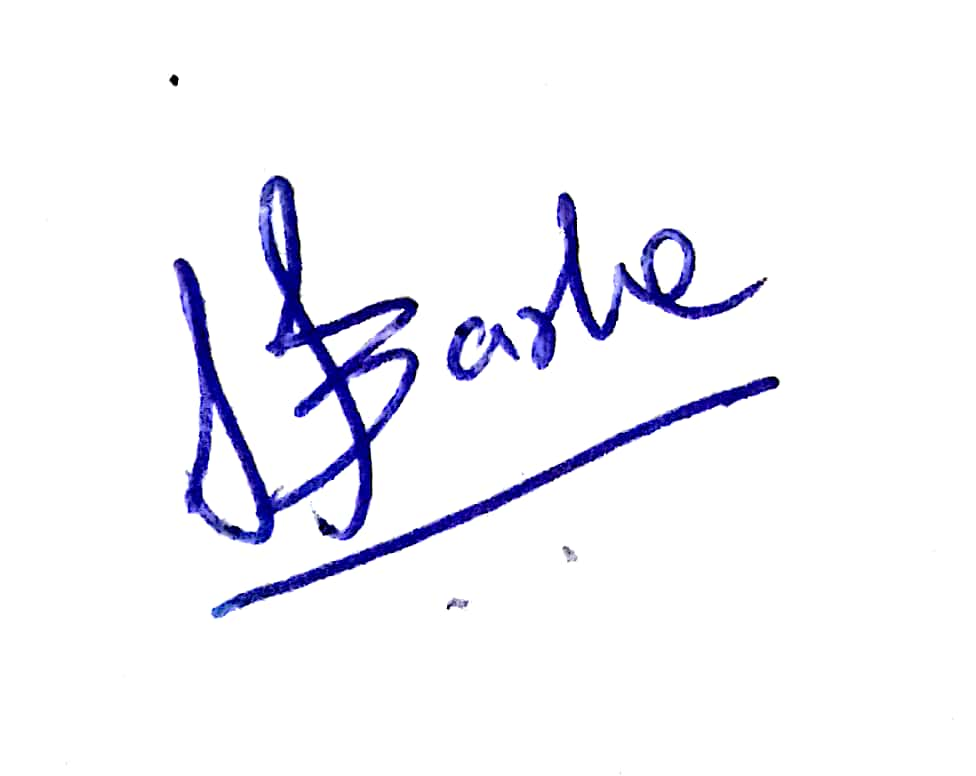
\includegraphics[scale=0.1]{images/sign.jpg}\\
   Mumbai, India                  &        Saiprasad Barke\\
  \rule{\textwidth/3}{0.4pt}      &   \rule{\textwidth/3}{0.4pt} \\
  
  Place, Date                     &   Signature
\end{tabular}

    \chapter*{Abstract}
\paragraph{}Understanding the key factors influencing the performance of depth estimation models is crucial in advancing computer vision applications such as 3D reconstruction, autonomous navigation, and augmented reality. This thesis explores these influencing factors within the context of the \framework {(\rmvd)}\cite{schroeppel2022benchmark} framework. We implement several models under the {\rmvd} umbrella, each uniquely different in architectural elements, to decipher their individual and collective impacts on depth estimation performance. We also examine the contributions of different data augmentation techniques and investigate the implications of the choice of training datasets. Further, we scrutinize the effects of manipulating data properties, like the number of source views, source selection approach, and diverse training hyperparameters, on the model's predictive performance and uncertainty estimation, offering insights into the principles that underlie the performance of {\mv} depth estimation models to empower future model design and refinement of depth estimation methodologies. \par
We observe that the depth estimation performance within the {\rmvd} framework is substantially influenced by the selection of the correlation layer and the feature extractor's capability to produce representative features. Additionally, the choice of input data and the way it's processed plays an indispensable role in model robustness. We also underscore the importance of normalizing features before correlation, a simple yet effective enhancement. The research also sheds light on potential avenues for future exploration, emphasizing the myriad of methodologies that, when aptly combined, can significantly boost the performance of {\mvs} models.
This report outlines the experimental setup, presents the results of the ablation study, and discusses potential directions for future research in the domain of depth estimation in a {\mv} setting. 
    \tableofcontents
    \listoffigures
    \listoftables
    \hypersetup{pageanchor=true}  % re-enable hyperlinking

    \pagestyle{fancy}
    \cfoot{\thepage}
    \renewcommand{\chaptermark}[1]{\markboth{#1}{#1}}
    \fancyhead[L]{{\textit{\scriptsize{Analysing Multi-view Depth Estimation in a common framework}}}}
    \fancyhead[R]{\textit{\footnotesize{\chaptername\ \thechapter\ --\ \leftmark}}}
    \renewcommand{\headrulewidth}{0.4pt}
    \renewcommand{\footrulewidth}{0.4pt}
    \mainmatter  % Arabic page numbers
    \chapter{Introduction}\label{chap:introduction}

\section{Background of the Problem}\label{sec:Background motivation of the problem}
    \paragraph{}Depth estimation is a cornerstone task in the realm of computer vision, with a wide array of applications, including 3D reconstruction, autonomous navigation, augmented reality, 3D printing, computational photography, computer video games, and preservation of cultural heritage. As we advance into an era defined by data and artificial intelligence, the importance of developing robust and efficient depth estimation models is paramount. When materials, viewpoints, and lighting conditions are well-defined, the task becomes more tractable. However, if any of these factors are not known, the problem typically becomes ill-posed. This is because a variety of combinations that involve geometry, materials, viewpoints, and lighting can result in identical photographs. In such cases, the ambiguity introduced by these unknown variables makes it difficult to uniquely determine the exact characteristics of the scene from the given images.\par 
    Humans possess an impressive capacity to solve such inverse problems, even when the solutions are uncertain. We can draw on our prior knowledge to make estimations about the size, arrangement, and coarse proximity of objects in the environment in relation to our own position and between the objects themselves. This proficiency can be attributed to previous experiential interactions with diverse objects and contexts, culminating in constructing cognitive priors that facilitate an insightful understanding of the visual attributes and spatial interconnections within the three-dimensional world around us. For decades, computer scientists have worked hard to recreate this amazing ability that we take for granted to enable computers to do the same. Inspired by the human binocular vision system, stereo matching and its extension {\mvs} (MVS)\cite{Seitz2006} based depth estimation models have garnered immense attention. In particular, {\mvs} models have become extremely successful due to their ability to take advantage of multiple views of a scene to produce accurate depth maps. \par
    While traditional {\mvs} methods have been successful to some extent, they often rely heavily on handcrafted features and similarity measures. This leads them to have limitations in handling poorly textured regions, and the models may struggle with occlusions or varying lighting conditions. With the rise of deep learning and especially Convolutional Neural Networks (CNN)\cite{lecun1997} and in recent years, the Visual Transformer(ViT)\cite{dosovitskiy2021image, ranftl2021vision, amir2021deep}, depth estimation has seen a paradigm shift, with models now capable of learning features directly from data and achieving superior performance. This, combined with the growing accessibility of extensive training datasets, has opened a new era of {\mvs} methodologies\cite{Seitz2006}. These approaches address the complex inverse problem of inferring depth information from RGB images.\par
    However, it has been observed in practice that the performance of these models depends on various factors, such as the underlying network architecture, training datasets, data augmentations, and several hyperparameters of the network and training setup. It has also been observed that models trained on a specific data modality do not generalize well to other modalities without significant adaptations and fine-tuning. This robustness characteristic is extremely important in the real world. In practical settings involving multi-camera layouts, we often have access to camera positions but lack depth range and alignment details of the ground truth and the predicted depth maps. Deep learning MVS methodologies aim to accurately determine relevant depth maps and their appropriate scales from this stream of visual data.\par 
    In this thesis, we explore which combinations of the factors mentioned above yield superior generalization results through different data modalities, particularly in challenging situations such as areas with intricate structures, sections without texture, reflective surfaces, zones with pronounced gradients, scenes involving minor camera movements, and instances of occlusions.


\section{A Brief Overview of \rmvd}\label{sec:A brief overview of \rmvd}
    \paragraph{}In this study, we take a closer look at the {\framework} framework\cite{schroeppel2022benchmark}, which provides a common ground to evaluate {\mv} depth models on their generalization capabilities in various domains. The framework has also given us the {\dispn} based {\rmvd} depth estimation model and a novel input image data augmentation technique called \textit{Scale Augmentation}\cite{schroeppel2022benchmark}. This approach has attracted much attention in the community by demonstrating robust cross-domain scale-agnostic {\mv} depth estimation.\par
    The framework also introduces the {\framework} benchmark \cite{schroeppel2022benchmark} founded on existing datasets with different modalities. This benchmark offers a three-fold evaluation protocol. Firstly, it gauges the performance of estimated depth maps across distinct data domains through a zero-shot assessment paradigm. Second, it quantifies uncertainties using the Area-Under-the-Sparsification-Error-Curve (AUSE)\cite{Ilg2018} metric. Additionally, the benchmark encompasses an absolute evaluation scenario motivated by practical use cases, where precise camera poses are provided to the model. The benchmark emphasizes depth estimation's generalization capabilities rather than just performance on specific datasets. It is proposed as an additional evaluation tool alongside traditional benchmarks such as KITTI, ScanNet, DTU, Tanks and Temples, and others. Overall, {\framework} offers a comprehensive platform to evaluate the generalization capabilities of depth estimation models in various domains, addressing both depth prediction and associated uncertainties.\par
    Despite the effectiveness of the {\rmvd} framework, the complexity and multifaceted nature of the {\mvs} raise several intriguing questions. How do individual components of the network architecture impact overall performance? What is the role of input data augmentations, and how do they affect the model's ability to generalize? How do the choice of data sets and the properties of the data influence performance? Also, how do the various hyperparameters of the models and the training setup steer the accuracy and efficiency of the models? \par

\section{Ablation Study and its Objectives}\label{sec:Ablation study and its objectives}
    \paragraph{}In this thesis, we aim to address these questions systematically. To this end, we conducted an extensive ablation study with the {\rmvd} framework, where we investigated the contribution of each of these components and factors to the overall performance of the model. We implemented different models within the {\rmvd} framework, each designed with different network architecture components. The API is written in a manner that makes it easier to conduct experiments in a plug-and-play fashion by making the interfaces of the different architectural components and the data loading for different datasets compatible. We then evaluate the impact of different input augmentations and assess the effect of training these models on various datasets in a known depth range setting. Furthermore, we consider a range of data properties, such as the number and sampling strategy of source views, and perform an in-depth exploration of the impacts of altering different hyperparameters in the network and training setup.\par
    Through our ablation study, we aim to shed light on the intricacies of depth estimation using {\mvs} and contribute to the understanding of the principles driving the performance of {\mv} depth estimation models. By identifying the most influential factors, we aim to inform the design of future models and enhance the effectiveness of depth estimation methodologies. 

\section{Report Structure}\label{sec:Report Structure}
    \paragraph{}The rest of this report is organized as follows: In \hyperref[chap:background]{Chapter 2}, we revisit the fundamental concepts of {\mv} geometry, disparity, and depth estimation in a {\mv} setting. We also have a detailed study of a typical {\mvs} depth estimation pipeline to explain the terminology used in this thesis. In \hyperref[chap:relatedwork]{Chapter 3}, we conduct a thorough literature review of existing research in the domain of depth estimation in an MVS setting. In \hyperref[chap:approach]{Chapter 4}, we present the details of our experimental setup, datasets, and model performance evaluation metrics. In \hyperref[chap:experiments]{Chapter 5} we discuss the results of our ablation study, organized by factors under consideration: \textbf{1)} \hyperref[sec:exp-arch]{network architecture components}, \textbf{2)} \hyperref[sec:exp-dataset-prop]{datasets, their properties and augmentations} and \textbf{3)} \hyperref[sec:exp-hyper]{hyperparameters of the training setup}. Finally, in \hyperref[chap:conclusion]{Chapter 6}, we draw conclusions from our findings and discuss potential avenues for future research in this domain. Model implementation details and quantitative analyses are presented in the \hyperref[chap:appendix]{Appendix}.



    \chapter{Background}\label{chap:background}
\begin{figure}[ht]
\centering
     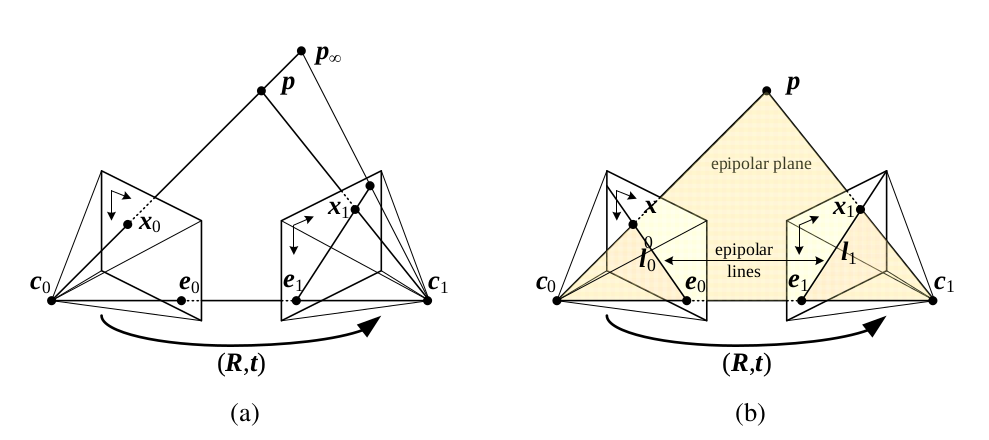
\includegraphics[width=1.0\textwidth]{images/epipolar.png}
      \caption[A typical Epipolar Geometry Setup]{\textbf{A typical Epipolar Geometry Setup.} $\mathbf{p}$ is the 3D point in the scene. $\mathbf{c_0}$ and $\mathbf{c_1}$ are the centers of the cameras. The triangle defined by the points $\mathbf{p,c_0,c_1}$ is the epipolar plane. The line $\mathbf{c_0}$,$\mathbf{c_1}$ that connects the two camera centers is the baseline, and the lines $\mathbf{x_0,e_0}$, and $\mathbf{x_1,e_1}$ are the epipolar lines. This image is obtained from \cite{Szeliski2010book}} 
       \label{fig:epipolar}
\end{figure}

In {\mvs} methodologies, camera matrices, source views, and reference views play crucial roles in establishing correspondences, predicting depth, and, ultimately, the reconstruction process.  There is an interesting relationship between the multiple cameras, the 3D point in the scene, and its projections in the image planes of the cameras. These relationships can be described by epipolar geometry.  \hyperref[fig:epipolar]{Figure 1} shows a standard epipolar geometry setup. This setup involves 2 cameras at $\mathbf{c_0}$ and $\mathbf{c_1}$ observing the same 3D point $\mathbf{p}$ in the scene. $\mathbf{x_0}$ and $\mathbf{x_1}$ are the projections of $\mathbf{p}$ on the image planes of the two cameras.\par 
First, we will define the terminology associated with epipolar geometry and the estimation of the depth/disparity. Then, in the subsequent sections, we will formalize the definitions and draw connections between the different concepts. 

\section{Relevant Terminology}

\begin{itemize}
\item \textbf{Epipolar Plane:} Epipolar plane is the plane defined by the centers of the cameras and a 3D point in the scene. In Figure \hyperref[fig:epipolar]{1}, the triangle defined by the points $\mathbf{p,c_0,c_1}$ is the epipolar plane. 
\item \textbf{Epipolar Line:} The intersections of the epipolar plane with the image planes are known as the epipolar lines. In Figure \hyperref[fig:epipolar]{1}, the two lines $\mathbf{x_0,e_0}$ and $\mathbf{x_1,e_1}$ are the epipolar lines.
\item \textbf{Epipoles:} The points of intersection of the baseline $\mathbf{c_0},\mathbf{c_1}$ with the image planes are the epipoles. In Figure \hyperref[fig:epipolar]{1}, the points $\mathbf{e_0}$ and $\mathbf{e_1}$ are the epipoles. 
\item \textbf{Epipolar Constraint:} It is the fundamental rule of epipolar geometry that states that any projection $\mathbf{x_0}$ of the 3D point $\mathbf{p}$ in one image must lie on the corresponding epipolar line $\mathbf{x_1, e_1}$ in the other image. This restriction greatly reduces the search space when attempting to match points between two images, from a 2D search to a 1D search along the epipolar line.
\item \textbf{Camera Matrices:}
A camera matrix represents the intrinsic (lens) and extrinsic (pose) parameters of a camera. It consists of a $3\times3$ matrix containing the intrinsic parameters such as focal length, principal point, and lens distortion coefficients, along with a $4\times4$ matrix representing the extrinsic parameters, which describe the camera's position and orientation in 3D space. Camera matrices are used to project 3D points onto the image plane and project 2D points back onto the 3D space when reconstructing the scene. 
\item \textbf{Homography:} A transformation $H$ that maps the points in one image plane to the corresponding points in another image plane.
\item \textbf{Homography Matrix:} An arbitrary $3\times3$ transformation matrix in a homogeneous coordinate space that represents the homography transformation.
\item \textbf{Homography Warping:} The process of applying a homography transformation to an image or part of an image so that the first image aligns with the second image. 
\item \textbf{Rectification:} The process of transforming stereo images so that their corresponding epipolar lines become collinear and parallel to the $x$-axis. This simplifies the search for the corresponding points from a 2D search to a 1D search. This leads to the two image planes being parallel to each other. 
\item \textbf{Rectified Images:} The images obtained after rectifying. The epipolar lines in these images are parallel to the $x$-axis.
\item \textbf{Image Correspondences:} This refers to the process or result of finding common features or points between two or more images. 
\item \textbf{Disparity:} The difference in the position of a 3D point observed in two different images. In rectified images, the disparity corresponds to the horizontal difference.
\item \textbf{Disparity Map:} An image in which the value of each pixel represents the disparity of that pixel between two stereo-rectified images.
\item \textbf{Depth Map:} An image in which the value of each pixel represents the estimated depth of that pixel in the scene.
\item \textbf{Source Views:}
In MVS, source views refer to a set of input images captured from different viewpoints around a scene. These views are used to extract visual information and establish correspondences between image points. Source views provide multiple perspectives that are necessary to accurately estimate the depth values in the scene. 
\item \textbf{Reference View:}
A reference view is a specific source view selected as a reference frame for the depth estimation process. It serves as an anchor image for calculating the depth map or point cloud of the scene. The other source views are then aligned and matched with the reference view to establish correspondences using the camera's intrinsic and extrinsics matrices to compute the depth information.
\item \textbf{View Selection Strategy:}
Choosing the right images as source and reference views is a crucial step in MVS. Each view has its own extrinsic camera parameters. These choices can significantly impact the accuracy and quality of the final reconstruction. A good strategy is to choose source views that cover the entire scene with adequate overlap and reference views that are centrally located or provide the most informative view of the scene with minimum occlusions and good illumination. 
\end{itemize}

\section{Epipolar Geometry and Image Correspondences}\label{sec:3dgeom}
Now that we have established a foundation of 3D geometry vocabulary, we will thoroughly analyze the formal definitions of the abovementioned concepts. Given a pixel in one image, how can we compute its correspondence in another image efficiently and reliably? For the scenarios discussed in this thesis, we have the positions and calibration data of the cameras available.\par
In  \hyperref[fig:epipolar]{Figure 1a}, we can see how one pixel $\mathbf{x_0}$ projects to an epipolar line segment in the other image. One end of the segment is defined by the projection of the original viewing ray at infinity, denoted as $\mathbf{p\infty}$. The other end is defined by the projection of the original camera center, $\mathbf{c_0}$, into the second camera, known as the epipole $\mathbf{e_1}$. By projecting the epipolar line from the second image back into the first, we can create another line bounded by the corresponding epipole $\mathbf{e_0}$. These line segments can be extended to infinity, creating a pair of corresponding epipolar lines as shown in  \hyperref[fig:epipolar]{Figure 1b} that are the intersections of the two image planes and the epipolar plane that is bounded by both camera centers $\mathbf{c_0}$ and $\mathbf{c_1}$ and the 3D point of interest, $\mathbf{p}$ \cite{Hartley2004}. Now, let us examine the different coordinate systems and camera matrices.\par
The commonly used coordinate systems in Computer Vision are:
\begin{enumerate}
    \item \textbf{World coordinate system (3D):} This is a 3D cartesian coordinate system with an arbitrary origin. It is the base reference system. A point in this coordinate system can be denoted as $\mathbf{P_w} = (X_w, Y_w, Z_w)$.
    \item \textbf{Camera coordinate system (3D):}  This is also a 3D cartesian coordinate system with its origin at the origin of the camera. The coordinates are measured with respect to the camera center and orientation. A point in the camera coordinate system is denoted as $\mathbf{P_c} = (X_c, Y_c, Z_c)$. One can go from the world coordinate system to the camera coordinate system using the camera extrinsics matrix. This $4\times4$ matrix can be broken down into a rotational $\mathbf{R}_{3\times3}$ and a translational $\mathbf{t}_{3\times1}$ component. The camera coordinates can be obtained from the world coordinates using the extrinsics matrix by \hyperref[eq:world-to-camera]{Equation1}.
    \begin{equation}
        \begin{pmatrix}
            \mathbf{P_c}^\intercal \\
            1
        \end{pmatrix}_{4\times1}
        = 
        \begin{bmatrix}
            \mathbf{R}_{3\times3} & \mathbf{t}_{3\times1}\\
            \mathbf{0}_{1\times3} & \mathbf{1}_{1\times1}
        \end{bmatrix}_{4\times4}
        \begin{pmatrix}
            \mathbf{P_w}^\intercal \\
            1
        \end{pmatrix}_{4\times1}
    \end{equation}\label{eq:world-to-camera}
\item \textbf{Image coordinate system (2D):} This coordinate system is obtained when the 3D camera coordinates are projected onto the 2D image plane. This projection operation results in the loss of depth information or the Z coordinate. A point in the image coordinate system is denoted as $\mathbf{P_i} = (X_i, Y_i)$. For the pinhole camera model, the 2D image plane is located at focal length $f$ away from the camera. This projection involves the camera intrinsics matrix. The camera intrinsics matrix is given by \hyperref[eq:cam-intrinsic]{Equation 2}.
\begin{equation}
    \mathbf{K}
    =
    \begin{bmatrix}
        f_x & s & c_x \\
        0 & f_y & c_y \\
        0 & 0 & 1
    \end{bmatrix}
\end{equation}\label{eq:cam-intrinsic}
Here, assuming square pixels, $f_x$ = $f_y$ = $f$ is the focal length of the camera. The skew factor is denoted by $s$, which is usually $0$. $c_x$ and $c_y$ denote the coordinates of the camera's center.
We can obtain the 2D image coordinates from the 3D camera coordinates with \hyperref[eq:image-from-cam]{Equation 3}:
\begin{equation}
    \mathbf{X}_i = f\frac{\mathbf{X_c}}{\mathbf{Z_c}}\hspace{1cm} \text{and} \hspace{1cm}\mathbf{Y}_i = f\frac{\mathbf{Y_c}}{\mathbf{Z_c}}
\end{equation}\label{eq:image-from-cam}
This can also be represented in matrix form by \hyperref[eq:image-from-cam-matrix]{Equation 4}:
\begin{equation}
    \begin{pmatrix}
            \mathbf{P_i}^\intercal \\
            Z_c
        \end{pmatrix}
        = 
        \begin{bmatrix}
            f & 0 & 0 &0\\
            0 & f & 0 &0\\
            0 & 0 & 1 &0
        \end{bmatrix}
        \begin{pmatrix}
            \mathbf{P_c}^\intercal \\
            1
        \end{pmatrix}
\end{equation}\label{eq:image-from-cam-matrix}
\item \textbf{Pixel coordinate system (2D):} Pixel coordinate system is obtained when the image coordinate system is discretized. Another pair of parameters called the pixel width $\rho_u$ and the pixel height $\rho_v$ come into play for this transformation. The pixel coordinates can be calculated by dividing the image coordinates by the width and height of the pixels. Since the pixel coordinate system begins at the top-left of the image, we also require the remaining two parameters of the camera intrinsics matrix, $c_x$ and $c_y$. This is given in \hyperref[eq:pix-from-img]{Equation 5}.
\begin{equation}
    \mathbf{X}_i = \frac{f}{\rho_u}\frac{\mathbf{X_c}}{\mathbf{Z_c}} + c_x\hspace{1cm} \text{and} \hspace{1cm}\mathbf{Y}_i = \frac{f}{\rho_v}\frac{\mathbf{Y_c}}{\mathbf{Z_c}} + c_y
\end{equation}\label{eq:pix-from-img}
This can be represented in matrix form by \hyperref[eq:pix-from-img-matrix]{Equation 6}.
\begin{equation}
    \begin{pmatrix}
            u\\
            v\\
            w
        \end{pmatrix}
        = 
        \begin{bmatrix}
            \frac{1}{\rho_u} & 0 & c_x \\
            0 & \frac{1}{\rho_v} & c_y \\
            0 & 0 & 1 
        \end{bmatrix}
        \begin{pmatrix}
            \mathbf{X_i}^\intercal \\
            \mathbf{Z_c}
        \end{pmatrix}
\end{equation}\label{eq:pix-from-img-matrix}
Using the above equations, we get \hyperref[eq:world-to-pix]{Equation 7}, which is the transform from world coordinates to pixel coordinates using the camera intrinsics and extrinsics matrices. This product of the intrinsics and the extrinsics matrices is known as the projection matrix $\mathbf{P}$:
\begin{equation}
    \begin{pmatrix}
        u\\
        v\\
        w
    \end{pmatrix}
=   \underbrace{\begin{bmatrix}
        \frac{f}{\rho_u} & 0 & c_x &0 \\
        0 & \frac{f}{\rho_v} & c_y &0\\
        0 & 0 & 1 &0
    \end{bmatrix}}_\text{Intrinsics} 
            \underbrace{\begin{bmatrix}
            \mathbf{R}_{3\times3} & \mathbf{t}_{3\times1}\\
            \mathbf{0}_{1\times3} & \mathbf{1}_{1\times1}
        \end{bmatrix}_{4\times4}}_\text{Extrinsics}
        \begin{pmatrix}
            \mathbf{P_w}^\intercal \\
            1
        \end{pmatrix}_{4\times1} 
        \text{and} \hspace{5mm}\mathbf{P}=\mathbf{K[R|t]}
\end{equation}\label{eq:world-to-pix}
\end{enumerate}


In the stereo configuration depicted in \hyperref[fig:epipolar]{Figure 1}, several foundational assumptions are essential. Both cameras exist within a canonical configuration. The term "canonical" in stereo vision refers to a rectified scenario wherein the epipolar lines of the two cameras are horizontally aligned. Such rectification considerably streamlines the process of disparity estimation. Further reinforcing this simplification, both cameras are assumed to possess identical intrinsic matrices, denoted by $\mathbf{K}$. In this setup, we also assume that the origin of the world coordinate system is at the first camera, with the second camera offset first by a rotation $\mathbf{R}$ and then by a translation $\mathbf{t}$. Specifically, in this harmonized environment, determining disparity for a given plane at depth $d$ equates to computing the corresponding homography, which is a projective transformation for that specific depth. Since the image planes in a rectified setup are parallel, the transformation induced by a plane-specific homography invariably results in a spatial shift. Every point on the delineated plane undergoes this shift, which is equivalent in magnitude to the plane's established disparity.

This foundational stereo model resembles the paradigm found in Multi-View Stereo (MVS). Within the MVS framework, source image projections are methodically warped onto fronto-parallel planes. These planes reside within the frustum of a specified reference camera and span diverse depth levels. As these planes undergo spatial adjustments, either approaching or receding from the camera setup, the inherent disparity alters. This change in disparity underscores the principle that every depth-defined plane possesses a unique disparity value and, by extension, a distinctive homography.

Next, we will discuss the connection between disparity and depth, as well as introduce cost volumes and various types of loss functions in the following section.

\section{Disparity and Depth}\label{sec:depthestim}

As a problem domain, depth estimation aims to predict the distance from the camera to each pixel in an image or a sequence of images. In the context of MVS, where the camera parameters are known, the problems of depth or disparity estimation and that of solving for the 3D geometry of the scene are the same, and these are, in turn, equivalent to solving the problem of accurately determining the point correspondences across the images \cite{Furukawa2015}. Knowing the likelihood and uncertainty of estimating these point correspondences is also important. \par
There is a straightforward inverse relationship between depth $Z$ and disparity $d$ for rectified images. This is given by \hyperref[eq:depth-disp]{Equation 8}. \cite{Szeliski2010book, Okutomi1993}
\begin{equation}
    d = f\frac{B}{Z}
\end{equation}\label{eq:depth-disp}
where $f$ is the focal length in pixels, and B is the baseline length connecting the two camera centers. In such a case, extracting depth from a set of images is equivalent to estimating the disparity map $d(x, y)$ \cite{Szeliski2010book}.\par
Simply put, objects closer to the cameras have larger disparities than those farther away. By computing the disparity for every pixel or feature point between two stereo images, a disparity map can be generated. This can then be converted into a depth map using the camera's parameters and geometry. This interchangeability of depth and disparity also holds for the {\mvs} setup. However, it is worth noting that MVS does not typically employ rectified images. Instead, it involves multiple scene images captured from varied viewpoints that might have substantial angular differences. This is where cost volumes come into play. In {\mvs}, the cost volume is a 3D volume computed as the similarity between the warped source features and the reference image feature at multiple fronto-parallel planes of the reference camera frustum. One of the benefits of using cost volumes is that they do not require rectified images, making them a more viable option than obtaining correspondences between a pair of images in a general 3D setup. \par

The goal of learning-based {\mvs} depth estimation is to learn a predictor $f_\theta$ that can predict a depth map $\hat{D}$ that is a close approximation of the ground truth depth map $D$. This can be written as a minimization of \hyperref[eq:depth-loss]{Equation 9} \cite{Laga_2022}:
\begin{equation}
    L(\mathbf{I}) = d(f_{\theta}(\mathbf{I}), D) 
\end{equation}\label{eq:depth-loss}
Here, $d(\cdot,\cdot)$ is any similarity metric such as $L1$, $L2$ or a classification loss between the predicted depth map $f_{\theta}(\mathbf{I})$ and the ground truth $D$. ${\theta}$ is the set of model parameters. \par
Given the continuous nature of depth values, this task is generally approached in the context of deep learning as a regression problem \cite{Yao2018, cheng2020deep, Gu2020, Yang2020}. Regression involves using a soft-argmin operation to generate a depth map from the 3D cost volume, with each depth hypothesis being weighted differently. This method allows for sub-pixel depth estimation by summing discrete weighted depth hypotheses. However, it can result in various combinations of weights producing the same depth, making it harder for the model to converge and increasing the risk of overfitting the training data, thereby reducing the generalizability of the model.\par
This task is also approached as a classification problem by some methodologies \cite{Zhang2020, Yao2019}. Such an approach predicts the likelihood of each depth hypothesis in the 3D cost volume, selecting the depth map corresponding to the maximum probability. The main advantage of a classification method is that it constrains the cost volume via the cross-entropy loss, which makes it more robust than regression methods. Still, there is no exact depth due to discretization.\par
In the following section, we will look at depth estimation in a {\mvs} setup where the epipolar constraint does not hold. 


\section{Depth Estimation with Multi-view Stereo}\label{sec:multiviewster}

Furukawa {\etal} \cite{Furukawa2015} defined the depth prediction problem as a 1D feature matching problem along the epipolar lines. {\mvs} (MVS) is a class of computer vision methods that aim to reconstruct a 3D model of a scene from multiple images taken from different viewpoints \cite{Seitz2006}. These techniques take advantage of the parallax effect, which is the apparent displacement of an object caused by a change in the observer's point of view. The greater the distance between the viewpoints, i.e., the length of the baseline, the more pronounced the parallax effect.

Depth estimation in the context of MVS involves determining the distance of each pixel (or a group of pixels) from the camera to construct a depth map, which can generate a 3D scene model. This process involves finding correspondences between different images and using epipolar geometric constraints to triangulate the position of each point. For the sake of simplicity of explanation, we use the words "images" and "features" interchangeably. However, it should be noted that state-of-the-art {\mvs} methodologies employ features extracted from images to find correspondences and matching costs. 

Okutomi et al. in \cite{Okutomi1993} discretized the depth space and turned the task of binocular stereo depth estimation into a classification problem. The plane sweep algorithm \cite{Collins1996ASA} applies the same discretization principle to a {\mvs} setup. We have already established in the previous sections the relationship between finding matching correspondences between images, depth/disparity estimation, and the 3D geometry of the scene. The zero-mean normalized cross-correlation (NCC) is one of the most common and successful similarity measures used in {\mvs} algorithms. Before computing this similarity metric, the source image is warped to the reference camera frustum and projected across different depth levels in this frustum. This is achieved by using homography warping with the planesweep algorithm. In this section, we will dive into the planesweep algorithm and the cost volumes of the feature matching costs that form the core of the MVS methodologies studied in this thesis. 

Collins stated, "For a multi-image technique to be considered truly effective, it should be able to handle any number of images, have an algorithmic complexity of $O(n)$ in terms of the number of images used $(n)$ and should utilize all the images in an equal manner." \cite{Collins1996ASA}. \hyperref[fig:psw]{Figure 2} shows the plane sweep operation. This method operates under the assumption that the regions in space where multiple viewing rays of image features converge are highly probable to be the 3D positions of observed features within the scene. After the source image has been projected to the reference image frustum at multiple depth hypotheses and a particular point in space at depth $z$, captured by different cameras, appears similar, then that point is likely a real 3D point at depth $z$ from the camera.\par
\begin{figure}[h]
\centering
     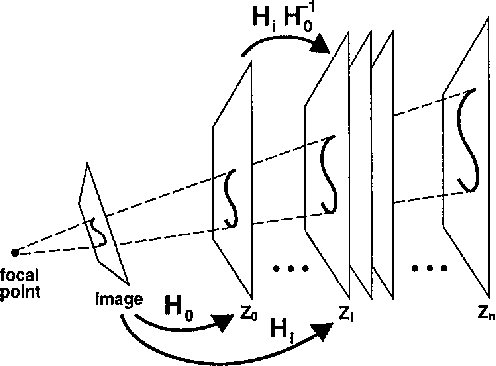
\includegraphics[width=0.5\textwidth]{images/psw.png}
      \caption[Plane sweep operation]{\textbf{Plane sweep operation.} Pixels from each image are back-projected onto successive positions $Z = z_i$ of a plane that sweeps through the camera's frustum with homography $H_i$. $H_0$ is the homography that maps the image points to the plane at $Z = z_0$. By combining the two, we can say that the homography that maps pixels between the planes $Z = z_0$ and $Z = z_i$ directly, by forward projection from the $z_0$ plane onto the image, then back-projection to the $z_i$ plane, can be written as $H_i\inv{H_0}$. This image is taken from \cite{Collins1996ASA}}.
       \label{fig:psw}
\end{figure}
The entire depth range in the reference frustum is discretized. This is a common step in many MVS algorithms and is essential for constructing the cost volume. The depth $d_i$ at the $i^{th}$ plane can be calculated as:
\begin{equation}
    d_i = \mathbf{D_{min}} + i \times \frac{\mathbf{D_{max}-D_{min}}}{N-1} \hspace{0.5cm} \text{for} \hspace{0.5cm} i=0, \dots, N-1
\end{equation}\label{eq:dist-discrete}
Here, $[\mathbf{D_{min}}, \mathbf{D_{max}}]$ is the depth range of the scene. $N$ is the number of depth planes in the cost volume. In the camera's frustum, each of these depth levels corresponds to a "plane" parallel to the image plane of the camera. Then, every pixel in the reference image will have $N$ depth hypotheses corresponding to these $N$ planes. The task of the MVS algorithm will be to determine the most likely depth value for each pixel. Increasing $N$ reduces the discretization errors in the results and increases the number of parameters in the network and, thus, the GPU memory. In this thesis, we use $N=256$ for {\rmvd} and $N=128$ for {\mvsn}.

Once the depth has been discretized, we must align the pixels between the reference and the source images using a homography $\mathbf{x'} ~ \mathbf{H_k}(d_i)\cdot \mathbf{x}$ where $∼$ indicates equality up to scale \cite{Szeliski2010book, Yao2018}.  Only then can we measure the similarity between the reference and the source features. In the depth hypothesis $d_i$, we first project all pixels of a source feature into space with $d_i$ and then back-project these points through the reference camera. Thus using \hyperref[eq:world-to-pix]{Equation 7} and the projection equation from \hyperref[fig:psw]{Figure 2}, the homography between the $k^{th}$ source image and the reference image at depth $d_i$ can be obtained as:
\begin{equation}
    \mathbf{H_k}(d_i)= d_i\mathbf{K_0T_0\inv{T_k}\inv{K_k}}
\end{equation}\label{eq:homography}
where $\mathbf{K_0}$ and $\mathbf{T_0}$ are the camera intrinsics and extrinsics matrices of the reference image. \cite{zhu2021deep}

After the depth discretization and the warping operation, we can now construct a cost volume. This is essentially a 3D volume where one dimension corresponds to the image's width, another to its height, and the third to the depth levels.
Each voxel 3D pixel in this volume corresponds to a pixel in the reference image and a specific depth level. The voxel's value or "cost" represents how well that depth matches the observations from the other images based on some metric. Depth estimation involves finding the depth level with the minimum cost for each pixel and producing a dense depth or disparity map. The methods explored in this thesis use normalized cross-correlation as a similarity metric. \par
One of the baselines {\mvsn} does not employ any correlation but only warps the source features to the reference features and fuses the cost volumes with a variance-based strategy. {\rmvd} uses the Dispnet correlation layer \cite{Mayer2016} that employs the full correlation and decimates the feature dimension. Schröppel \etal in the {\rmvd} framework \cite{schroeppel2022benchmark} improved the plane sweep homography warping described above for the pairwise cost volume construction. This is done by explicitly enforcing the epipolar constraint on the sampling points in the source image before the warping and correlation operations. The sampling points for a point on the reference image are constrained to its epipolar line in the source image at the different depth levels. This reduces the search space for matching points to a 1D search along the epipolar line. As a result of this explicit constraining, the correlation costs are computed between a more accurately warped source and reference image. \hyperref[fig:cvc]{Figure 3} shows the cost volume construction operation in a typical MVS setup. All the models implemented in this thesis use this improved version of the planesweep warping operation. \par
In the next section, we take a look at the complete MVS pipeline and describe in detail each component of the pipeline. 


\section{Multi-view Depth Estimation Pipeline}\label{sec:mvspipeline}
When using deep learning for depth estimation in an MVS setting, the network is typically trained to learn these complex mappings from the input images to the feature maps, cost volumes, and a corresponding depth map guided by a suitable loss function. A common approach involves feeding the network with pairs of images and their corresponding disparity (or depth) maps during the training phase. The network learns to extract features from the images and associate the similarity between the images with the depths. This learned model can be used to predict depth maps from new pairs of images.

One significant advantage of using deep learning for this task is that networks can learn to handle a wide range of complex scenes and lighting conditions, which can be challenging for traditional MVS methods. Moreover, using convolutional layers in these networks allows them to consider the local context in the images, which can significantly improve the accuracy of depth estimation.

An example of a deep learning method for MVS is the MVSNet framework, which uses a differentiable homography warping \cite{Yao2018} layer to aggregate information from multiple views into a cost volume using a variance-based fusion and a 3D CNN to regress the depth map from this cost volume. This framework allows for end-to-end training and can handle an arbitrary number of input views. 

The standard multiview depth estimation pipeline consists of several stages that collectively generate accurate depth maps or point clouds from multiple input images. The main components of this pipeline include a feature encoder, a matching costs computation and aggregation unit, and a component to denoise the aggregated costs known as the regularization unit. The final depth is estimated from the denoised costs. We will dive into each of these components, their different flavors, and the network architectures that use these components as their basis. 

\begin{enumerate}
\item \textbf{Input and Preprocessing:} The input to the pipeline is a set of images of a scene taken from different viewpoints (source views), with one image selected as the reference view. Input images are often preprocessed, including normalization and resizing, to ensure that they are in a suitable format for a neural network. To maintain the integrity of our experiments, we have fixed the input sizes and the sizes of the evaluation data. If a model is trained with smaller inputs due to memory constraints on the GPU, it is explicitly stated. All sizes are multiples of 32. This addresses the size mismatch in spatial dimensions caused by strided convolutional operations on input tensors and skip connections to a layer.

\item \textbf{Feature Extraction:} In this stage, a Convolutional Neural Network (CNN) is used to extract feature maps from input images. The feature extractor scans the images and learns to identify patterns and structures that are important for depth estimation, such as edges, corners, and textures. This process reduces the high-dimensional image data to a more manageable, lower-dimensional form that still contains the information necessary for depth estimation. In this thesis, we examine the feature encoders of MVSNet and DispNet. We also explore the effects of using a multiscale architecture such as a UNet \cite{ronneberger2015unet}  for feature extraction and also look at fusing the learned features with features generated by a pre-trained ViT such as DINO \cite{caron2021emerging}. 

\item \textbf{Cost Volume Construction:} To find correspondences between different views, a cost volume is often constructed. The cost volume effectively represents the likelihood that each pixel in the reference image has a certain depth. We described the construction of a pairwise cost volume using different correlation types and homography warping with the plane sweep algorithm in detail in \hyperref[sec:multiviewster]{Section 2.4} and \hyperref[sec:depthestim]{Section 2.3}. The individual pairwise cost volumes of the reference and source features are fused using different strategies to obtain the aggregated cost volume. The learned fusion involves learning weights for each pairwise cost volume using a 2D or 3D CNN. Views with more occluded points are given less weight in the aggregated cost volume. Average fusion simply fuses all pairwise volumes equally. Variance-based fusion, which is used in {\mvsn} \cite{Yao2018}, compares the variance of the warped source features and the reference feature to fuse the warped volumes. In this thesis, we examine all three fusion strategies. 
\begin{figure}[ht]
\centering
     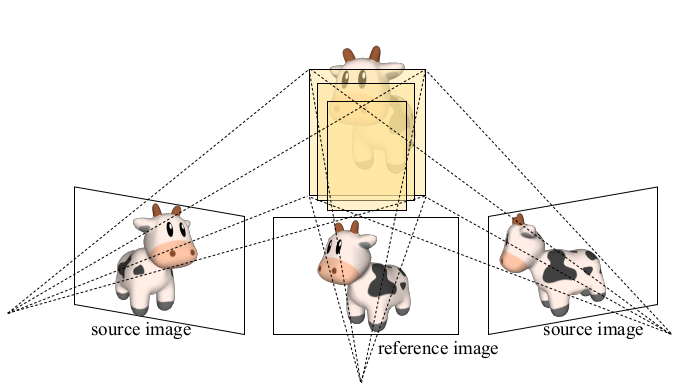
\includegraphics[width=0.75\textwidth]{images/cvc.png}
      \caption[Cost volume construction]{\textbf{Cost volume construction.} Using homography warping with a planesweep volume along the reference camera frustum and computing the matching costs at the different depth planes. This image is taken from \cite{zhu2021deep}.} 
       \label{fig:cvc}
\end{figure}
\item \textbf{Cost Volume Processing and Depth Map Estimation:} The cost volume is typically processed using a 3D CNN \cite{Yao2018, Zhang2020, Gu2020, Yang2020}, or RNN \cite{Yao2019} that aggregates and regularizes information across different views and depths to robustly estimate the depth map of the reference view. This is an essential step due to cost volumes being inherently noisy due to occlusions, poor texture and lighting, and non-Lambertian surfaces. Some techniques use a coarse-to-fine pattern to better estimate the depth and reduce memory consumption. The first level of the network predicts a coarse depth map. This is used as input for subsequent levels to yield finer results. Multiscale feature extractors are used to obtain features at different resolutions. The low-resolution features are used at the coarse level, and the high-resolution features are used as input to the finer levels along with the coarse depth map from the previous level. There are also different implementations of this strategy. Some methods simply use cascade fusion, such as CasMVSNet and CVP-MVSNet\cite{Gu2020, Yang2020} while others, such as Vis-MVSNet \cite{Zhang2020}, also use the uncertainty map to weigh depth residuals. In this thesis, we explore regularization using a regular 2D UNet for {\rmvd} and 3D UNet for {\mvsn}. We also look at cascade warping and implement and experiment with a coarse-to-fine pattern for both these baselines. The coarse-to-fine architecture is shown in \hyperref[fig:ctf]{Figure 4}

\begin{figure}[ht]
\centering
     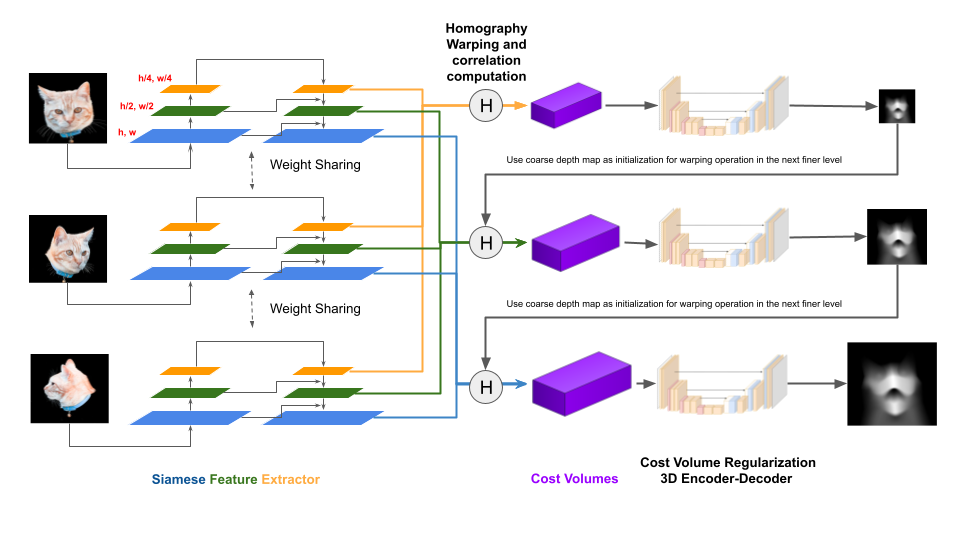
\includegraphics[width=1\textwidth]{images/coarse-to-fine.png}
      \caption[Coarse-to-fine pattern]{\textbf{Coarse-to-fine pattern.} This figure shows a typical coarse-to-fine design. Cost volumes at finer levels are constructed using the coarser depth predictions as initialization. In this figure, a single 3D UNet is used as the regularization network. 3D UNets in a stacked hourglass configuration~\cite{newell2016stacked} are also used to regularize raw cost volumes (in purple). The cost volumes at finer levels have a smaller depth range centered around the previous coarse depth predictions and are coupled with an adaptive subdivision of depth intervals for finer levels. Multilevel features with different spatial resolutions and channel depth are used to construct the cost volumes and depth maps at different levels. A multilevel feature extractor, such as a feature pyramid network or a 2D UNet, can be used for this purpose.}
\label{fig:ctf}
\end{figure}

\item \textbf{Refinement:} The initial depth map from the previous stage is often coarse and may contain inaccuracies. Therefore, it is common to refine the depth map using various methods. This could involve an additional CNN that takes the initial depth map and the reference image as input and learns to predict corrections to the depth values. The network can be trained to minimize the difference between its predictions and ground truth depth maps, if available. In this thesis, we only look at the fundamental elements of the MVS pipeline discussed previously and their interaction. We do not look at the effects of additional image-refinement strategies. 

\item \textbf{Training:} The entire pipeline can be trained from beginning to end using supervised learning, as ground-truth depth maps are available. If not, unsupervised or self-supervised methods can be used, where the training signal comes from photometric consistency or other cues. All experiments in this thesis are performed in a supervised manner, with the correlation between the source and reference images as a signal to guide the entire process. 

\item \textbf{Testing and Evaluation:} Once the pipeline is trained, it can be used to estimate depth maps from new multiview image sets. The datasets used to evaluate and train networks are discussed in detail in \hyperref[sec:datasets]{Section 4.2}. The quality of the depth maps can be evaluated using various metrics, such as mean absolute error or mean squared error, if ground truth is available. The metrics are discussed in \hyperref[sec:metrics]{Section 4.3}. Visual inspection and downstream tasks can also be used for evaluation.

\end{enumerate}\par
There are several versions of this pipeline that are tailored to different tasks, data availability, and current research advancements. Some of the recent approaches suggest the inclusion of transformer architectures, attention mechanisms, and other advanced techniques such as coarse-to-fine architecture, feature pyramids, and pre-trained vision transformers as feature extractors in the pipeline to enhance the accuracy of depth estimation. In the following chapter, we will conduct a comprehensive evaluation of these methodologies.




    \chapter{Related Work}\label{chap:relatedwork}

\paragraph{} This chapter contains a comprehensive overview of the literature on the application of deep learning-driven {\mvs} methods to the problem of Depth Estimation. A typical setup to tackle this problem involves taking multiple perspectives of a scene from different viewpoints. These images are then used as input to compute a depth map of the scene. Traditionally, the depth estimation process with {\mvs} is decomposed into three important steps: extraction of features from input images, aggregation of matching costs from features, and prediction of depth from aggregated costs. We divide our literature review into sections as per these three steps. \par 
In Section \hyperref[sec:relwork-featex]{2.1}, we examine the relevant literature for feature extraction. In Section \hyperref[sec:relwork-dispes]{2.2}, we explore the state of the art in the domain of disparity estimation and cost volume construction, which is a fundamental task for any stereo methodology. Finally, in Section \hyperref[sec:relwork-mvs]{2.3}, we present the state of the art in the domain of deep learning-driven {\mvs} methods for depth estimation. For the purpose of this review, we use the terms "disparity" and "depth" interchangeably. Depth is easily obtained as it is inversely proportional to disparity. Both depth and disparity estimation employ similar methodologies.

%%%%%%%%%%%%%%%%%%%%%%%%%%%%%%%%%%%%%%%%%%%%%%%%%%%%%%%%%%%%%%%%%%%%%%%%%%%%%%%%%%%%%%%%%%%%%%%%%%%%%%%%%%
\section{Feature Extraction}\label{sec:relwork-featex}
This is a crucial step in enhancing the fidelity of depth estimation and ensuring the robustness of the correspondences for computing the matching costs between views. Feature descriptors ensure better correspondences compared to RGB color images, particularly in regions that lack definitive texture or have repetitive patterns, and also support photometric and geometric consistency across the different views.\par
Classical methodologies such as Scale-Invariant Feature Transform (SIFT) \cite{lowe1999object}, Speeded-Up Robust Features (SURF) \cite{10.1007/11744023_32}, Oriented FAST and Rotated BRIEF (ORB) \cite{rublee2011} and neural network architectures involving convolutional neural networks (CNN) such as UNets \cite{ronneberger2015unet}, VGGs \cite{simonyan2015deep}, ResNets \cite{he2015deep} are employed to discern and characterize salient regions within images. Zbontar and LeCun \cite{Zbontar2016} introduce a deep Siamese network to compute matching costs. Feature pyramid networks (FPN) \cite{lin2017feature} are popular feature extractors that produce multiscale features that are used for downstream MVS tasks. Chang {\etal} in PSMNet \cite{chang2018pyramid} propose a pyramid stereo matching network to take advantage of global context information using spatial pyramid pooling (SPP) \cite{He_2014} and dilated convolutions \cite{yu2016multiscale} to expand receptive fields. Recently, the use of Visual Transformers (ViT) \cite{dosovitskiy2021image, cao2022mvsformer, ranftl2021vision, amir2021deep} for feature extraction gives superior results compared to the use of only FPNs or UNet. In this thesis, we implement the FPN and UNet feature extractors. We also use a pretrained DINO ViT to augment the learned features. 
%%%%%%%%%%%%%%%%%%%%%%%%%%%%%%%%%%%%%%%%%%%%%%%%%%%%%%%%%%%%%%%%%%%%%%%%%%%%%%%%%%%%%%%%%%%%%%%%%%%%%%%%%%
\section{Cost Volumes and Disparity Estimation}\label{sec:relwork-dispes}
Disparity estimation is most commonly associated with stereo vision, where two cameras capture images of the same scene from slightly different viewpoints. Disparity represents the horizontal difference in the $x$ coordinates of congruent pixels in rectified images. Image rectification simplifies the problem of calculating the 3D point coordinates in the scene to a 1D search on the same epipolar line via correspondences between two views. After the correspondences are identified between the views, the disparities are calculated methodically and transmuted into depth maps. Instrumental to this computation is the cost volume, which is a 3D or 4D data structure encapsulating matching costs that represent the similarity of a pixel's appearance in one image to its counterpart in another image across potential disparities or depths. These cost volumes, especially in contemporary deep learning-driven MVS algorithms, serve as intermediate representations, enabling neural networks to be trained for disparity or depth refinement. In an MVS setting, rectifying image pairs is not feasible because of the large angles between the images. The advantage of cost volumes is that they do not require rectified images. However, raw cost volumes contain a lot of noise due to the presence of occluded points, smoothness, reflections, noise, etc. Before regressing a depth or disparity map from these cost volumes, it, therefore, becomes necessary to perform a regularization step on them. This regularization step is performed using 3D or 2D CNN-based network architectures. We now look at the state-of-the-art in cost volume construction and regularization.\par
SGM \cite{1467526} seeks to find correspondences and estimate the disparity by minimizing an energy function that combines both data and smoothness terms. 
Dispnet \cite{Mayer2016} was the first end-to-end deep learning approach to combine feature extraction with disparity estimation. {\rmvd} uses the components of the {\dispn} architecture, mainly the correlation layer described in the article, to obtain a similarity cost between the left and right images. This correlation is based on a dot product that decimates the feature dimension from the cost volume. Pang {\etal} \cite{pang2017cascade} extend DispNet by introducing a two-stage network called cascade residual learning (CRL). The final disparity map is the sum of the disparity maps and their multiscale residuals from the first and second stages.\par 
 GC-Net \cite{kendall2017end} proposed a \textit{left-right feature concatenation} based 4D cost volume that also incorporates the feature dimension and used 3D convolutions to regularize the same. Similarly, DPSNet \cite{im2019dpsnet} also concatenates the features pairwise instead of using a similarity metric and fuses the different cost volumes simply by averaging them. Sun {\etal} in PWC-net \cite{sun2018pwc} was the first method to use pyramidal processing, warping, and cost volumes to estimate optical flow in an end-to-end manner. These principles and network architecture are extensively replicated in {\mvs}. HSMNet \cite{yang2019hierarchical} uses Volumetric Pyramid Pooling, which is an extension of SPP to decode the 4D cost volume. Guo {\etal} in GWC-Net\cite{guo2019group} used {\gwc} to form the cost volume instead of a fused representation. They also used stacked UNets, also known as a "Stacked Hourglass Configuration" to regularize the cost volume. This was first used in PSMNet \cite{chang2018pyramid} to learn better context features. CFNet by Shen {\etal} \cite{shen2021cfnet} used both fused and cascade cost volume representations to address domain differences across different datasets. GANet \cite{Zhang2019GANetGA} replaces the 3D CNN regularization with a Semi-Global Guided Aggregation (SGA) and Local Guided Aggregation (LGA) layer to reduce memory requirements. AANet \cite{xu2020aanet} used similar principles to aggregate the cost volumes by using Intra-Scale Aggregation (ISA) and Cross-Scale Aggregation (CSA).  UCS-Net \cite{cheng2020deep} used multiple small volumes called Adaptive Thin Volumes (ATV) instead of a large plane sweep volume to regress a depth map in a coarse-to-fine manner. In this thesis, we extend the {\gwc} to the {\mvs} scenario and also implement the stacked hourglass cost volume regularization network. We also explore the effects of {\gwc} in a multi-correlation layer instead of warp-only correlation and full correlation.
%%%%%%%%%%%%%%%%%%%%%%%%%%%%%%%%%%%%%%%%%%%%%%%%%%%%%%%%%%%%%%%%%%%%%%%%%%%%%%%%%%%%%%%%%%%%%%%%%%%%%%%%% 
\section{Multi-View Stereo}\label{sec:relwork-mvs}
Multi-view stereo involves deducing the 3D structure of a viewed scene using multiple images, each with known intrinsic and extrinsic camera parameters\cite{Furukawa2015}. Structure-from-motion (SfM) algorithms\cite{Schoenberger2016SfM} are used to obtain these parameters. Conventional MVS algorithms focus on finding correspondences between reference and source images by utilizing plane sweep volumes and optimizing for photometric and geometric consistency. More advanced approaches, such as COLMAP\cite{Schoenberger2016MVS}, compute visibility information and aggregate pairwise correlations based on a probabilistic framework, where visibility and depth are alternately updated
in an iterative manner. However, approaches such as SurfaceNet\cite{Ji_2017},  LSM\cite{kar2017learning}, and RayNet\cite{paschalidou2019raynet} use a volumetric approach to estimate the geometry of the scene rather than computing a plane sweep volume. DeepMVS\cite{Huang2018} was the first method to use deep neural networks for MVS. This approach aligns the reference view with the source views using a correlation layer. This layer selects patches from the source images based on potential depth values and contrasts them with patches from the reference image. Matching attributes from different views are then fused via max-pooling. 

In comparison, MVSNet\cite{Yao2018} uses a methodology in which the source views and the reference view are compared within a learned feature environment, using the variance of the warped source features with the reference features to create the aggregated cost volume. Subsequent innovations have further refined this methodology. For instance, R-MVSNet\cite{Yao2019} enhances computational efficiency at the expense of a longer training time by employing recurrent processing of depth slices in the cost volume. Both CVP-MVSNet\cite{Yang2020} and CAS-MVSNet\cite{Gu2020} implement correlation sequentially in a cascaded manner using a coarse-to-fine approach to refine the coarse depth map and optimize computational resources and support higher resolution outputs. PVSNet \cite{Xu2020} introduced the two-view pixel-wise visibility-aware cost volume construction and aggregation and an anti-noise training strategy of using non-matching views to train the network. Meanwhile, Vis-MVSNet\cite{Zhang2020} also uses this coarse-to-fine strategy to improve the initial depth map while using the predicted uncertainty map of the scene to weigh the pixels of the predicted depth map, which is used to calculate the cost volume in the finer levels of the pipeline, thus accounting for pixel-wise visibility. All these methods use either a classification or regression approach to obtain the depth. Peng {\etal} in UniMVSNet \cite{peng2022rethinking} introduce a novel representation of costs called Unification and the Unified Focal Loss to unify the classification advantage of constraining the cost volume and the regression advantage of obtaining sub-pixel depth prediction. \par
Most models require both the minimum and maximum depth values of the scene being viewed and deliver depth predictions within this specified range. Scale Augmentation \cite{schroeppel2022benchmark} introduced in the {\rmvd} framework can be used to train the networks to be scale-agnostic and thus demonstrate better generalization results on a range of data modalities.\par


It is a significant undertaking to incorporate, train, and evaluate models that utilize all of these methodologies, some of which are beyond the scope of this thesis. This thesis focuses on implementing select methodologies alongside our baseline models as individual components to analyze their impact on network performance. Now that we have discussed the state-of-the-art, the next chapter will cover the experimental setup, baselines, datasets, and evaluation metrics for this thesis. 

    \chapter{Setup}\label{chap:approach}
\paragraph{}The main goal of this thesis is to analyze the effects of using different variations of architectural components in existing MVS models. To this end, we developed the different components in the Robust-MVD framework to be interoperable and interchangeable. Each new "combination" of architectural components represents a new model, which is first trained and then evaluated under the Robust-MVD framework. We also experiment with data augmentations and data and training setup parameters such as the number of source views, view selection strategy, number of groups in {\gwc}, etc. In this chapter, we first discuss the experimental setup that includes the baseline models, followed by the training and evaluation procedure, the datasets, metrics, the hardware, and the ablation study protocol. 


 
\section{Baseline Models}\label{sec:baseline}
Within the Robust-MVD framework, you can find the Robust MVD Baseline model \cite{schroeppel2022benchmark} designed for multiview depth estimation. This model takes advantage of existing components from FlowNet and DispNet but distinguishes itself by incorporating a unique Scale Augmentation procedure. We consider the seminal {\mvsn}\cite{Yao2018} as a baseline. We also choose {\vmn}\cite{Zhang2020} as a baseline.
\begin{enumerate}
    \item \textbf{{\mvsn}:} As a baseline, we incorporate {\mvsn}, a seminal deep learning-based model for multiview depth estimation. {\mvsn} employs a differentiable homography-based plane sweep operation, which allows it to form a cost volume with discrete depth values. This model introduces the concept of variance-based cost volume aggregation, which is crucial for handling inherent noise and redundancy in cost volumes. This cost volume fusion methodology is later used in CasMVSNet, CVP-MVSNet, VisMVSNet, and many others with some variations. All {\mvsn} derivatives and the baseline are trained with depth information from the scene. \hyperref[tab:arch-mvsn]{Table 2} shows the detailed architecture of {\mvsn}. 
    \item \textbf{{\rmvd}:} Building on the principles of {\mvsn}, the implementation and training routine of {\rmvd} extends it by adding scale-consistent depth prediction and uncertainty estimation capabilities. {\rmvd} uses components from DispNet, which is an end-to-end convolutional neural network designed to learn disparity values from stereo images. It is important to note that the parent network of {\rmvd}, i.e. DispNet, is used to estimate the disparity between a pair of Stereo Images. Consequently, {\rmvd} also builds the reference image frustum for the planesweep warping operation in the linear inverse depth space, unlike {\mvsn} and our other baseline {\vmn}, which sample the depth planes in the linear depth space. All {\rmvd} based derivatives and the baseline are trained in a fixed depth setting of $[0.4, 1000]$ meters and with scale augmentation. \hyperref[tab:arch-rmvd]{Table 3} shows the detailed architecture of {\rmvd}. 
    \item \textbf{\vmn:} We also choose {\vmn} as a baseline model, as it implements features of previous networks such as CasMVSNet \cite{Gu2020} and CVP-MVSNet \cite{Yang2020} mainly the coarse-to-fine pattern, while also incorporating pixel-wise visibility in its estimations. 
\end{enumerate}\par
\hyperref[tab:methods-comparision]{Table 1} is a taxonomy of some selected MVS methodologies. We have included the baseline models and other methods that laid the foundation for the current state-of-the-art. This chart illustrates the primary elements of a typical MVS pipeline. The rows feature various models and the distinct types of components incorporated within them.  
\begin{table}[htbp]
\scriptsize
\centering
\def\arraystretch{1.5}
\begin{tabular}{|l|l|l|l|l|l|l|}
\hline
\rowcolor{bgcolor}
\textbf{Architecture} & \textbf{Feature} & \textbf{Correlation} & \textbf{Cost Volume} & \textbf{Cost Volume} & \textbf{Coarse-to-fine} & \textbf{Loss}  \\ 
\rowcolor{bgcolor}
& \textbf{Extraction} & \textbf{Layer} & \textbf{Fusion} & \textbf{Regularization} & \textbf{Refinement} &   \\ \hline

\textbf{MVSNet}       & Siamese Encoder             & Warp Only                  & Variance                    & 3D UNet                    & No                          & Regression     \\ \hline


\textbf{RobustMVD}    & Siamese Encoder             & Full           & Learned Weights      & 2D UNet                    & No                          & Classification \\ 
    &              &            & Average      &                     &                           &  \\ \hline


\textbf{Vis-MVSNet}   & Siamese UNet                & Groupwise                  & Visibility                    & Stacked Hourglass                   & Yes                         & Classification \\ 
    &              &            & Weighted Average      &                     &                           &  \\ \hline

    
\textbf{CVP-MVSNet}   & Siamese FPN                & Warp Only                  & Variance                    & 3D UNet                   & Yes                         & Regression     \\ \hline


\textbf{CasMVSNet}    & Siamese FPN                & Warp Only                  & Variance                    & 3D UNet                   & Yes                         & Regression     \\ \hline


\textbf{GWC-Net} & Siamese UNet & Groupwise  & Concatenation & Stacked Hourglass & No & Regression \\ \hline


\textbf{MVSFormer} & Siamese FPN + & Groupwise & Visibility  & 3D UNet & Yes & Regression + \\
    &Pretrained ViT              &            &weighted variance       &                     &                           & Classification  \\ \hline

    
\textbf{R-MVSNet}     & Siamese Encoder             & Warp Only                  & Variance                    & RNN                        & No                          & Classification     \\ \hline
\end{tabular}
\caption[Comparison of MVS architectures.]{\textbf{Comparison of MVS architectures.} This table highlights the diversity of components and modularization that is possible due to the clear-cut separation of concerns of the different architectural components in an MVS pipeline. It must be noted that while GWC-Net is a stereo method, it can be implemented as an {\mvs} method similar to how {\rmvd} is implemented as the MVS extension of DispNet. } 
\label{tab:methods-comparision}
\end{table}

% Please add the following required packages to your document preamble:
% \usepackage{booktabs}
\begin{table}[htbp]

\begin{adjustbox}{width=1\textwidth}
\def\arraystretch{1.75}
\begin{tabular}{|l|c|c|c|c|c|c|c|}
\hline
\rowcolor{bgcolor}
\textbf{Operation}                     & \textbf{Kernel} & \textbf{Stride} & \textbf{Ch I/O} & \textbf{InpRes} & \textbf{OutRes} & \textbf{Input}     & \textbf{Output} \\ \hline
\hline
\rowcolor{bgcolor}
\textbf{(1) Siamese encoder}           &                 &                 &                 &                 &                 &                    &                 \\ \hline
for each view $i = 0, .., k:$            &                 &                 &                 &                 &                 &                    &                 \\ \hline
\hspace{0.75cm}2D convolution + BatchNorm + ReLU                           & 3×3             & 1               & 3/8            & 768×576         & 768×576         & Image $I_i$           & $conv1a_i$          \\ \hline
\hspace{0.75cm}2D convolution + BatchNorm + ReLU                            & 3×3             & 1               & 8/8            & 768×576         & 768×576         & $conv1a_i$           & $conv1b_i$          \\ \hline
\hspace{0.75cm}2D convolution + BatchNorm + ReLU                            & 5×5             & 2               & 8/16           & 768×576          & 384×288         & $conv1b_i$            & $conv2a_i$          \\ \hline
\hspace{0.75cm}2D convolution + BatchNorm + ReLU                            & 3×3             & 1               & 16/16          & 384×288         & 384×288         &  $conv2a_i$           &  $conv2b_i$         \\ \hline
\hspace{0.75cm}2D convolution + BatchNorm + ReLU                            & 3×3             & 1               & 16/16          & 384×288         & 384×288         &  $conv2b_i$           &  $conv2c_i$          \\ \hline
\hspace{0.75cm}2D convolution + BatchNorm + ReLU                            & 5×5             & 2               & 16/32           & 384×288         & 192×144         & $conv2c_i$            & $conv3a_i$           \\ \hline
\hspace{0.75cm}2D convolution + BatchNorm + ReLU                            & 3×3             & 1               & 32/32         & 192×144         & 192×144          & $conv3a_i$             & $conv3b_i$          \\ \hline
\hspace{0.75cm}2D convolution + BatchNorm + ReLU                            & 3×3             & 1               & 32/32        & 192×144          & 192×144           & $conv3b_i$            & $conv3c_i$         \\ \hline
\hspace{0.75cm}2D convolution                            & 1×1             & 1               & 32/32        & 192×144          & 192×144           & $conv3c_i$            & $conv3r_i$         \\ \hline
\hline
\rowcolor{bgcolor}
\textbf{(2) Plane sweep warping}   &                 &                 &                 &                 &                 &                    &                 \\ \hline
for each source view $i = 1, .., k:$     &                 &                 &                 &                 &                 &                    &                 \\ \hline
\hspace{0.75cm}warp view $0$ and $i$                & -               & -               & 32/32     & 192×144           & $D$×192×144           & $conv3r_0$ , $conv3r_i$  & cost-volume $C_i$   \\ \hline
\hline
\rowcolor{bgcolor}
\textbf{3) Cost-volume fusion}          &                 &                 &                 &                 &                 &                    &                 \\ \hline
for each source view $i = 1, .., k:$ &                 &                 &                 &                 &                 &                    &                 \\ \hline
\hspace{0.5cm}fuse to cost-volume $\textbf{C}$               &                 &                 &                 &                 &                 &                    &                 \\ \hline
\hspace{0.5cm}$\mathbf{C} = \frac{\sum\limits_{i=1}^k{(\mathbf{C}_i - \overbar{\mathbf{C}_i})^2}}{k}$\cite{Yao2018}      & -               & -               & 32/32         & D×192×144           & D×192×144            & $C_i$ , $conv3r_0$            & $\textbf{C}$               \\ \hline
\hline
\rowcolor{bgcolor}
\textbf{(4) Cost-volume Regularization} &                 &                 &                 &                 &                 &                    &                 \\ \hline
3D convolution + BatchNorm + ReLU                            & 3×3×3             & 1               & 32/8         & $D$×192×144           & $D$×192×144           & $\textbf{C}$              & $3Dconv0$          \\ \hline
3D convolution + BatchNorm + ReLU                             & 3×3×3             & 2               & 8/16         & $D$×192×144           & $D/2$×96×72           & $3Dconv0$             & $3Dconv1$          \\ \hline
3D convolution + BatchNorm + ReLU                             & 3×3×3             & 1               & 16/16         & $D/2$×96×72           & $D/2$×96×72           & $3Dconv1$             & $3Dconv2$          \\ \hline
3D convolution + BatchNorm + ReLU                             & 3×3×3             & 2               & 16/32         & $D/2$×96×72           & $D/4$×48×36           & $3Dconv2$             & $3Dconv3$          \\ \hline
3D convolution + BatchNorm + ReLU                             & 3×3×3             & 1               & 32/32         & $D/4$×48×36           & $D/4$×48×36            & $3Dconv3$             & $3Dconv4$          \\ \hline
3D convolution + BatchNorm + ReLU                             & 3×3×3             & 2               & 32/64        & $D/4$×48×36            & $D/8$×24×18             & $3Dconv4$            & $3Dconv5$          \\ \hline
3D convolution + BatchNorm + ReLU                             & 3×3×3             & 1               & 64/64       & $D/8$×24×18             & $D/8$×24×18            & $3Dconv5$             & $3Dconv6$          \\ \hline
Transposed 3D convolution + ReLU                  & 3×3×3             & 2               & 64/32          & $D/8$×24×18            & $D/4$×48×36            & $3Dconv6$             & $3Dconv7$          \\ \hline
Transposed 3D convolution + ReLU                 & 3×3×3             & 2               & 32/16        & $D/4$×48×36            & $D/2$×96×72           & $3Dconv7+3Dconv4$             & $3Dconv9$         \\ \hline
Transposed 3D convolution + ReLU                 & 3×3×3             & 2               & 16/8        & $D/2$×96×72           & $D$×192×144           & $3Dconv9+3Dconv2$ & $3Dconv11$          \\ \hline
3D convolution                             & 3×3×3             & 1               & 8/1           & $D$×192×144           & $D$×192×144           & $3Dconv11+3Dconv0$             & $prob$           \\ \hline
\end{tabular}
\end{adjustbox}
\caption[Architecture of the {\mvsn} Baseline model.]{Architecture of the {\mvsn} Baseline model.
The notation is the same as in the original {\mvsn} implementation \cite{Yao2018}. The model takes views $V = (V_0 , \dots , V_k )$ as input where $V_0$ is the keyview with an image $I_0$ and $V_{1,\dots,k}$ are source views with images $I_{i,\dots,k}$ . $D$ is the number of candidate depth values in the plane sweep correlation layer ($D=256$ for the original paper and $D=128$ for our comparisons). $\overbar{\mathbf{C}_i}$ is the average volume among all feature volumes, and all of the operations above are element-wise\cite{Yao2018}. The resolutions are indicated for the training settings and differ for test inputs.}
\label{tab:arch-mvsn}
\end{table}
% Please add the following required packages to your document preamble:
% \usepackage{booktabs}
\begin{table}[htbp]
\scriptsize
\centering
\begin{adjustbox}{width=1\textwidth}
\def\arraystretch{1.45}
\begin{tabular}{|l|c|c|c|c|c|c|c|}
\hline
\rowcolor{bgcolor}
\textbf{Operation}                     & \textbf{Kernel} & \textbf{Stride} & \textbf{Ch I/O} & \textbf{InpRes} & \textbf{OutRes} & \textbf{Input}     & \textbf{Output} \\ \hline
\hline
\rowcolor{bgcolor}
\textbf{(1) Siamese encoder}           &                 &                 &                 &                 &                 &                    &                 \\ \hline
for each view $i = 0, .., k:$            &                 &                 &                 &                 &                 &                    &                 \\ \hline
\hspace{0.75cm}convolution + LeakyReLU                            & 7×7             & 2               & 3/64            & 768×384         & 384×192         & Image $I_i$           & $conv1_i$          \\ \hline
\hspace{0.75cm}convolution + LeakyReLU                            & 5×5             & 2               & 64/128          & 384×192         & 192×96          & $conv1_i$             & $conv2_i$          \\ \hline
\hspace{0.75cm}convolution + LeakyReLU                           & 3×3             & 2               & 128/256         & 192×96          & 96×48           & $conv2_i$             & $conv3a_i$         \\ \hline
\hline
\rowcolor{bgcolor}
\textbf{(2) Context encoder}           &                 &                 &                 &                 &                 &                    &                 \\ \hline
convolution                            & 1×1             & 1               & 256/32          & 96×48           & 96×48           & $conv3a_0$            & $ctx$             \\ \hline
\hline
\rowcolor{bgcolor}
\textbf{(3) Plane sweep correlation}   &                 &                 &                 &                 &                 &                    &                 \\ \hline
for each source view $i = 1, .., k:$     &                 &                 &                 &                 &                 &                    &                 \\ \hline
\hspace{1cm}correlate view $0$ and $i$                 & -               & -               & 256/D = 256     & 96×48           & 96×48           & $conv3a_0$ , $conv3a_i$  & cost-volume $C_i$   \\ \hline
\hline
\rowcolor{bgcolor}
\textbf{4) Cost-volume fusion}          &                 &                 &                 &                 &                 &                    &                 \\ \hline
\textbf{4.1} for each source view $i = 1, .., k:$ &                 &                 &                 &                 &                 &                    &                 \\ \hline
\hspace{1cm}convolution                            & 3×3             & 1               & 256/128         & 96×48           & 96×48           & $C_i$                 & $convf1_i$         \\ \hline
\hspace{1cm}convolution                            & 3×3             & 1               & 128/1           & 96×48           & 96×48           & $convf1_i$            & weight $w_i$       \\ \hline
\textbf{4.2} fuse to cost-volume $\textbf{C}$               &                 &                 &                 &                 &                 &                    &                 \\ \hline
$\textbf{C} = (\Sigma exp(w_i) . C_i )/(\Sigma exp(w_i))$      & -               & -               & 256/256         & 96×48           & 96×48           & $C_i$ , $w_i$            & $\textbf{C}$               \\ \hline
\hline
\rowcolor{bgcolor}
\textbf{(5) Cost-volume Regularization} &                 &                 &                 &                 &                 &                    &                 \\ \hline
convolution + LeakyReLU                            & 3×3             & 1               & 288/256         & 96×48           & 96×48           & $\textbf{C}+ctx$              & $conv3b$          \\ \hline
convolution + LeakyReLU                            & 3×3             & 2               & 256/512         & 96×48           & 48×24           & $conv3b$             & $conv4a$          \\ \hline
convolution + LeakyReLU                            & 3×3             & 1               & 512/512         & 48×24           & 48×24           & $conv4a$             & $conv4b$          \\ \hline
convolution + LeakyReLU                            & 3×3             & 2               & 512/512         & 48×24           & 24×12           & $conv4b$             & $conv5a$          \\ \hline
convolution + LeakyReLU                            & 3×3             & 1               & 512/512         & 24×12           & 24×12           & $conv5a$             & $conv5b$          \\ \hline
convolution + LeakyReLU                            & 3×3             & 2               & 512/1024        & 24×12           & 12×6            & $conv5b$             & $conv6a$          \\ \hline
convolution + LeakyReLU                            & 3×3             & 1               & 1024/1024       & 12×6            & 12×6            & $conv6a$             & $conv6b$          \\ \hline
convolution + ReLUAndSigmoid                           & 3×3             & 1               & 1024/2          & 12×6            & 12×6            & $conv6b$             & $pred6$           \\ \hline
transposed convolution + LeakyReLU                 & 4×4             & 2               & 1024/512        & 12×6            & 24×12           & $conv6b$             & $upconv5$         \\ \hline
convolution + LeakyReLU                           & 3×3             & 1               & 1025/512        & 24×12           & 24×12           & $upconv5+pr6+conv5b$ & $iconv5$          \\ \hline
convolution + ReLUAndSigmoid                           & 3×3             & 1               & 512/2           & 24×12           & 24×12           & $iconv5$             & $pred5$           \\ \hline
transposed convolution                 & 4×4             & 2               & 512/256         & 24×12           & 48×24           & $iconv5$             & $upconv4$         \\ \hline
convolution + LeakyReLU                           & 3×3             & 1               & 769/256         & 48×24           & 48×24           & $upconv4+pr5+conv4b$ & $iconv4$          \\ \hline
convolution + ReLUAndSigmoid                           & 3×3             & 1               & 256/2           & 48×24           & 48×24           & $iconv4$             & $pred4$           \\ \hline
transposed convolution + LeakyReLU                & 4×4             & 2               & 256/128         & 48×24           & 96×48           & $iconv4$             & $upconv3$         \\ \hline
convolution + LeakyReLU                            & 3×3             & 1               & 385/128         & 96×48           & 96×48           & $upconv3+pr4+conv3b$ & $iconv3$          \\ \hline
convolution + ReLUAndSigmoid                           & 3×3             & 1               & 128/2           & 96×48           & 96×48           & $iconv3$             & $pred3$           \\ \hline
transposed convolution                 & 4×4             & 2               & 128/64          & 96×48           & 192×96          & $iconv3$             & $upconv2$         \\ \hline
convolution + LeakyReLU                           & 3×3             & 1               & 193/64          & 192×96          & 192×96          & $upconv2+pr3+conv2_0$ & $iconv2$          \\ \hline
convolution + ReLUAndSigmoid                           & 3×3             & 1               & 64/2            & 192×96          & 192×96          & $iconv2$             & $pred2$           \\ \hline
transposed convolution                 & 4×4             & 2               & 64/32           & 192×96          & 384×192         & $iconv2$             & $upconv1$         \\ \hline
convolution + LeakyReLU                           & 3×3             & 1               & 97/32           & 384×192         & 384×192         & $upconv1+pr2+conv1_0$ & $iconv1$          \\ \hline
convolution + ReLUAndSigmoid                           & 3×3             & 1               & 32/2            & 384×192         & 384×192         & $iconv1$             & $pred1$           \\ \hline

\end{tabular}
\end{adjustbox}
\caption[Architecture of the Robust MVD Baseline model.]{Architecture of the Robust MVD Baseline model.
 The notation is the same as in the DispNet paper \cite{Mayer2016}. The model takes views $V = (V_0 , \dots , V_k )$ as inputs where $V_0$ is the key view with an image $I_0$ and $V_{1,\dots,k}$ are source views with images $I_{i,\dots,k}$ . $D$ is the number of candidate inverse depth values in the plane sweep correlation layer (here: $D=256$). The resolutions are indicated for training settings and differ for test inputs. This table is adapted from \cite{schroeppel2022benchmark}.}
\label{tab:arch-rmvd}
\end{table}

\section{MVS Datasets}\label{sec:datasets}
For our experiments, we use BlendedMVS for training the models. For evaluating the models we use {\kitti}, {\dtu}, {\scannet}, {\tanksandtemples} and {\ethd}. 
\begin{enumerate}
    \item \textbf{\blendedmvs}\cite{Yao2020}: This is a large-scale synthetic {\mvs} dataset tailored explicitly for deep learning applications. This dataset addresses the lack of extensive training data for learning-based MVS. Provides high-quality textured meshes from images of various scenes. These meshes are then rendered to color images and depth maps and further blended with input images to generate the training input. The data set covers more than 17k high-resolution images, covering various scenarios such as cities, architecture, sculptures, and small objects, depicting 106 training and seven validation scenes. It comprises synthetic images blended with real background textures, providing a broad range of photorealistic scenes. Being synthetic, the camera calibration is accurate enough for the purpose of MVS training. 
    \item \textbf{\dtu}\cite{Jensen2014, Aanaes2016}: The DTU Robot Image Data set is a comprehensive dataset that contains 124 scenes of various objects. The data was collected using an industrial robot-mounted structured light scanner. The scenes include a wide range of objects that were captured under different lighting conditions, enhancing the variability and complexity of the dataset. The dataset comprises 128 scans with 49 views captured in seven distinct lighting conditions. These scans are divided into 79 for training, 18 for validation, and 22 for evaluation. The large variety of scene types makes this dataset a challenging but rewarding choice for training and evaluating depth estimation models. It is a perfect dataset for the use case of 3D reconstruction
    \item \textbf{\kitti}\cite{Geiger2013, Uhrig2017}:  Developed on an autonomous driving platform, KITTI presents real-world computer vision benchmarks. It comprises tasks like stereo imaging, optical flow, visual odometry, 3D object detection, and 3D tracking. The dataset was captured using high-resolution color and grayscale video cameras in the city of Karlsruhe, Germany, in adjoining rural areas and on the highways. It includes LIDAR point clouds, GPS, and IMU data, making it one of the richest datasets for vehicle-based scene understanding in real-world settings with varying illumination conditions, large dynamic ranges, and various occlusions. 
    \item \textbf{\ethd}\cite{Schoeps2017}: This dataset addresses the limitations of existing multiview stereo benchmarks. {\ethd} contains a mix of indoor and outdoor scenes captured using a high-precision laser scanner, high-resolution DSLR images, and synchronized low-resolution stereo videos. It contains 25 high-resolution scenes and ten low-resolution scenes. It covers various viewpoints and scene types, from natural scenes to man-made indoor and outdoor environments. The high temporal and spatial resolution of the data set makes it particularly valuable for real-world applications. Considering MVS with deep learning, ETH3D is widely acknowledged as the most difficult MVS task, containing many low-textured regions such as white walls and reflective floors. This is also reflected in our evaluations, where the models perform relatively poorly on {\ethd} compared to their evaluation performance on the other test datasets. 
    \item \textbf{\tanksandtemples}\cite{Knapitsch2017}: This benchmark dataset for image-based 3D reconstruction was curated under realistic conditions with various indoor and outdoor scenes. The ground truth data for this dataset were generated using an industrial laser scanner, capturing diverse viewpoints and scene types. The challenge lies in the intricate structures it presents, making it a crucial dataset for training and testing depth estimation models.
    \item \textbf{ScanNet}\cite{Dai2017}: This RGB-D video dataset contains 2.5 million views in over 1500 scans. It includes annotations with 3D camera poses, surface reconstructions, and instance-level semantic segmentations. ScanNet's breadth of views and annotation depth support progress in various 3D scene understanding tasks, making it a versatile choice for model evaluation.
\end{enumerate}
\subsection{Training Dataset Variants}\label{subsec:train-data-var}
For training the different models in our experiments, we define two variants of the BlendedMVS dataset. These variants differ in the number of views and the view selection strategy. 
\begin{enumerate}
    \item \textbf{BlendedMVS-MVSNet variant}: This variant of the BlendedMVS dataset contains samples that have two source views and one key view. Each view in a scene becomes the key view and the two source views are chosen that have the highest matching scores to the key view. These are selected using matching scores obtained from COLMAP\cite{Schoenberger2016MVS} This variant is as per the setting of the original {\mvsn} paper \cite{Yao2018}. This variant contains 16094 training samples in total. 
    \item  \textbf{BlendedMVS-RMVD variant}: This variant of the BlendedMVS dataset contains samples that have four source views and one key view. Each view in a scene becomes the key view and the four source views are chosen randomly from the remaining views. This variant is as per the setting of the original {\rmvd} paper \cite{schroeppel2022benchmark}. This variant contains 1774920 training samples in total.
\end{enumerate}
\subsection{Test Dataset Parameters}\label{subsec:test-dataset-params}
A concise comparison of the different attributes of the evaluation datasets is provided in \hyperref[tab:test-sets]{Table 4}. \par
For evaluating the trained models, we use the following settings for the number of views, the view selection strategy, and the spatial resolutions of the images in the test datasets:
\begin{itemize}
    \item \textbf{Number of source views \(V\)}: This is fixed to 2. We do this to limit the computational requirements during inference. 
    \item \textbf{View selection strategy}: We selected the two best-matching source images from the images available in the scene after the reference image was chosen. 
    \item \textbf{Image resolutions for test datasets}: We used the following image resolutions to evaluate the trained models. We have two sets of input resolutions. The first is as follows.
    \begin{enumerate}
        \item \textbf{\kitti}: $H=384$ and $W=1280$
        \item  \textbf{\dtu}: $H=896$ and $W=1216$
        \item \textbf{\scannet}: $H=448$ and $W=640$
        \item \textbf{\tanksandtemples}: $H=704$ and $W=1280$
        \item \textbf{\ethd}: $H=768$ and $W=1152$
    \end{enumerate}
    We use these resolutions for comparatively smaller models that leave sufficient memory on the P100 for the input data and the intermediary tensors and their operations. 
    The second set of resolutions is used to evaluate models with a significantly larger footprint that do not fit on the P100 along with the data. This is as follows.
        \begin{enumerate}
        \item \textbf{\kitti}: $H=384$ and $W=1280$
        \item  \textbf{\dtu}: $H=672$ and $W=960$
        \item \textbf{\scannet}: $H=448$ and $W=640$
        \item \textbf{\tanksandtemples}: $H=576$ and $W=960$
        \item \textbf{\ethd}: $H=576$ and $W=864$
    \end{enumerate}
    In the results tables presented in the next chapter, we mark the models evaluated using these smaller resolution settings with a \(\star\). We can see here that the spatial resolutions for {\dtu}, {\ethd}, and {\tanksandtemples} are \(0.75\) times the resolutions in the normal setting. The resolutions for {\kitti} and {\scannet} are retained. 
\end{itemize}
\begin{table}[ht!]
% \begin{table}[t]
\footnotesize
\centering
\def\arraystretch{1.5}
\begin{tabular}{|l||c|c|c|c|c|}

\hline
\rowcolor{bgcolor}
    \textbf{Test set}
    & \textbf{\kitti{}~\cite{Geiger2013, Uhrig2017}}
    & \textbf{\scannet{}~\cite{Dai2017}}
    & \textbf{\ethd{}~\cite{Schoeps2017}}
    & \textbf{\dtu{}~\cite{Jensen2014, Aanaes2016}}
    & \textbf{\tanksandtemplesshort{}~\cite{Knapitsch2017}}
    \\
    
\hline
\hline

    \textbf{Domain} 
    & driving
    & indoor
    & in- \& outdoor
    & tabletop
    & in- \& outdoor
    \\
\hline
    \textbf{Setting}
    & DFV %depth-from-video
    & DFV %depth-from-video
    & MVS
    & MVS
    & MVS
    \\
\hline
    \textbf{Cam Motion}
    & small
    & small
    & large
    & small
    & small
    \\

\hline
    \textbf{Scene Scale}
    & \SI{2}-\SI{85}{\metre} %{\metre}-
    & \SI{0.2}-\SI{9}{\metre} %{\metre}-
    & \SI{0.3}-\SI{60}{\metre} %{\metre}-
    & \SI{0.4}-\SI{1.2}{\metre} %{\metre}-
    & \SI{1.1}-\SI{42}{\metre} %{\metre}-
    \\
    
\hline
\hline
    \textbf{Split} 
    & test split from
    & test split from
    & orig. train 
    & val. split from 
    & orig. train 
    \\  
    
    \textbf{based on}  
    & Eigen~\etal~\cite{Eigen2014}
    & Tang and Tan~\cite{Tang2018}
    &   split
    & Yao \etal~\cite{Yao2018}
    &   split
    \\ 
    
    % & Eigen~\etal~\cite{Eigen2014}
    % & Tang and Tan~\cite{Tang2018}
    % & 
    % & Yao~\etal~\cite{Yao2018}
    % &
    % \\
    
\hline
\hline
    \textbf{Full Res} 
    & 1226x370
    & 640x480
    & 6048x4032
    & 1600x1200
    & 1962x1092
    \\

    % input resolution 
    % & 1280x384
    % & 640x448
    % & 1152x768
    % & 1216x896
    % & 1280x704
    % \\
\hline
    \textbf{\# Samples}
    & 93
    & 200
    & 104
    & 110
    & 69
    \\

    

	
\hline
\end{tabular}

\caption[Test sets of the \benchmarkname]{\textbf{Test sets of the \benchmarkname} are based on \kitti{}, \scannet{}, \ethd{}, \dtu, and \tanksandtemples{} (\tanksandtemplesshort{}). These datasets are common for depth-from-video (DFV) or {\mvs} (MVS) and cover different domains and scene scales. This table is adapted from \cite{schroeppel2022benchmark}
\label{tab:test-sets}
}
\end{table}
% \end{table}

 
 
\section{Metrics}\label{sec:metrics}
\begin{itemize}
    \item \textbf{Absolute Relative Error (AbsRel)}\cite{Eigen2014, Uhrig2017, schroeppel2022benchmark}:  AbsRel is a widely used metric for depth estimation tasks. It computes the average of the absolute difference between the predicted and the ground truth depth values, normalized by the ground truth. By using absolute values, we ensure that the error is always positive, disregarding whether the estimated depth was too shallow or too deep compared to the ground truth. By taking the relative error, we account for the fact that depth perception is usually logarithmic in nature, meaning that small inaccuracies at close range are often as perceptually significant as large inaccuracies at long range. This metric, therefore, offers a balanced measure of the model's depth estimation performance, irrespective of the depth range. A lower AbsRel implies a more accurate depth estimation model. In the results section of this report, AbsRel is indicated by \textit{rel}. Absrel is calculated as:
    \begin{equation}
        rel = 100 \cdot \frac{1}{n} \sum_{i=1}^{n} \frac{1}{m} \sum_{j=1}^{m} \frac{|z_{i,j}-z^*_{i,j}|}{z^*_{i,j}}
    \end{equation}\label{eq:absrel}
    For each of the $m$ pixels with a valid depth for the ground truth, we use the index $j$. The index $i$ is used for the $n$ samples in the test set. 
    \item \textbf{Inlier Ratio} \cite{Eigen2014, Uhrig2017, schroeppel2022benchmark}: The Inlier ratio refers to the proportion of data points (or pixels, in the case of images) that fit well with the estimated model, often determined using a predefined threshold. For depth estimation, it is particularly useful for understanding the proportion of the depth map that the model accurately predicts. A high Inlier ratio suggests that the model is well-fitted to the data and performs satisfactorily. It can also indicate how robust the model is against outliers and how well it generalizes to different environments. For the purpose of this thesis, we use a threshold of 1.03. In the results section of this report, the inlier ratio is indicated by $\mathbf{\tau}$.  The inlier ratio is given by:
    \begin{equation}
         \tau = 100 \cdot \frac{1}{n} \sum_{i=1}^{n} \frac{1}{m} \sum_{j=1}^{m}[max\begin{pmatrix}\frac{z_{i,j}}{z^*_{i,j}}, \frac{z^*_{i,j}}{z_{i,j}}\end{pmatrix}<1.03]
    \end{equation}
    The notation is the same as in the Absrel equation. $[\cdot]$ denotes the Iverson bracket. The Inlier Ratio represents the percentage of pixels that have accurate predictions. A prediction is deemed correct if it has an error below 3\%.
    
    \item \textbf{Area Under the Sparsification Error Curve (AUSE)} \cite{Ilg2018}:  Uncertainty estimation is a crucial aspect of any predictive model, providing insight into the model's confidence in its predictions. For depth estimation, uncertainty can indicate regions in the scene where depth is difficult to estimate because of factors such as textureless regions, occlusions, or specular reflections. The AUSE metric measures the calibration of predicted uncertainties, i.e., whether high uncertainty predictions correspond to high errors and low uncertainty predictions to low errors.\par
    Sparsification involves retaining only a portion of the predicted pixels, based on the model's estimated uncertainty. As fewer predictions are retained (i.e., greater sparsification), ideally only keeping the most accurate predictions, the error of the retained predictions is the sparsification error. The plot of the incorrect predictions against the fraction of predictions retained is known as a sparsification plot. The area under this curve (AUSE) informs us about how well the model's confidence aligns with its accuracy.\par
    A well-calibrated model, scoring low on the AUSE, can accurately predict the depth and its own performance on each prediction. Such a model would be highly valuable in real-world applications, where understanding the reliability of predictions is critical for safe and effective decision making. A value of 0 for AUSE is considered ideal as it signifies a precise match between estimated uncertainties and real errors.
    \item \textbf{Space Complexity}: This refers to the memory required to store the model and its parameters during training. The space complexity of depth estimation models is largely determined by the complexity of the model's architecture, the resolution of the input images, and the number of views. Deep learning models, in particular, often have millions of parameters, which can take up a lot of memory. Therefore, models with high space complexity may not be feasible on devices with limited memory resources. MVS methods typically have high space complexity due to the necessity to store the cost volume. The dimensions of this 4D tensor can be immense depending on the number of views, the resolution of the images, and the number of possible depth levels considered. In addition, storing intermediate results for each pair of images also contributes to the overall space complexity. This makes it crucial to explore more memory-efficient representations or processing mechanisms, such as sparse cost volumes or cost volume compression.
    \item \textbf{Inference Time}: This measures how long it takes the model to generate output given a new input after it has been trained. For multiview depth estimation, this could depend on factors such as the number of views, the resolution of the images, the generation of cost volume, its aggregation, and finally, the depth map estimation that contributes to the overall inference time. Inference efficiency is especially important for applications that require near-real-time depth estimation, such as robotics or autonomous vehicles. Fast inference time is critical for applications that require real-time depth estimation, such as autonomous vehicles or augmented reality. 
\end{itemize}
In our experiments, the Absolute Relative Error and Inlier Ratios are computed for each of the individual test sets described in the previous section and in \hyperref[tab:test-sets]{Table 4}. Their averages, along with AUSE, model runtimes, and memory consumption, are also reported.  
\section{Hardware and Software}
The P100 GPUs are chosen for their computing prowess. The P100 has a substantial memory of nearly 16GB and high-performance CUDA cores that work with CUDA 11.8, enabling them to process the complex and resource-intensive deep learning models used in our experiments. We train and evaluate the models on a single P100 GPU. This is to eliminate complexity arising out of multi-GPU training. The {\framework} framework is implemented in PyTorch. The Anaconda environment runs Python 3.9 and PyTorch 2.0.1. 

\section{Ablation Study Protocol: Constants and Variables}\label{sec:ablation-protocol}
Our ablation study protocol systematically explores the variations and influences of different factors within the {\rmvd} framework. We carefully design our experiments to ensure a thorough investigation of each element and its collective contribution to the overall performance of the Multi-View Depth (MVD) estimation model.
The order of importance of these factors and their interactions is a critical part of our investigation. The most important are changes in the architecture of the network, followed by augmentations and properties of the input, and finally the training setup hyperparameters. During the variation of the architecture components, the other factors are kept constant. To explore the effects of input data of different modalities and the augmentations performed thereupon, we keep the architecture constant. By systematically modifying each element in our model and observing its effect on the model's performance, we can understand the impact of each factor on depth estimation, which can subsequently inform and inspire the design of more efficient and effective models. This robust approach allows us to explore the broad and intricate landscape of depth estimation. 
\subsection{Constants}

To ensure the integrity and fairness of our experiment, we maintain a constant experimental setting. We control hardware specifications by ensuring all experiments run on the same graphics card. We also maintain a consistent random seed across all of our experiments to ensure that any variations in performance can be attributed solely to the variable under investigation and not to the inherent randomness in the initialization or training process. Important hyperparameters such as the number of depth bins, batch size, initial learning rates, decay schedules of learning rates, and the resolution of the input data are also kept constant. The effect of the number of depth bins is well understood, as increasing the number of depth bins will give a more accurate output. The resolution of the input images is kept constant since the evaluation occurs on a host of different resolutions, regardless of the resolution of the input data during training. This approach also enables us to train the networks on a single GPU instead of deploying them to a multi-GPU setup, which would introduce additional complexity to the training process that needs to be taken into account.
\subsection{Variables}
\begin{enumerate}
    \item \textbf{Specific Architectural Components:} Several key architectural components form the heart of any depth estimation model. We delve into various parts, including choosing a coarse-to-fine architecture, plane sweep correlation versus {\gwc}, feature extraction network selection, and cost volume fusion method. Each component is individually altered while keeping others constant to analyze their individual and combined effects. 
    \item \textbf{Dataset Properties:} This involves varying the dataset or combinations of datasets, the number of source views, and the sampling strategy for the source views. Each of these variations is explored to understand how the properties of the data influence the performance and generalizability of the model.

    \item \textbf{Preprocessing Techniques and Image Augmentations:} We consider different types of augmentations, such as scale augmentation, light augmentations, and spatial augmentations. We modify each augmentation independently and evaluate the impact on model performance.

    \item \textbf{Training Setup Hyperparameters:} We investigate the effects of training hyperparameters, such as the number of groups in {\gwc} and normalization of features before correlation. Each hyperparameter is carefully varied while others are kept constant, and its impact on the model's performance is evaluated.
\end{enumerate}

\paragraph{}In this way, the extensive setup of the experiment, which entails carefully chosen models, diverse datasets, high-end hardware, and comprehensive performance metrics, allows for a rigorous ablation study on the {\rmvd} framework. We hope the experimental findings guide the development of more accurate, reliable, and efficient depth estimation models, fostering advancements in this field.\par
In the next chapter, we take a look at the experiments performed and their results. Based on these results, we derive some inferences into the workings of the models and their respective components as well. 


    \chapter{Experiments and Discussions}\label{chap:experiments}

In this chapter, we present the experiments and their results. We dive into the implementation details of each experiment and make inferences from the results. \hyperref[sec:exp-baseline]{Section 1} introduces the models and their training configurations that serve as baselines for the modified models. In \hyperref[sec:exp-arch]{Section 2}, we look at the effects of changing specific architectural components of the existing baseline model and using design choices, such as the coarse-to-fine methodology. In \hyperref[sec:exp-dataset-prop]{Section 3}, we look at different dataset properties, such as the number of source views and the view selection strategy. We also look at the effects of scale augmentation on the model performance. In \hyperref[sec:exp-hyper]{Section 4}, we look at model hyperparameters such as the number of groups in {\gwc} and the normalization of feature maps before correlation. 
\section{Baseline}\label{sec:exp-baseline}
\begin{enumerate}
    \item \textbf{\mvsn}: We trained the baseline {\mvsn} model using the {\bms} (refer to \hyperref[subsec:train-data-var]{Chapter 4},{Subsection 4.2.1}), which consists of 16904 samples. Each data point has a key view and two best-matching source views. We applied photometric and spatial augmentations, such as color jitter and normalization, uniformly to all views. The training input size for all implementations is $\mathbf{H=576}$ and $\mathbf{W=768}$ unless explicitly specified. This is also true for all models based on the {\mvsn} model. The batch size was set to 1, and the learning rate was $0.0001$. We used the original paper's scheduler and Adam optimizer settings and trained the model for 160000 iterations. To facilitate comparison with our implemented models, we present three baselines with different variables: \textbf{1.)} $\mathbf{D=256}$, which is the number of depth planes in the planesweep operation and is the same as in the original paper. This setting allows us to compare our implementations with the original paper's implementation. \textbf{2.)} $\mathbf{D=128}$, which is the default setting that we use for most of our implementations. \textbf{3.)} $\mathbf{D=128}$ with a training input resolution of $\mathbf{H=480}$ and $\mathbf{W=640}$, which we used for our implementations with high memory requirements, such as MVSNet augmented with the DINO feature extractor \cite{amir2021deep}. All the baselines \textbf{1}, \textbf{2}, and \textbf{3} are also evaluated on smaller resolutions mentioned in the previous chapter. In the baseline and subsequent results tables presented, we mark the models evaluated using the smaller resolution settings mentioned in the previous chapter in \hyperref[subsec:test-dataset-params]{Section 4.2.2} with a \(\star\). \hyperref[tab:baseline]{Table 5}{a} contains the results of the {\mvsn} baselines evaluated on our chosen test data sets.

    \item \textbf{\rmvd}: The {\rmvd} baseline is also trained on the BlendedMVS dataset. There are two different settings for the number of views in the data samples and the batch size. \textbf{1.)} The first setting uses the {\brs} with a batchsize of 4. This is the setting of the original {\rmvd} baseline \cite{schroeppel2022benchmark}. \textbf{2.)} The second setting is the same as the one for the {\mvsn} baseline explained in the previous point, i.e., the {\bms}. The batch size in this setting is 1. This setting is used for implementations that are memory intensive. In addition to these variables, we maintain the following parameters constant: The size of the training input is fixed to $\mathbf{H=384}$ and $\mathbf{W=768}$ for all {\rmvd} derivative models. We use the {\rmvd} loss\cite{schroeppel2022benchmark}, Adam optimizer, and Flownet scheduler \cite{dosovitskiy2015flownet} used in the original paper. Each {\rmvd} derivative model is trained for 600000 iterations unless explicitly specified. The input data are uniformly augmented with spatial, photometric, eraser, and scale augmentations, the same as in the original paper. All baselines and derivative implementations are trained without depth range as a training input to the model. All {\rmvd} based derivatives are also trained with data augmented with Scale Augmentation. \hyperref[tab:baseline]{Table 5}{b} contains the results of the {\rmvd} baselines evaluated on our chosen test data sets. 
    
    \item \textbf{Wrapped Original Implementations}: For these baselines, we import the original implementations from their respective repositories. We implement wrapper classes for these original implementations that follow the {\framework} framework schema for input and output and evaluate the pretrained models therein under the {\framework} benchmark. The pretrained {\mvsn} model is trained by the original authors on DTU\cite{Yao2018}, while the pretrained {\vmn} model is trained on BlendedMVS \cite{Zhang2020}. \hyperref[tab:baseline]{Table 5}{c} contains the results of the wrapped original implementations evaluated on our chosen test data sets.
\end{enumerate}

The chosen settings and models provide a comprehensive baseline for comparing the derivative models implemented and evaluated hereafter as a part of this thesis. From \hyperref[tab:baseline]{Table 5}, we see that our implementation of {\mvsn} outperforms the original wrapped implementation by a significant margin. This is because our implementation does not simply warp the source image to the reference image frustum to obtain the cost volume. Rather, it performs the planesweep operation by sampling points at the different depth levels along the epipolar line in the source image. This explicit enforcement of the epipolar constraint to compute the sampling points in the source image leads to a more accurate warped representation and consequently leads to more accurate matching costs in the computed pairwise cost volume. 
%\begin{table*}[t!]
\begin{table}[ht!]

\def\arraystretch{1.5}
%\resizebox{\columnwidth}{!}{ % scale to columnwidth
%\resizebox*{\textwidth}{!}{
\setlength{\tabcolsep}{1mm}
\begin{adjustbox}{width=1\textwidth}
\begin{tabular}{|l
|c c
|c c
|c c
|c c
|c c
||c |c |c |c |c
|}

\hline
    \textbf{Approach}
    & \multicolumn{2}{c|}{\textbf{\kittishort{}}}
    & \multicolumn{2}{c|}{\textbf{\dtushort{}{}}}
    & \multicolumn{2}{c|}{\textbf{\scannetshort{}}}
    & \multicolumn{2}{c|}{\textbf{\tanksandtemplesshort{}}}
    & \multicolumn{2}{c|}{\textbf{\ethdshort{}}}
    & \multicolumn{5}{c|}{\textbf{Average}}
    \\
\hline

    & $\absrel\downarrow$ & $\threshI\uparrow$
    & $\absrel\downarrow$ & $\threshI\uparrow$
    & $\absrel\downarrow$ & $\threshI\uparrow$
    & $\absrel\downarrow$ & $\threshI\uparrow$
    & $\absrel\downarrow$ & $\threshI\uparrow$
    & $\absrel\downarrow$ & $\threshI\uparrow$ & AUSE$ \downarrow$ & time $\downarrow$ & memory $\downarrow$
    \\

    &&&&&&&&&&&&&&(mSec)&(MB)\\
    \hline
    \hline
\rowcolor{bgcolor}
    \textbf{a) MVSNet} \cite{schroeppel2022benchmark}
	& 
	& 
	& 
	& 
	& 
	& 
	& 
	& 
	& 
	& 
	& 
	& 
 	& 
	& 
	& 
    \\
\hline
	$V=2, D=256$ \(\star\)
	& 9.20
	& 45.09
	& 2.97
	& 81.41
	& {8.79}
	& {34.13}
	& 5.81
	& 78.47
	& 18.45
	& 38.67
	& 9.05
	& 55.55
        & 0.28
        & 67.24
        & 7276
	\\ 
\hline
	$V=2, D=128$
	& 11.44
	& 40.50
	& 2.95
	& 81.26
	& 9.80
	& 32.31
	& 9.31
	& 80.24
	& 31.45
	& 38.51
	& 12.99
	& 55.56
        & 0.26
        & 65.2
        & 5302
	\\ 
 \hline

	$V=2, D=128$ \(\star\)
	& 11.44
	& 40.50
	& 2.84
	& 82.24
	& 9.80
	& 32.31
	& 8.92
	& 78.97
	& 25.28
	& 39.87
	& 11.65
	& 54.78
        & 0.27
        & 50.78
        & 3654
	\\
 \hline
         $V=2, D=128,$
	& 
	& 
	& 
	& 
	& 
	& 
	& 
	& 
	& 
	& 
	& 
	& 
 	& 
	& 
	& 
	\\ 
        $H=480, W=640$ 
	& 8.42
	& 46.64
	& 2.88
	& 83.12
	& 9.47
	& 33.94
	& 5.97
	& 82.65
	& 24.61
	& 40.46
	& 10.27
	& 57.36
        & 0.27
        & 37.56
        & 5338
	\\ 
	
    \hline
        $V=2, D=128,$
	& 
	& 
	& 
	& 
	& 
	& 
	& 
	& 
	& 
	& 
	& 
	& 
 	& 
	& 
	& 
	\\ 
        $H=480, W=640$ \({\star}\)
	& 8.42
	& 46.64
	& 2.63
	& {84.68}
	& 9.47
	& 33.94
	& 5.53
	& 81.88
	& 19.70
	& 41.30
	& 9.15
	& 57.69
        & 0.27
        & 51.07
        & 3663 
	\\ 
	
    \hline
    \hline
\rowcolor{bgcolor}
    \textbf{b) RobustMVD} \cite{schroeppel2022benchmark}
	& 
	& 
	& 
	& 
	& 
	& 
	& 
	& 
	& 
	& 
	& 
	& 
 	& 
	& 
	& 
    \\
\hline
	{\brs} 
 	& 
	& 
	& 
	& 
	& 
	& 
	& 
	& 
	& 
	& 
	& 
	& 
 	& 
	& 
	& 
	\\ 
        $(V=4 , B=4)$ (Baseline from \cite{schroeppel2022benchmark})
        & 7.42
	& 39.81
	& 3.23
	& 79.07
	& 9.59
	& 30.72
	&7.49
	& 69.31
	& 9.62
	& 42.67
	& 7.47
	& 52.32
 	& 0.26
	& 31.21
	& 2159

    \\
\hline
	{\bms} 
 	& 
	& 
	& 
	& 
	& 
	& 
	& 
	& 
	& 
	& 
	& 
	& 
 	& 
	& 
	& 
	\\ 
	$(V=2 , B=1)$
	& 8.22
	& 35.51
	& 4.74
	& 68.00
	& 9.06
	& 31.07
	& 12.58
	& 62.87
	& 11.58
	& 36.60
	& 9.24
	& 46.81
        & 0.28
        & 30.24
        & 2125
	\\ 
 \hline
        {\bms} 
 	& 
	& 
	& 
	& 
	& 
	& 
	& 
	& 
	& 
	& 
	& 
	& 
 	& 
	& 
	& 
	\\ 
	$V=2 , B=1$ \(\star\)
	& 8.21
	& 35.51
	& 4.24
	& 71.04
	& 9.06
	& 31.07
	& 11.34
	& 60.78
	& 11.13
	& 36.58
	& 8.80
	& 47.00
        & 0.28
        & 25.23
        & 1136
	\\ 
	
\hline
\hline
\rowcolor{bgcolor}
    \textbf{c) Original Wrapped Models}
	& 
	& 
	& 
	& 
	& 
	& 
	& 
	& 
	& 
	& 
	& 
	& 
 	& 
	& 
	& 
    \\
\hline
	MVSNet-pl wrapped (Baseline from \cite{Yao2018})
	& 21.91
	& 18.21
	& 2.56
	& 82.19
	& 22.12
	& 20.54
	& 9.29
	& 69.49
	& 38.92
	& 30.25
	& 18.96
	& 44.14
        & 0.33
        & 105.73
        & 7827
	\\ 
 \hline
	MVSNet-pl wrapped \(\star\)
	& 21.91
	& 18.21
	& 2.07
	& 85.28
	& 22.12
	& 20.54
	& 9.30
	& 65.68
	& 36.16
	& 30.13
	& 18.31
	& 43.97
 	& 0.35
	& 73.55
	& 5307
	\\ 
\hline
	Vis-MVSNet wrapped (Baseline from \cite{Zhang2020})
	& 14.97
	& {46.94}
	& {2.44}
	& 84.10
	& 9.97
	& 31.65
	& {5.22}
	& {82.62}
	& 14.71
	& {43.19}
	& 9.47
	& {57.70}
        & 0.33
        & 104.73
        & 7827
	\\ 
	
\hline
\end{tabular}
\end{adjustbox}
\caption[Baseline Results]{\textbf{Baseline Results}.
\textbf{a)} MVSNet is trained and evaluated with 128 and 256 depth levels $(D)$. We also train {\mvsn} with smaller inputs. This baseline is used to compare results with models having a high memory footprint. Each of these configurations is also evaluated with smaller inputs. These evaluation results are indicated by \(\star\). \textbf{b)} RobustMVD is trained on two different settings: The first setting uses the {\brs} with $B = 4$, and the second setting uses {\bms} with $B = 1$. The third evaluation has the same training configuration as the second one but is evaluated on smaller inputs. This has been indicated by a \(\star\). All {\rmvd} baselines and derivative models use \(D=256\). In all {\rmvd} baselines, Scale Augmentation is applied to the training data. \textbf{c)} Wrapped original implementations of the baselines implemented in the RobustMVD framework. The MVSNet-pl model is trained on DTU with two source views, and Vis-MVSNet is trained with four source views on BlendedMVS. We also evaluate the MVSNet-pl model with the smaller inputs indicated by a \(\star\).
}
\label{tab:baseline}
\end{table}
%\end{table*}




\section{Effects of Specific Architecture Components}\label{sec:exp-arch}
In this section, we examine the effects of exchanging specific components of the architectures of the {\mvs} models from our baselines. We have subdivided this section according to the {\mvs} pipeline explained in \hyperref[sec:mvspipeline]{Section 2.5}. Only one component is exchanged at a time, leading to several possible derived models.  
In \hyperref[subsec:fe]{Section 5.2.1}, we look at the effects of exchanging the feature encoder module in the baselines {\mvs} and {\rmvd}. In \hyperref[subsec:cvc]{Section 5.2.2}, we change the method to construct the cost volume from the extracted features. In \hyperref[subsec:cvf]{Section 5.2.3}, we look at the different fusion methods for the individual cost volumes computed from the reference features and the source features into a fused cost volume. In \hyperref[subsec:cvr]{5.2.4}, we examine the effects of changing the cost volume regularization as a whole and parts of the cost volume regularization network. Specifically, we replace the 3D decoder of the cost volume regularization unit of {\mvsn} with a 2D decoder. Finally, in \hyperref[subsec:c2f]{5.2.5}, we look at the effects of configuring the models in a coarse-to-fine design. 
\subsection{Choice of Feature Extraction Network Component}\label{subsec:fe}
In this section, we will examine every combination of the feature extractor and base model, highlighting its notable characteristics, discussing the obstacles we faced when integrating the new feature extractor network with our base models, and clarifying the results. \hyperref[tab:feat-enc]{Table 6} offers a breakdown of the evaluation results for each configuration. All models are trained with the same parameters as our baselines unless otherwise specified. 


%\begin{table*}[t!]
\begin{table}[ht!]
\def\arraystretch{1.5}
%\resizebox{\columnwidth}{!}{ % scale to columnwidth
%\resizebox*{\textwidth}{!}{
\begin{adjustbox}{width=1\textwidth}
\setlength{\tabcolsep}{1mm}
\begin{tabular}{|l
|c c
|c c
|c c
|c c
|c c
||c |c |c |c |c
|}

\hline
    \textbf{Feature Extractor (FE)}
    & \multicolumn{2}{c|}{\textbf{\kittishort{}}}
    & \multicolumn{2}{c|}{\textbf{\dtushort{}{}}}
    & \multicolumn{2}{c|}{\textbf{\scannetshort{}}}
    & \multicolumn{2}{c|}{\textbf{\tanksandtemplesshort{}}}
    & \multicolumn{2}{c|}{\textbf{\ethdshort{}}}
    & \multicolumn{5}{c|}{\textbf{Average}}
    \\
\hline
    & $\absrel\downarrow$ & $\threshI\uparrow$
    & $\absrel\downarrow$ & $\threshI\uparrow$
    & $\absrel\downarrow$ & $\threshI\uparrow$
    & $\absrel\downarrow$ & $\threshI\uparrow$
    & $\absrel\downarrow$ & $\threshI\uparrow$
    & $\absrel\downarrow$ & $\threshI\uparrow$ & AUSE$ \downarrow$ & time $\downarrow$ & memory $\downarrow$
    \\

    &&&&&&&&&&&&&&(mSec)&(MB)\\
    \hline
    \hline


    



    \textbf{a) {\mvsn} Base}
	& 
	& 
	& 
	& 
	& 
	& 
	& 
	& 
	& 
	& 
	& 
	& 
        & 
	& 
	& 
        \\
\hline
\rowcolor{bgcolor}
    \textbf{a1) Default Training and}
	& 
	& 
	& 
	& 
	& 
	& 
	& 
	& 
	& 
	& 
	& 
	& 
        & 
	& 
	& 
        \\
\rowcolor{bgcolor}
    \textbf{    Evaluation Input sizes}
	& 
	& 
	& 
	& 
	& 
	& 
	& 
	& 
	& 
	& 
	& 
	& 
        & 
	& 
	& 
        \\
\hdashline
\rowcolor{bgcolor}
	MVSNet Base $(V=2, D=128)$
	& 11.44
	& 40.50
	& 2.95
	& 81.26
	& 9.80
	& 32.31
	& 9.31
	& 80.24
	& 31.45
	& 38.51
	& 12.99
	& 55.56
    & 0.26
    & 65.2
    & 5302 
	\\ 

\hline
	DispNet FE $(V=2, D=128)$
	& 11.31
	& 34.21
	& 3.12
	& 81.39
	& 11.61
	& 25.82
	& \bestresult{6.45}
	& 71.91
	& \bestresult{21.64}
	& 36.78
	& \bestresult{10.83}
	& 50.02
        & \bestresult{0.26}
        & 128.84
        & 9601
	\\ 
 \hline
 	FPN FE $(V=2, D=128)$
	& \bestresult{9.16}
	& \bestresult{50.32}
	& \bestresult{2.66}
	& \bestresult{82.18}
	& \bestresult{9.77}
	& \bestresult{36.34}
	& 6.56
	& \bestresult{84.63}
	& 26.74
	& \bestresult{37.27}
	& 10.98
	& \bestresult{58.15}
        & 0.28
        & \bestresult{48.97}
        & 6716
	\\ 
 \hline
 \hline
 \rowcolor{bgcolor}
 \textbf{a2) Default Training and}
	& 
	& 
	& 
	& 
	& 
	& 
	& 
	& 
	& 
	& 
	& 
	& 
        & 
	& 
	& 
        \\
\rowcolor{bgcolor}
    \textbf{ reduced Evaluation Input sizes}
	& 
	& 
	& 
	& 
	& 
	& 
	& 
	& 
	& 
	& 
	& 
	& 
        & 
	& 
	& 
        \\
\hdashline

 \rowcolor{bgcolor}
     MVSNet Base $(V=2, D=128)$ \(\star\)
	& 11.44
	& 40.50
	& 2.84
	& 82.24
	& \bestresult{9.80}
	& 32.31
	& 8.92
	& 78.97
	& 25.28
	& 39.87
	& 11.65
	& 54.78
        & 0.27
        & \bestresult{50.78}
        & \bestresult{3654}
        \\
\hline
        UNet FE $(V=2, D=128)$ \(\star\)
	& \bestresult{6.98}
	& \bestresult{52.44}
	& \bestresult{2.76}
	& \bestresult{82.77}
	& 11.21
	& \bestresult{32.42}
	& \bestresult{5.68}
	& \bestresult{84.38}
	& \bestresult{19.31}
	& \bestresult{41.62}
	& \bestresult{9.19}
	& \bestresult{58.72}
        & \bestresult{0.25}
        & 71.19
        & 7518
	\\ 
\hline
\hline
 \rowcolor{bgcolor}
 \textbf{a3) Reduced Training and}
	& 
	& 
	& 
	& 
	& 
	& 
	& 
	& 
	& 
	& 
	& 
	& 
        & 
	& 
	& 
        \\
\rowcolor{bgcolor}
    \textbf{ reduced Evaluation Input sizes}
	& 
	& 
	& 
	& 
	& 
	& 
	& 
	& 
	& 
	& 
	& 
	& 
        & 
	& 
	& 
        \\
\hdashline

 \rowcolor{bgcolor}
 MVSNet Base $(V=2, D=128)$ 
	& 
	& 
	& 
	& 
	& 
	& 
	& 
	& 
	& 
	& 
	& 
	& 
        & 
	& 
	& 
        \\
\rowcolor{bgcolor}     
        $H=480, W=640$ \({\star}\)
	& 8.42
	& 46.64
	& 2.63
	& \bestresult{84.68}
	& 9.47
	& 33.94
	& 5.53
	& 81.88
	& 19.70
	& \bestresult{41.30}
	& \bestresult{9.15}
	& 57.69
        & \bestresult{0.27}
        & \bestresult{51.07}
        & \bestresult{3663} 
        \\
\hline
    DINO ViT FE \((\frac{H}{2}, \frac{W}{2})\)
	& 
	& 
	& 
	& 
	& 
	& 
	& 
	& 
	& 
	& 
	& 
	& 
        & 
	& 
	& 
        \\
        $H=480, W=640$  \(\star\)
	& \bestresult{7.64}
	& 50.28
	& 4.86
	& 75.27
	& 48.67
	& 10.31
	& 7.71
	& 79.05
	& \bestresult{19.11}
	& 40.31
	& 17.60
	& 51.04
        & 0.37
        & 726.56
        & 9970
	\\ 
 \hline
        DINO ViT FE \((H,W)\) 
        & 
	& 
	& 
	& 
	& 
	& 
	& 
	& 
	& 
	& 
	& 
	& 
        & 
	& 
	& 
        \\
        $H=480, W=640$  \(\star\)
	& 9.07
	& \bestresult{51.31}
	& \bestresult{2.59}
	& 84.43
	& \bestresult{8.01}
	& \bestresult{37.12}
	& \bestresult{5.52}
	& \bestresult{83.12}
	& 23.35
	& 39.84
	& 9.71
	& \bestresult{59.16}
        & 0.29
        & 2986.24
        & 10174
	\\ 

    \hline
    \hline

        \textbf{b) {\rmvd} base}
        & 
	& 
	& 
	& 
	& 
	& 
	& 
	& 
	& 
	& 
	& 
	& 
        & 
	& 
	& 
        \\
\hline
\rowcolor{bgcolor}
        \textbf{b1) Train on {\brs}}
        & 
	& 
	& 
	& 
	& 
	& 
	& 
	& 
	& 
	& 
	& 
	& 
        & 
	& 
	& 
        \\
\hdashline
\rowcolor{bgcolor}
    {\rmvd} Base $(V=4 , B=4)$
	& \bestresult{7.42}
	& \bestresult{39.81}
	& \bestresult{3.23}
	& 79.07
	& 9.59
	& 30.72
	& 7.49
	& 69.31
	& 9.62
	& \bestresult{42.67}
	& 7.47
	& \bestresult{52.32}
 	& 0.26
	& \bestresult{31.21}
	& 2159
        \\
\hline
 	{\mvsn} FE ($V=4 , B=4$)
	& 7.46
	& 37.10
	& 3.30
	& \bestresult{79.54}
	& \bestresult{9.53}
	& \bestresult{31.40}
	& \bestresult{6.10}
	& \bestresult{70.96}
	& \bestresult{9.00}
	& 41.69
	& \bestresult{7.08}
	& 52.14
        & 0.26
        & 48.44
        & \bestresult{1797}
	\\ 
 \hline
 \hline
 \rowcolor{bgcolor}
        \textbf{b2) Train on {\bms}}
        & 
	& 
	& 
	& 
	& 
	& 
	& 
	& 
	& 
	& 
	& 
	& 
        & 
	& 
	& 
        \\
\hdashline
\rowcolor{bgcolor}
    {\rmvd} Base $(V=2 , B=1)$
	& \bestresult{8.22}
	& \bestresult{35.51}
	& \bestresult{4.74}
	& 68.00
	& \bestresult{9.06}
	& \bestresult{31.07}
	& 12.58
	& \bestresult{62.87}
	& \bestresult{11.58}
	& \bestresult{36.60}
	& \bestresult{9.24}
	& \bestresult{46.81}
        & 0.28
        & \bestresult{30.24}
        & 2125
        \\
\hline
	{\mvsn} FE ($V=2 , B=1$)
	& 8.96
	& 32.23
	& 4.86
	& \bestresult{68.40}
	& 9.69
	& 30.15
	& \bestresult{10.85}
	& 59.73
	& 14.78
	& 32.45
	& 9.83
	& 44.59
        & \bestresult{0.27}
        & 46.10
        & \bestresult{1786}
	\\ 
 	
\hline
\end{tabular}
\end{adjustbox}
\caption[Changing the feature extractor]{\textbf{Changing the feature extractor}.
All {\mvsn} derivatives are trained on {\bms}. {\rmvd} with {\mvsn} feature extractor are trained on both {\brs} and {\bms}. We have three baselines for {\mvsn}, each with their respective configurations, and two baselines for {\rmvd}. It is important to note that each model in subtable \textbf{a} and \textbf{b} has to be compared with its respective baseline (given in Grey below the dotted line in each subtable). In \textbf{a.1}, we see that both \textit{DispNet FE $(V = 2, D = 128)$} and \textit{FPN FE $(V = 2, D = 128)$} perform better than their baseline. In \textbf{a.2}, \textit{UNet FE $(V = 2, D = 128) \star$} also performs better than its baseline. However, in \textbf{a.3}, both variants of DINO ViT, while performing better in some test datasets, have an overall lower average performance than their baseline. They also have a significantly higher inference time and memory requirement. In \textbf{b.1}, we can see that while {\rmvd} with {\mvsn} feature extractor trained on {\brs} performs slightly better than its baseline, in \textbf{b.2} {\rmvd} with {\mvsn} feature extractor trained on {\bms} performs slightly worse. 
\label{tab:feat-enc}
}
\end{table}

%\end{table*}


\begin{enumerate}
    \item \textbf{{\mvsn} Base: Switching out the {\mvsn} feature encoder with a DispNet encoder.}: 
    The {\mvsn} and DispNet feature extraction encoders, while similar in the sense that they both involve a sequence of convolutional layers to form an encoder, have several differences in their specific structures and design choices that influence their behavior.
    
    In the {\mvsn} encoder, each sequential block $(conv1, conv2, conv3)$ comprises multiple convolution layers. More specifically, the $conv1$ block contains two convolutional layers, and the $conv2$ and $conv3$ sequential blocks contain three convolution layers each. This can be seen in \hyperref[tab:arch-mvsn]{Table 2.}{1}. This architecture promotes a deeper model that theoretically can learn more complex and abstract representations. The DispNet encoder, on the other hand, uses one convolution layer per sequential block, making it shallower compared to the original {\mvsn} encoder. However, the DispNet encoder has more channels in the output features. \hyperref[tab:arch-rmvd]{Table 3.}{1} shows the architecture of the DispNet encoder in detail. The {\mvsn} encoder uses batch normalization after each convolutional layer and a ReLU activation function. The DispNet encoder does not have batch normalization and uses Leaky ReLU activation, which might help the shallower architecture learn features better. The {\mvsn} encoder architecture includes an additional reduction/projection layer $conv3r$ at the end, using a $1\times1$ convolution \cite{lin2014network, szegedy2014going}. This layer increases the depth of the network while maintaining a minimal increment in the parameter count.\par
    In the process of substituting the {\mvsn} encoder with the DispNet encoder within the overarching {\mvsn} architecture, we alter the number of input channels feeding into both the {\mvsn} cost volume regularization encoder and decoder. Due to the inherent architectural similarities and componential parallels between the two encoders, this substitution is notably seamless and does not require any modification or manipulation of input data that are destined for downstream network elements. The DispNet encoder is more aggressive in increasing the number of channels and has a shallower architecture than the original {\mvsn} encoder. The result of this change can be seen in \hyperref[tab:feat-enc]{Table 6}{a.1} in the \textit{DispNet FE} model. We see that this model performs better than the vanilla {\mvsn} model \textit{MVSNet Base $(V=2, D=128)$} due to the steep increase in the number of channels of the extracted features from 32 for the original {\mvsn} feature encoder to 256 for the DispNet encoder. This trumps the effects of the depth increase offered by the {\mvsn} encoder\footnote{The evaluation on DTU uses the resolution $(H=768, W=1152)$}.

    \item \textbf{{\mvsn} Base: Switching out the {\mvsn} feature encoder with a 2D FPN.}: In this experiment, we replace the Siamese Encoder of {\mvsn} with a Feature Pyramid Network.\footnote{Code taken from https://github.com/kwea123/CasMVSNet\_pl} The architecture of this Feature Extractor is shown in detail in \hyperref[tab:arch-fpn]{Table 13}. We use a stride of two pixels in the first layer. This is to reduce the spatial resolution of the output feature map of the FPN to half the size of the input image. We made this change due to memory constraints. The resolutions for this are indicated in \hyperref[tab:arch-fpn]{Table 13} in black. We use the final output of the FPN, i.e., $feature0$, as an input for the correlation computation. $feature0$ has eight channels and is half the size of the input image. In \hyperref[tab:feat-enc]{Table 6}{a.1} in the \textit{FPN FE} model, we can see that it outperforms its respective baseline \textit{MVSNet Base $(V=2, D=128)$}. The deeper architecture of the FPN facilitates better learning of the features compared to the original encoder of {\mvsn}.

    \item \textbf{{\mvsn} Base: Switching out the {\mvsn} feature encoder with a 2D UNet.}: In this experiment, we replace the Siamese Encoder of {\mvsn} with a UNet.\footnote{Code taken from https://github.com/milesial/Pytorch-UNet.git} The architecture of the UNet is shown in \hyperref[tab:arch-unet]{Table}{14}. Unlike the FPN, here, we use the penultimate upsampled feature $feat1$ as the input to the correlation layer. This feature has 16 channels and has half the spatial resolution as the input image. We perform this modification due to memory constraints. It is also for this reason that we evaluate this model on the smaller inputs as indicated by the \(\star\). From \hyperref[tab:feat-enc]{Table 6}{a.2} in the \textit{UNet FE} model, we can see that it outperforms its respective baseline \textit{MVSNet Base $(V=2, D=128) \star$}. It has been observed that when the UNet and FPN feature extractors are compared on the {\kitti} and {\scannet} datasets at the same resolution, UNet performs better than FPN. However, it should be noted that this does not necessarily mean that UNet will outperform FPN on the remaining three datasets.


    \item \textbf{{\mvsn} Base: Augmenting the features extracted by the {\mvsn} feature encoder with features from a pretrained DINO ViT.}: In this experiment, we explore the effects of augmenting the features extracted by the siamese encoder of {\mvsn} with features extracted from a pretrained DINO ViT \cite{amir2021deep}\footnote{Code taken from https://github.com/ShirAmir/dino-vit-features.git}. Due to memory constraints, we use the smaller DINO architecture \textit{dino-vits8} \cite{caron2021emerging} with a patch size of 8. It should be noted that this is the only model in all our experiments trained on two P100 GPUs with a smaller input size of $H=480$ and $W=640$. In our implementation, we placed the pretrained ViT backbone on one GPU and froze its weights, and placed the rest of the model on the second GPU. During training, we use the features from the pretrained frozen DINO ViT in two configurations. In the first one, we reduce the input size of the images by a factor of 0.5 before passing it on to the pretrained ViT, while the rest of the model uses the actual input size. This is to replicate the methodology from \cite{cao2022mvsformer}. In a separate experiment, we pass the full-sized images to the pretrained frozen ViT for feature extraction, and the downsampling operation is performed afterward. \par
    
    
    As per the methodology of Cao \etal\cite{cao2022mvsformer}, we fuse the output of the features extracted using DINO with the saliency maps extracted from the [\textit{CLS}] token from the last layer of DINO. This step is performed in both of our experiments with DINO ViT. This [\textit{CLS}] token contains the global context of the entire image and is very useful as a saliency map to distinguish between the foreground and the background, allowing the downstream network to focus only on the foreground objects in the scene and ignore the masked background. The saliency maps are extracted by averaging the attention heads from the last layer of the [\textit{CLS}] token. All values are then normalized to range between 0 and 1. For this fusion of features and the saliency maps, we use the \textit{VITDecoder}\footnote{Code taken from https://github.com/ewrfcas/MVSFormer.git} module from MVSFormer \cite{cao2022mvsformer}, which consists of a Gated Linear Unit and transpose convolutions to fuse attention with the features and increases the spatial resolution of the ViT feature maps. For the experiment using half-sized images, these ViT attention-augmented features are then concatenated directly with the learned features of the {\mvsn} Siamese encoder along the channel dimension and are given to the warping layer. For the experiment using the full-sized images, we downsample the ViT attention-augmented features by a factor of \(\frac{1}{2}\) and then concatenate these downsampled features with the learned features from the {\mvsn} Siamese encoder along the channel dimension. It should be noted that the ViT features are also used during inference. \hyperref[fig:vit]{Figure 5} shows the feature augmentation process in detail, along with the dimensions of the feature maps and the input images. \hyperref[tab:arch-vitdec]{Table 15} shows the different layers in the ViT decoder. \par
    
    During inference, for the model trained with half-sized images to the ViT, we observe an improvement compared to our baseline model for {\kitti} and {\ethd} and a decrease in performance for {\dtu} and {\tanksandtemples}. This can be seen in \hyperref[tab:feat-enc]{Table 6}{a.3}.For ScanNet, the performance is significantly worse. This leads to an overall reduction in the average metrics for this model. We attribute this to the comparatively smaller inputs of the ScanNet dataset, which are further halved before being fed to the ViT, leading to the loss of finer details in the input images. For the model trained with the full-sized images passed to the ViT, we see an improvement in performance for {\dtu}, {\scannet}, and {\tanksandtemples}. We observe a slight drop in performance for {\kitti} and a significant drop in performance for {\ethd}. This affects its overall average performance, which is lower than its respective baseline. Both models have a higher inference time and memory requirement than their baseline. 


\begin{figure}[ht]
    \centering
     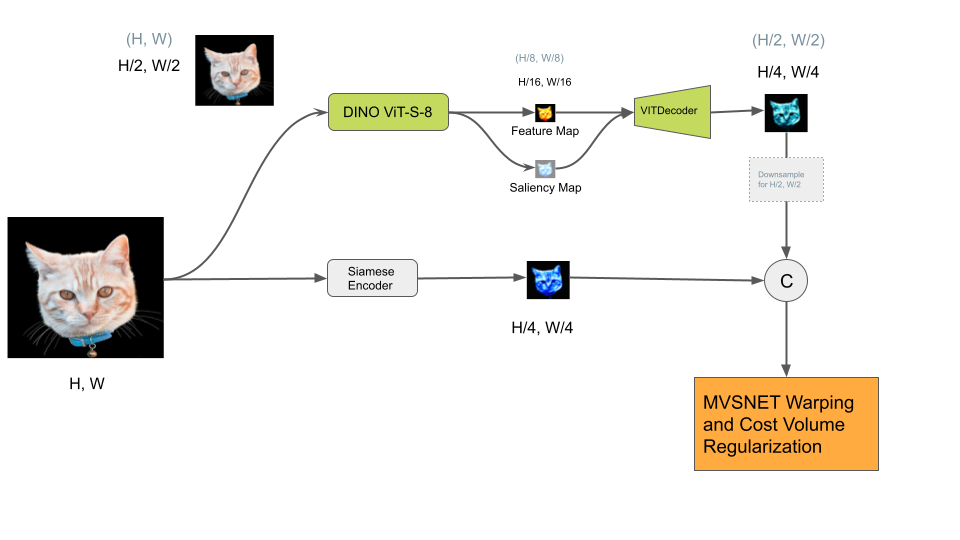
\includegraphics[width=1\textwidth]{images/vit.png}
      \caption[Using ViT features to augment learned features]{\textbf{Using ViT features to augment learned features.} Here, we see how features and saliency maps obtained from the pretrained DINO-ViT-S-8 backbone are used to augment the learned features from {\mvsn} siamese encoder. The final size of the features and saliency maps obtained from the ViT is \(\frac{H}{16}, \frac{W}{16}\). These features and saliency maps are then fused and upscaled to \(\frac{H}{4}, \frac{W}{4}\) by the VITDecoder module\cite{cao2022mvsformer}. For the setting where the ViT feature extractor is given the full-sized images as input (in Grey), we downsample the fused output of the ViTDecoder by a factor of \(\frac{1}{2}\) (shown by the dotted grey rectangle) before concatenating with the learned features from the Siamese encoder.}
\label{fig:vit}
\end{figure}
    
    
    
    \item \textbf{RobustMVD Base: Switching out the DispNet feature encoder in RobustMVD and replacing it with the {\mvsn} encoder.:} Consequently, based on the findings of previous experiments, it is prudent to investigate the impact of replacing the feature encoder in DispNet with the {\mvsn} feature encoder. Our goal was to evaluate whether the distinctive features extracted by {\mvsn}'s encoder would enhance or degrade the performance of DispNet. Initially, the {\mvsn} encoder was incompatible with the DispNet architecture. Therefore, we had to adapt the {\mvsn} encoder for effective integration. Our adaptation involved several significant changes. \par

    Firstly, we increased the initial number of feature channels from 8 to 64. This leads to an increase in the number of channels in the extracted features of the {\mvsn} encoder from 32 to 256. This decision, although initially based on the need to make the {\mvsn} encoder compatible with the rest of the DispNet architecture, also has the added benefit of potentially extracting more complex features from the input images and maintaining the deeper architecture of the {\mvsn} encoder, acknowledging the trade-off of increased computational complexity.\par
    
    Secondly, we adjusted the stride of the first convolutional layer from 1 to 2. This allowed the convolutional filters to skip every other pixel, reducing the output size and computational cost while constructing the correlations and the cost volume. We perform this change to maintain the spatial dimensions of the skip connections from the {\mvsn} encoder to the DispNet decoder. Note that this operation might lead to the loss of some fine-grained detail due to the reduction in input size. \par

    In the original {\mvsn} encoder, every convolution layer uses batch normalization. We changed this in our modified encoder. Specifically, the last convolution layer of each block ($conv1b$, $conv2c$, and $conv3c$ in \hyperref[tab:arch-mvsn]{Table2.1}) was implemented without batch normalization. $conv1b$ and $conv2c$ are fed as skip connections to the decoder part of the cost volume regularization network (refer to \hyperref[tab:arch-mvsn]{Table2.5} for details of the skip connections). Although batch normalization generally improves the speed, performance, and stability of a neural network, we found that, in our case, it led to training divergence. This phenomenon might have been due to the model's increased sensitivity to changes in the distribution of each layer's input, leading to amplified noise or exploding gradients. Therefore, to stabilize our training, we removed it from the last layers. It should be noted that the GC-Net\cite{kendall2017end} architecture also removes BatchNorm and ReLU for the layers whose outputs are used as skip connections to the cost volume regularization network. \par
    
    Another significant modification was removing the $conv3r$ layer from the {\mvsn} encoder. The $conv3r$ layer is initially used to increase the depth of the encoder without changing the spatial dimensions of the output through the use of a 1x1 kernel, potentially facilitating the learning of more complex representations.  It should be noted from \hyperref[tab:arch-rmvd]{Table 3.}{2} that the DispNet architecture has an additional component, the \textit{Context Encoder}, which comes after the feature encoder. It contains a layer, $conv3a_0$, that performs a 1x1 convolution to reduce the depth of the feature map from 256 to 32 while maintaining the spatial dimensions in a similar fashion to the function of the $conv3r$ layer in the original {\mvsn} encoder (refer to \hyperref[tab:arch-mvsn]{Table 2.}{1}). The encoded context obtained from this layer is concatenated to the output of the cost volume fusion layer further down into the network before passing the concatenated tensor to the cost volume regularization layer. By removing the $conv3r$ layer from the original {\mvsn} encoder, we bridged the gap between the two different encoder architectures. We initially tried incorporating the $conv3r$ and the \textit{Context Encoder} in the network. However, including both components led to a divergence in training. Therefore, we removed the final $conv3r$ layer from the {\mvsn} encoder and directly used the output of $conv3c$. \par
    
    During the evaluation, the model trained on {\bms} showed a slight degradation in performance, as seen in \hyperref[tab:feat-enc]{Table 6b.2}. This is counter-intuitive to our expectation of a performance increase given the increase in depth offered by the {\mvsn} encoder and our modification to increase the feature channels from 32 to 256.\par
    We also trained this configuration with {\brs}, and there was a slight performance increase compared to its respective baseline of {\rmvd} trained with {\brs} as seen in \hyperref[tab:feat-enc]{Table 6b.1}. This highlights the sensitivity of the models to the variants of the datasets and batch sizes for training and its consequent effects on the evaluation. We will explore this further in the \hyperref[sec:exp-dataset-prop]{Section 5.3} on the properties of the data and datasets. 


\end{enumerate}

\subsection{Choice of Correlation Layer}\label{subsec:cvc}
In this section, we first take a look at the different types of correlation layers employed in our baseline models as well as in our experiments. We then discuss the results of the experiments in detail.
%\begin{table*}[t!]
\begin{table}[ht!]
\def\arraystretch{1.5}
\begin{adjustbox}{width=1\textwidth}
%\resizebox{\columnwidth}{!}{ % scale to columnwidth
%\resizebox*{\textwidth}{!}{
\setlength{\tabcolsep}{1mm}
\begin{tabular}{|l
|c c
|c c
|c c
|c c
|c c
||c |c |c |c |c
|}

\hline
    \textbf{Correlation Layer w/o}
    & \multicolumn{2}{c|}{\textbf{\kittishort{}}}
    & \multicolumn{2}{c|}{\textbf{\dtushort{}{}}}
    & \multicolumn{2}{c|}{\textbf{\scannetshort{}}}
    & \multicolumn{2}{c|}{\textbf{\tanksandtemplesshort{}}}
    & \multicolumn{2}{c|}{\textbf{\ethdshort{}}}
    & \multicolumn{5}{c|}{\textbf{Average}}
    \\
\hline
    \textbf{Normalized Features}
    & $\absrel\downarrow$ & $\threshI\uparrow$
    & $\absrel\downarrow$ & $\threshI\uparrow$
    & $\absrel\downarrow$ & $\threshI\uparrow$
    & $\absrel\downarrow$ & $\threshI\uparrow$
    & $\absrel\downarrow$ & $\threshI\uparrow$
    & $\absrel\downarrow$ & $\threshI\uparrow$ & AUSE$ \downarrow$ & time $\downarrow$ & memory $\downarrow$
    \\

    &&&&&&&&&&&&&&(mSec)&(MB)\\
    \hline
    \hline

    \textbf{a) {\mvsn} Base}
	& 
	& 
	& 
	& 
	& 
	& 
	& 
	& 
	& 
	& 
	& 
	& 
 	& 
	& 
	& 
    \\
\hline
\rowcolor{bgcolor}
    \textbf{a1) Default Training and}
	& 
	& 
	& 
	& 
	& 
	& 
	& 
	& 
	& 
	& 
	& 
	& 
        & 
	& 
	& 
        \\
\rowcolor{bgcolor}
    \textbf{    Evaluation Input sizes}
	& 
	& 
	& 
	& 
	& 
	& 
	& 
	& 
	& 
	& 
	& 
	& 
        & 
	& 
	& 
        \\
\hdashline
\rowcolor{bgcolor}
	MVSNet Base $(V=2, D=128)$
	& 11.44
	& 40.50
	& 2.95
	& 81.26
	& 9.80
	& 32.31
	& 9.31
	& 80.24
	& 31.45
	& \bestresult{38.51}
	& 12.99
	& \bestresult{55.56}
        & \bestresult{0.26}
        & 65.2
        & 5302
	
	\\ 

\hline
	Groupwise ($G=4$) with
 	& 
	& 
	& 
	& 
	& 
	& 
	& 
	& 
	& 
	& 
	& 
	& 
 	& 
	& 
	& 
	\\ 
        Learned Fusion 
	& 9.90
	& 40.89
	& 3.17
	& \bestresult{81.40}
	& 8.86
	& 33.22
	& \bestresult{6.59}
	& \bestresult{80.80}
	& 21.43
	& 38.06
	& 9.99
	& 54.87
        & 0.27
        & \bestresult{34.23}
        & \bestresult{3153}
	\\ 
\hline
	Groupwise ($G=4$) + WarpOnly
 	& 
	& 
	& 
	& 
	& 
	& 
	& 
	& 
	& 
	& 
	& 
	& 
 	& 
	& 
	& 
	\\ 
        with Learned Fusion 
	& \bestresult{8.17}
	& \bestresult{43.59}
	& 4.01
	& 78.52
	& \bestresult{8.58}
	& \bestresult{34.98}
	& 6.71
	& 80.18
	& \bestresult{19.21}
	& 38.09
	& \bestresult{9.34}
	& 55.07
        & 0.28 
        & 84.28
        & 8527
	\\ 
	
    \hline
    \hline

    \textbf{b) {\rmvd} Base}
	& 
	& 
	& 
	& 
	& 
	& 
	& 
	& 
	& 
	& 
	& 
	& 
 	& 
	& 
	& 
    \\

\hline
\rowcolor{bgcolor}
        \textbf{b1) Train on {\bms}} 
        & 
	& 
	& 
	& 
	& 
	& 
	& 
	& 
	& 
	& 
	& 
	& 
        & 
	& 
	& 
        \\
\rowcolor{bgcolor}
    \textbf{and reduced Evaluation Input sizes}
	& 
	& 
	& 
	& 
	& 
	& 
	& 
	& 
	& 
	& 
	& 
	& 
        & 
	& 
	& 
        \\
\hdashline
\rowcolor{bgcolor}
{\rmvd} Base $(V=2 , B=1)$ \(\star\)
	& \bestresult{8.21}
	& \bestresult{35.51}
	& \bestresult{4.24}
	& \bestresult{71.04}
	& \bestresult{9.06}
	& \bestresult{31.07}
	& 11.34
	& \bestresult{60.78}
	& \bestresult{11.13}
	& \bestresult{36.58}
	& \bestresult{8.80}
	& \bestresult{47.00}
        & 0.28
        & \bestresult{25.23}
        & \bestresult{1136}
	\\ 
    \hline
        Groupwise $(G=4)$ with 
        & 
	& 
	& 
	& 
	& 
	& 
	& 
	& 
	& 
	& 
	& 
	& 
 	& 
	& 
	& 
    \\
	Learned Fusion (600k iterations) 
	& 10.21
	& 30.50
	& 4.92
	& 69.04
	& 38.84
	& 30.21
	& 9.59
	& 55.03
	& 15.29
	& 31.05
	& 15.77
	& 43.16
        & \bestresult{0.26}
        & 64.1
        & 7374
	\\ 
        and 2D cost regularization \(\star\)
	& 
	& 
	& 
	& 
	& 
	& 
	& 
	& 
	& 
	& 
	& 
	& 
 	& 
	& 
	& 
	\\ 
\hline
        Groupwise $(G=4)$ with 
        & 
	& 
	& 
	& 
	& 
	& 
	& 
	& 
	& 
	& 
	& 
	& 
 	& 
	& 
	& 
    \\
	Learned Fusion (1000k iterations)
        & 9.49
	& 30.09
	& 4.38
	& 71.04
	& 39.83
	& 30.14
	& \bestresult{7.37}
	& 56.49
	& 13.89
	& 32.43
	& 14.99
	& 44.04
        & 0.27
        & 61.38
        & 7370
    \\ 
        and 2D cost regularization \(\star\)
	& 
	& 
	& 
	& 
	& 
	& 
	& 
	& 
	& 
	& 
	& 
	& 
 	& 
	& 
	& 
	\\ 
\hline
        Groupwise $(G=4)$ + Full Corr 
	& 
	& 
	& 
	& 
	& 
	& 
	& 
	& 
	& 
	& 
	& 
	& 
 	& 
	& 
	& 
	\\ 
        with Learned fusion and
	& 32.21
	& 12.91
	& 5868.07
	& 0
	& 2061.13
	& 0.63
	& 96.27
	& 14.69
	& 795.89
	& 5.01
	& 1770.71
	& 6.65
        & 0.35
        & 127.32
        & 7504
	\\ 
         3D cost regularization \(\star\)
        & 
	& 
	& 
	& 
	& 
	& 
	& 
	& 
	& 
	& 
	& 
	& 
 	& 
	& 
	& 
	\\ 

	
\hline




	

\end{tabular}
\end{adjustbox}
\caption[Changing the correlation layer]{\textbf{Changing the correlation layer}.
\textbf{a)} All {\mvsn} and {\rmvd} derivatives are trained on {\bms}. In \textbf{a.1}, we can see that both implementations with {\gwc} (GWC) and the GWC combined with differential homography outperform the baseline. The model using only GWC as a correlation layer has a significantly lesser inference time and memory requirement. In \textbf{b.1}, all our implemented models for {\rmvd} using GWC perform very poorly compared to the baseline. Due to the high memory requirements of GWC for {\rmvd} due to 256 channels in the feature maps, we use the smaller evaluation inputs. This is indicated by a \(\star\). The baselines are shaded in grey.
\label{tab:corr-layer}
}
\end{table}

%\end{table*}

\begin{enumerate}
    \item \textbf{Plane sweep based Warping}\cite{Yao2018}: As the name suggests, this is not really a correlation operation. This operation was used first in {\mvsn} and later in some of its extensions \cite{Gu2020, yang2019hierarchical, Yao2019} to warp the source features to the reference image frustum at different depth levels and build a cost volume. Consequently, these methods also use a variance-based cost volume fusion methodology, which looks at the variance between the warped source features and the reference features. We saw the working of this in \hyperref[sec:multiviewster]{Section 4} of the Background chapter. 
    \item \textbf{Full Correlation} \cite{Mayer2016}: The Full Correlation, was introduced for the first time in the DispNet paper. The Full correlation is computed as per the following equation.
    \begin{equation}
        c(\mathcal{F}_{ref}, \mathcal{F}_{source}) = \langle \mathcal{F}_{ref} , \mathcal{F}_{source}^T \rangle
    \end{equation} where $\langle:,:\rangle$ denotes matrix multiplication.
    This operation contains  \(C \times W^2\times H^2\) multiplications, is computationally intensive, and is performed for each pair of source and reference images. Here \(C\) is the number of channels in the feature maps of the reference and source images. We can see that this operation decimates the feature dimension of the two feature maps. The correlation map has dimensions ($B \times (W\times H) \times (W\times H)$). It contains matching similarity costs between the key view pixels and points on their respective epipolar lines in the source view for a set of sampled inverse depth values. The individual correlation maps are then fused together with a learned weights fusion or simply averaging them together. {\rmvd} uses this correlation method to obtain a 2D cost map. 
    \item \textbf{{\gwc}} \cite{guo2019group}: {\gwc} (GWC) was first used by Guo {\etal} to calculate the similarity between the left and right images in stereo matching by disparity estimation. This thesis extends it to the depth estimation with the MVS scenario. After the initial warping step, we the source features warped at each depth level with a projection of the reference features along the depth of the frustum. Unlike traditional correlation, which calculates the similarity between pixels along all feature channels, {\gwc} considers a group of channels simultaneously. The {\gwc} volume is computed as follows: 
    \begin{enumerate}
        \item Given the warped and projected source and projected reference features of dimensions \((B, C, D, H, W)\), we reshape them into tensors of shape \((B, G, \frac{C}{G}, D, H, W)\). Here, \(G\) is the number of groups. 
        \item We then take an element-wise inner product between the reshaped tensors and sum over the \(\frac{C}{G}\) or the group-channels dimension.
        \item The cost volume obtained \(V_{gwc}\) has a shape \((B, G, D, H, W)\) and is given as: 

            \[V_{gwc} =\Sigma_{group-channels} (A \odot B)\]

        where $A$ is the reference feature and \(B\) is the warped source feature projected along the depth of the frustum. And \(\odot\) represents the element-wise inner product. The summation operation is performed along the \(\frac{C}{G}\) dimension after taking the product. We used learned fusion to fuse the individual cost volumes. 
    \end{enumerate}
\end{enumerate}
It should be noted that since the correlation layer and the subsequent fusion operation are the most defining parts of an {\mvs} pipeline, we do not switch the full correlation and the differential homography between {\rmvd} and {\mvsn}. Instead, we perform two different types of experiments. In the first type, we replace the existing correlation layer with {\gwc} and use learned fusion to fuse the individual pairwise cost volumes while retaining the remaining architecture as it is. In the second type, we concatenate the output of the original correlation layer of the model with the output of the {\gwc} and use learned fusion to fuse the concatenated volumes. The fused volume is then given as input to either a 3D or 2D cost volume regularization network. \par

For our experiments, we set the value of \(G\) to 4. From \hyperref[tab:corr-layer]{Table 7a.}{1}, we can see that {\gwc} outperforms our {\mvsn} baseline by a significant margin. We also implemented a {\mvsn} multi-correlation model that computes both plane sweep warping volume and {\gwc} volume for each reference and source pair. We then concatenate both volumes and fuse the individual concatenated volumes using learned fusion by computing the weights for each concatenated volume. This model outperforms both the baseline and the model with only {\gwc}. 

For {\rmvd}, it should be noted that the models are trained on the {\bms}, which contains two best views and a batch size of 1. In \hyperref[tab:corr-layer]{Table 7b.}{1}, we observe a significant reduction in performance compared to the respective baseline. We include an additional layer to the architecture called the \textit{CostVolume3DContextEncoder}. This contains three 3D convolutional layers, each with a kernel size of one, to reduce the number of channels in \(V_{gwc}\) from \(G\) to 1. We then squeezed the channel dimension and used the 2D DispNet cost volume regularization network to regress the depth and the uncertainty maps from this reduced cost volume. We conjectured that the model needed more time to learn the additional weights, so we trained it for 1000000 iterations instead of the usual 600000. We observed a slight improvement in performance for the model that was trained for a longer period; however, it was not enough to justify the continuation of training. \par

The third experiment for {\rmvd} consists of the concatenation of the output of the {\gwc} operation and the Full correlation operation. Since the full correlation output does not have an explicit channel dimension, we unsqueeze the tensor at the first dimension and concatenate it to the output of the GWC layer. We further concatenate the output of the context encoder unit of the {\rmvd} model (refer to \hyperref[tab:arch-rmvd]{Table 3.}{2}) to this by expanding it along the depth dimension. This concatenated tensor is then passed on to the 3D cost volume regularization network. In \hyperref[tab:corr-layer]{Table 7b.}{1} in the third entry, we can see that this model performs very poorly compared to the baseline and the other implemented models. 
\subsection{Choice of Cost Volume Fusion Method}\label{subsec:cvf}
%\begin{table*}[t!]
\begin{table}[ht!]
\def\arraystretch{1.5}
\begin{adjustbox}{width=1\textwidth}
%\resizebox{\columnwidth}{!}{ % scale to columnwidth
%\resizebox*{\textwidth}{!}{
\setlength{\tabcolsep}{1mm}
\begin{tabular}{|l
|c c
|c c
|c c
|c c
|c c
||c |c |c |c |c
|}

\hline

    \textbf{Fusion Method}
    & \multicolumn{2}{c|}{\textbf{\kittishort{}}}
    & \multicolumn{2}{c|}{\textbf{\dtushort{}{}}}
    & \multicolumn{2}{c|}{\textbf{\scannetshort{}}}
    & \multicolumn{2}{c|}{\textbf{\tanksandtemplesshort{}}}
    & \multicolumn{2}{c|}{\textbf{\ethdshort{}}}
    & \multicolumn{5}{c|}{\textbf{Average}}
    \\
\hline
    & $\absrel\downarrow$ & $\threshI\uparrow$
    & $\absrel\downarrow$ & $\threshI\uparrow$
    & $\absrel\downarrow$ & $\threshI\uparrow$
    & $\absrel\downarrow$ & $\threshI\uparrow$
    & $\absrel\downarrow$ & $\threshI\uparrow$
    & $\absrel\downarrow$ & $\threshI\uparrow$ & AUSE$ \downarrow$ & time $\downarrow$ & memory $\downarrow$
    \\

    &&&&&&&&&&&&&&(mSec)&(MB)\\
    \hline
    \hline

    \textbf{a) {\mvsn} Base}
	& 
	& 
	& 
	& 
	& 
	& 
	& 
	& 
	& 
	& 
	& 
	& 
 	& 
	& 
	& 
    \\
    \hline
    \rowcolor{bgcolor}
    \textbf{a1) Default Training and}
	& 
	& 
	& 
	& 
	& 
	& 
	& 
	& 
	& 
	& 
	& 
	& 
        & 
	& 
	& 
        \\
\rowcolor{bgcolor}
    \textbf{    Evaluation Input sizes}
	& 
	& 
	& 
	& 
	& 
	& 
	& 
	& 
	& 
	& 
	& 
	& 
        & 
	& 
	& 
        \\
\hdashline
\rowcolor{bgcolor}
	MVSNet Base $(V=2, D=128)$
	& \bestresult{11.44}
	& \bestresult{40.50}
	& \bestresult{2.95}
	& \bestresult{81.26}
	& \bestresult{9.80}
	& \bestresult{32.31}
	& \bestresult{9.31}
	& \bestresult{80.24}
	& \bestresult{31.45}
	& \bestresult{38.51}
	& \bestresult{12.99}
	& \bestresult{55.56}
        & \bestresult{0.26}
        & 65.2
        & 5302
	
	\\ 

\hline
	{\mvsn} with Learned Fusion
	& 27.53
	& 10.48
	& 9.71
	& 49.54
	& 15.52
	& 17.25
	& 12.73
	& 50.88
	& 38.42
	& 16.50
	& 20.78
	& 28.93
        & 0.39
        & 37.21
        & 5732
	\\ 
 \hline
	{\mvsn} with Average Fusion
	& 37.42
	& 10.44
	& 9.29
	& 48.40
	& 16.91
	& 18.91
	& 14.28
	& 47.44
	& 40.21
	& 14.36
	& 22.06
	& 27.87
        & 0.37
        & \bestresult{35.82}
        & \bestresult{4322}
	\\

\hline
\hline
        \textbf{b){\rmvd} Base}
	& 
	& 
	& 
	& 
	& 
	& 
	& 
	& 
	& 
	& 
	& 
	& 
 	& 
	& 
	& 
	\\
 \hline
 \rowcolor{bgcolor}
        \textbf{b1) Train on {\bms}} 
        & 
	& 
	& 
	& 
	& 
	& 
	& 
	& 
	& 
	& 
	& 
	& 
        & 
	& 
	& 
        \\
\rowcolor{bgcolor}
    \textbf{and default Evaluation Input sizes}
	& 
	& 
	& 
	& 
	& 
	& 
	& 
	& 
	& 
	& 
	& 
	& 
        & 
	& 
	& 
        \\
\hdashline
\rowcolor{bgcolor}
{\rmvd} Base $(V=2 , B=1)$ 
	& \bestresult{8.22}
	& \bestresult{35.51}
	& 4.74
	& 68.00
	& 9.06
	& 31.07
	& 12.58
	& 62.87
	& \bestresult{11.58}
	& 36.60
	& 9.24
	& 46.81
        & 0.28
        & \bestresult{30.24}
        & 2125
	\\ 
 \hline
        {\rmvd} with Average Fusion \((V=2)\)
	& 8.99
	& 34.82
	& \bestresult{4.06}
	& \bestresult{73.66}
	& \bestresult{8.83}
	& \bestresult{31.68}
	& \bestresult{9.91}
	& \bestresult{65.65}
	& 13.34
	& \bestresult{39.16}
	& \bestresult{9.02}
	& \bestresult{48.99}
        & \bestresult{0.26}
        & 45.53
        & \bestresult{1783}
	\\ 
	


	
\hline
\end{tabular}
\end{adjustbox}
\caption[Changing the cost volume fusion layer]{\textbf{Changing the cost volume fusion layer}.
\textbf{a)} For experiments with the fusion layer, both {\mvsn} derivatives and {\rmvd} derivatives are trained on {\bms}. A variance-based fusion only makes sense if there is only warping and no correlation computation between the reference and source features, as in {\mvsn}. In \textbf{a.1}, we can see that both learned fusion and average fusion don't work well with {\mvsn} for this reason. Consequently, we omit the combination {\rmvd} with Variance Fusion because {\rmvd} computes the full correlation between the reference and the source features. In \textbf{b.1}, we can see that average fusion gives slightly better results for average fusion compared to learned fusion for the given number of views. It should be noted that this might not necessarily be the case if the same experiment is repeated with a larger number of source views. 
\label{tab:cvf}
}
\end{table}

%\end{table*}

\begin{enumerate}
    \item \textbf{Variance Fusion} \cite{Yao2018}: This is used in the baseline {\mvsn} model. Variance-based fusion of individual cost volumes operates on the principle that all views contribute equally to the final fused cost volume. A cost metric based on variance is only applicable in models that utilize a differential homography warping approach, as correlation computation between reference and source features is not explicitly performed during the homography warping process.\hyperref[tab:arch-mvsn]{Table 2.3} gives the equation to obtain the fused cost volume from the individual cost volumes. We only use variance-based fusion for some {\mvsn} derivatives that only warp the source features to the reference features, as the cost volumes generated by any model that computes correlations cannot be fused with a variance metric. Hence, we cannot fuse the full correlations of {\rmvd} with variance fusion.  
    \item \textbf{Learned Fusion}\cite{schroeppel2022benchmark, Hartmann2017}: In learned fusion, we pass the individual cost volumes through a small 2D or 3D CNN network to learn the respective weights for each volume. First, we utilize the per-pixel (for 2D cost maps) or voxel weights (for 3D cost volumes) that we acquired. We applied these weights to each individual volume and then calculated a weighted average to produce the final fused cost volume. Unlike the variance operation, learned fusion can be used for derivatives of {\mvsn} that employ a different correlation layer other than the differential warping and {\rmvd}. Therefore, as part of our ablation study, we implemented {\mvsn} with learned fusion. In \hyperref[tab:cvf]{Table 8a.1}, we can see that the learned fusion for {\mvsn} performed much worse than the variance-based fusion baseline. This is because variance-based fusion implicitly computes the similarity between reference and individual warped source volumes instead of explicitly computing the correlation between the two. Hence, learned fusion does not work well in such a scenario, with no actual matching costs in the cost volume. We used learned fusion extensively in our models, where the correlation is computed explicitly in the correlation layer, such as the {\mvsn} models using {\gwc} as a correlation layer in the previous section. 
    \item \textbf{Average Fusion}\cite{im2019dpsnet}: Average fusion, like learned fusion, can be used for both {\mvsn} and {\rmvd} models. In \hyperref[tab:cvf]{Table 8a.1}, we can see the performance is slightly worse than the learned fusion for {\mvsn} and significantly worse than the baseline based on variance fusion. In \hyperref[tab:cvf]{Table 8b.1} {\rmvd} with average fusion performs slightly better than our baseline model, which uses a learned fusion strategy. Schröppel \etal demonstrates this by training {\rmvd} with average fusion using four views instead of two. This model exhibits a slightly lower performance than the baseline {\rmvd} model trained with learned fusion. \cite{schroeppel2022benchmark}
\end{enumerate}
\subsection{Choice of Cost Volume Regularization Network Component}\label{subsec:cvr}
%\begin{table*}[t!]
\begin{table}[ht!]
\footnotesize
\centering
\def\arraystretch{1.5}
%\resizebox{\columnwidth}{!}{ % scale to columnwidth
%\resizebox*{\textwidth}{!}{
\begin{adjustbox}{width=1\textwidth}
\setlength{\tabcolsep}{1mm}
\begin{tabular}{|l
|c c
|c c
|c c
|c c
|c c
||c |c |c |c |c
|}

\hline

    \textbf{Cost Vol Regularization}
    & \multicolumn{2}{c|}{\textbf{\kittishort{}}}
    & \multicolumn{2}{c|}{\textbf{\dtushort{}{}}}
    & \multicolumn{2}{c|}{\textbf{\scannetshort{}}}
    & \multicolumn{2}{c|}{\textbf{\tanksandtemplesshort{}}}
    & \multicolumn{2}{c|}{\textbf{\ethdshort{}}}
    & \multicolumn{5}{c|}{\textbf{Average}}
    \\
\hline
    & $\absrel\downarrow$ & $\threshI\uparrow$
    & $\absrel\downarrow$ & $\threshI\uparrow$
    & $\absrel\downarrow$ & $\threshI\uparrow$
    & $\absrel\downarrow$ & $\threshI\uparrow$
    & $\absrel\downarrow$ & $\threshI\uparrow$
    & $\absrel\downarrow$ & $\threshI\uparrow$ & AUSE$ \downarrow$ & time $\downarrow$ & memory $\downarrow$
    \\
    &&&&&&&&&&&&&&(mSec)&(MB)\\
    \hline
    \hline
    \textbf{a) {\mvsn} Base}
	& 
	& 
	& 
	& 
	& 
	& 
	& 
	& 
	& 
	& 
	& 
	& 
 	& 
	& 
	& 
    \\
\hline
    \rowcolor{bgcolor}
    \textbf{a1) Default Training and}
	& 
	& 
	& 
	& 
	& 
	& 
	& 
	& 
	& 
	& 
	& 
	& 
        & 
	& 
	& 
        \\
\rowcolor{bgcolor}
    \textbf{    Evaluation Input sizes}
	& 
	& 
	& 
	& 
	& 
	& 
	& 
	& 
	& 
	& 
	& 
	& 
        & 
	& 
	& 
        \\
\hdashline
\rowcolor{bgcolor}
	MVSNet Base $(V=2, D=128)$
	& 11.44
	& 40.50
	& 2.95
	& 81.26
	& 9.80
	& 32.31
	& 9.31
	& 80.24
	& 31.45
	& 38.51
	& 12.99
	& 55.56
        & 0.26
        & 65.2
        & \bestresult{5302}
	
	\\ 

\hline
	DispNet 2D Decoder 
	& \bestresult{7.79}
	& \bestresult{48.92}
	& 2.83
	& 83.22
	& \bestresult{8.20}
	& \bestresult{36.84}
	& \bestresult{5.75}
	& \bestresult{83.76}
	& \bestresult{19.26}
	& \bestresult{40.63}
	& \bestresult{8.77}
	& \bestresult{58.67}
        & 0.29
        & 627.45
        & 5491
	\\ 
\hline
     3D UNet Stacked Hourglass
	& 10.63
	& 39.58
	& \bestresult{2.64}
	& \bestresult{85.33}
	& 9.96
	& 32.90
	& 6.13
	& 81.82
	& 25.73
	& 38.31
	& 11.02
	& 55.59
        & \bestresult{0.25}
        & \bestresult{45.54}
        & 5373
    \\
	



\hline
\end{tabular}
\end{adjustbox}
\caption[Changing the cost volume regularization layer]{\textbf{Changing the cost volume regularization layer}.
\textbf{a)} All {\mvsn} derivatives are trained on {\bms}. It is evident that both of our models outperform the baseline. Particularly, the implementation of {\mvsn} using a 2D DispNet decoder shows significant improvement over the baseline. However, we can see that it takes significantly longer to make inferences compared to the baseline. In the second entry, we see that applying the Stacked Hourglass regularization yields better results than the baseline without causing a significant increase in inference time and memory requirements.
\label{tab:cvr}
}
\end{table}

%\end{table*}

\begin{enumerate}
    \item \textbf{Switching out the MVSNet fused cost-volume decoder with the DispNet fused cost-volume decoder.:} In the original MVSNet, the cost volume is a 3D volume with dimensions (Batch size, Channels, Depth levels, Height, Width). Here, each pixel across all depth planes is associated with a probability of that pixel at that depth being part of the object surface in the scene. It is a structured cost volume that is then passed to a 3D CNN Encoder Decoder cost volume regularization component. Now, since we wanted to switch to the DispNet cost volume decoder, which is a 2D decoder, we deal with this problem by slicing the fused cost volume along the depth dimension in a similar fashion to \cite{Yao2019}. \par
    
    The simplest way to integrate the 3D fused cost volume into a 2D decoder is to slice it at each depth level and pass each layer individually to the 2D decoder. The output of each layer could then be interpreted as a probability map for that depth. The depth map can then be obtained by choosing the depth with the maximum probability for each pixel. However, this increases the time complexity, as the 2D decoder needs to process the image once for each depth layer. \par
    The skip connections from the fused cost volume encoder are also three-dimensional. However, since they are intermediary representations, they have a larger number of depth levels compared to the final output of the cost volume encoder. To reconcile this difference, we use trilinear interpolation to match the slices from intermediate volumes with fewer depth dimensions, including the final output, to those of the output with the largest depth dimension, which in our case is $3DConv0$. For instance, given that we have volumes of sizes (1, 64, 32, 4, 5) and (1, 32, 64, 8, 10), we interpolate along the depth dimension of the first volume to match the depth dimension of the second volume, which gives the new volume of shape (1, 64, 64, 4, 5). \par
    To preserve the spatial correlation between the slices, we maintain the order of the slices along the depth dimension, as it represents the spatial relationship between different depths. In this manner, we use the 3D skip connections in the 2D decoder by transforming the 3D volumes into a series of individual 2D depth planes, which we then feed into the 2D decoder at the appropriate layers. This process is visualized in \hyperref[fig:2ddec-3dcv]{Figure 6}.\par
    \begin{figure}[ht]
    \centering
     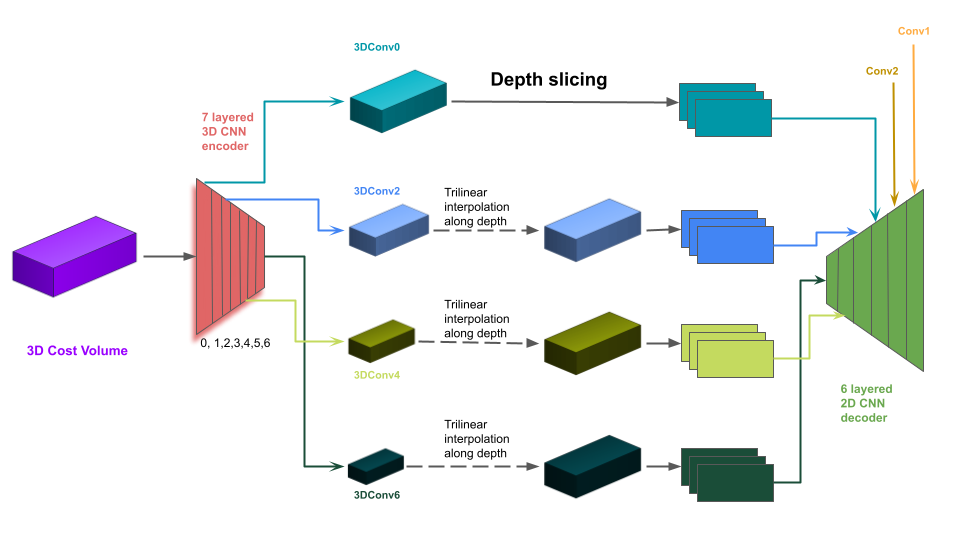
\includegraphics[width=1\textwidth]{images/2ddec-3dcv.png}
      \caption[Using a 2D Decoder for 3D Cost Volume Regularization]{\textbf{Using a 2D Decoder for 3D Cost Volume Regularization.} This figure shows the method of \textit{depth slicing} used to regularize a 3D cost volume using a 3D-2D hybrid Encoder-Decoder. The final and intermediate skip connection outputs of the 3D encoder are interpolated along the depth dimension to match the number of depth levels in each of them. Then, each \textit{depth slice} of the final encoder output, along with its corresponding depth slices from the intermediate representations, are sent individually to the 2D decoder for processing. The decoder outputs from each tuple of \textit{depth slices} are then stacked along the depth dimension, and the depth map is regressed from this cost volume. This final step is not shown in the figure.}
    \label{fig:2ddec-3dcv}
    \end{figure}
    This method takes longer to train than a normal 3D convolution decoder, as the decoder is called for each tuple of depth slices. These tuples look like ($3Dconv0[:,:,i,:,:]$, $3Dconv2[:,:,i,:,:]$, $3Dconv4[:,:,i,:,:]$, $3Dconv6[:,:,i,:,:]$). The maximum value of $i$ depends on the number of depth sampling points chosen at the beginning of the training, which in our case is $D=128$. In \hyperref[tab:cvr]{Table 9a.1}, we can see that this model gives much better results compared to the baseline of training {\mvsn} on {\bms} with $128$ depth samples. It also performs better than training {\mvsn} with $256$ depth values. The drawback of this model is that it takes a long time to train because each depth slice is processed by the cost volume decoder individually. The output of each iteration is aggregated into a new regularized cost volume along the depth dimension. The final depth map is regressed from this cost volume.\par 

    \item \textbf{{\mvsn} with Stacked Hourglass Cost Volume Regularization Network}: In this experiment, we implemented a stacked hourglass network, which is used for regularizing the raw fused cost volume. The architecture for this network is given in detail in \hyperref[tab:arch-stacked]{Table 16}{}. Each \textit{hourglass} in the architecture is an encoder-decoder network with skip connections going from the encoder to the decoder. Our architecture incorporates three distinct hourglass modules. After every level, a depth map is generated from the probability volume. To calculate the loss, we use a weighted summation of the smooth L1 loss between the depth maps and ground truth at each output level of the stacked hourglass. From \hyperref[tab:cvr]{Table 9a.1}, we can see that this model also performs better than the baseline without significantly increasing inference time and memory requirement. 

\end{enumerate}



\subsection{Usage of Coarse to Fine Architecture} \label{subsec:c2f}
For the experiments in this section, we re-engineered our baseline models in a coarse-to-fine design \cite{Gu2020}. We consider a three-stage design. The depth range in the first stage, \(R_1\), encompasses the entire depth range of the input scene. Subsequent stages use the previously predicted output to constrict this initial hypothesized range. Mathematically, this is given by \(R_{k+1} = R_k \times w_k\), where \(R_k\) is the hypothesis range at stage \(k\) and \(w_k < 1\) is the reduction factor. Similarly, the depth interval at the initial stage is symbolized as \(I_1\). This interval is relatively larger than that in conventional singular cost volume formulations used in our baselines, making the primary depth estimation coarser. For subsequent stages, we use narrower intervals to derive finer-grained outputs. This can be written as \(I_{k+1} = I_k \times p_k\), where \(I_k\) is the hypothesis plane interval during the \(k^{th}\) stage and \(p_k < 1\) is the decrement factor. For stage \(k\), the total number of hypothesis planes, \(D_k\), is computed as \(D_k = \frac{R_k}{I_k}\). We use a value of \(p_k =\frac{1}{2}\). We use [32, 16, 8] depth hypotheses from the coarsest to the finest level. The interval ratios are set to [4, 2, 1]. This is such that the product of the interval ratio and the number of depth hypotheses at the coarsest level $32\times4=128$, which is equal to the number of depth hypotheses that we use for a single stage {\mvsn} model\cite{Gu2020}. The cascade formulation reduces the overall count of hypothesis planes as we refine the initial depth range in subsequent stages. Similar to \hyperref[eq:homography]{Equation 11}, the homography warping function for the \(k + 1^{th}\) stage can be reformulated as:
\begin{equation}
H_i(d^m_k + \Delta^m_{k+1}) = K_i \cdot R_i \cdot (I - \frac{(t_1 - t_i) \cdot n^T_1}{d^m_k + \Delta^m_{k+1}}) \cdot R^T_1 \cdot K^{-1}_1 \cdot d^m_k
\end{equation}
Here, \(d^m_k\) stands for the predicted depth of pixel \(m\) during the \(k^{th}\) stage, while \(\Delta^m_{k+1}\) represents the \(m^{th}\) pixel's residual depth for the \(k + 1^{th}\) stage\cite{zhu2021deep}.

We used the same smooth \(l1\) loss here as we did for our baselines with a slight modification. The predicted depth maps of each stage \(k\) are weighted by a factor \(\lambda_k\), and the total loss is the sum of all weighted losses. \par

In this section, we examine the impact of changing the feature extractors on the performance of models for coarse-to-fine design. Generating multilevel features is the most crucial component, so we focus on this. We trained the models using two different feature extractors: FPN and UNet. Unlike the FPN in \hyperref[subsec:fe]{Section 5.2.1}, we use a stride of one in the first $conv1a$ layer. Thus, the feature maps at each level have twice the resolution of the feature maps from the other implementation of FPN. These resolutions are given in \hyperref[tab:arch-fpn]{Table 13} in red. Similarly, for the UNet, we use all the features starting from \(feat2\) at the coarsest level and \(feat0\) at the finest level. This is possible due to the reduced number of depth hypotheses used in a coarse-to-fine architecture. 
Our experiments yielded results that are outlined in \hyperref[tab:c2f]{Table 10}. We observed that the {\mvsn} coarse-to-fine model with FPN feature extractor outperformed the baseline and had a much lower memory requirement, albeit requiring slightly more time for training and inference. This might be attributed to the adaptive number of depth levels and the cascading design of depth refinement. However, the UNet feature extractor-based coarse-to-fine design performed poorly compared to the baseline. Therefore, we can conclude that the FPN feature extractor is more suitable for a coarse-to-fine scenario than the UNet.

%\begin{table*}[t!]
\begin{table}[ht!]
\footnotesize
\centering
\def\arraystretch{1.5}
\begin{adjustbox}{width=1\textwidth}
%\resizebox{\columnwidth}{!}{ % scale to columnwidth
%\resizebox*{\textwidth}{!}{
\setlength{\tabcolsep}{1mm}
\begin{tabular}{|l
|c c
|c c
|c c
|c c
|c c
||c |c |c |c |c
|}

\hline

    \textbf{Feature Extractor for}
    & \multicolumn{2}{c|}{\textbf{\kittishort{}}}
    & \multicolumn{2}{c|}{\textbf{\dtushort{}{}}}
    & \multicolumn{2}{c|}{\textbf{\scannetshort{}}}
    & \multicolumn{2}{c|}{\textbf{\tanksandtemplesshort{}}}
    & \multicolumn{2}{c|}{\textbf{\ethdshort{}}}
    & \multicolumn{5}{c|}{\textbf{Average}}
    \\
\hline
    \textbf{Coarse-to-Fine}
    & $\absrel\downarrow$ & $\threshI\uparrow$
    & $\absrel\downarrow$ & $\threshI\uparrow$
    & $\absrel\downarrow$ & $\threshI\uparrow$
    & $\absrel\downarrow$ & $\threshI\uparrow$
    & $\absrel\downarrow$ & $\threshI\uparrow$
    & $\absrel\downarrow$ & $\threshI\uparrow$ & AUSE$ \downarrow$ & time $\downarrow$ & memory $\downarrow$
    \\

    &&&&&&&&&&&&&&(mSec)&(MB)\\
    \hline
    \hline
    \textbf{a) {\mvsn} Base}
	& 
	& 
	& 
	& 
	& 
	& 
	& 
	& 
	& 
	& 
	& 
	& 
 	& 
	& 
	& 
    \\
\hline
    \rowcolor{bgcolor}
    \textbf{a1) Default Training and}
	& 
	& 
	& 
	& 
	& 
	& 
	& 
	& 
	& 
	& 
	& 
	& 
        & 
	& 
	& 
        \\
\rowcolor{bgcolor}
    \textbf{    Evaluation Input sizes}
	& 
	& 
	& 
	& 
	& 
	& 
	& 
	& 
	& 
	& 
	& 
	& 
        & 
	& 
	& 
        \\
\hdashline
\rowcolor{bgcolor}
	MVSNet Base $(V=2, D=128)$
	& \bestresult{11.44}
	& \bestresult{40.50}
	& \bestresult{2.95}
	& \bestresult{81.26}
	& 9.80
	& 32.31
	& 9.31
	& 80.24
	& 31.45
	& \bestresult{38.51}
	& 12.99
	& \bestresult{55.56}
        & \bestresult{0.26}
        & \bestresult{65.2}
        & 5302
	
	\\ 
 \hline
	Cascade {\mvsn} with FPN FE
	& 16.11
	& 26.53
	& 3.31
	& 79.77
	& \bestresult{9.66}
	& 33.42
	& \bestresult{5.83}
	& \bestresult{81.55}
	& \bestresult{19.78}
	& 37.34
	& \bestresult{10.94}
	& 51.72
        & 0.88
        & 168.31
        & 2101
	\\ 
 \hline
	Cascade {\mvsn} with UNet FE
	& 24.15
	& 23.94
	& 3.21
	& 79.90
	& 10.20
	& \bestresult{33.69}
	& 7.66
	& 80.14
	& 25.85
	& 36.54
	& 14.22
	& 50.84
        & 0.86
        & 154.31
        & \bestresult{2044}
	\\

	
\hline
\end{tabular}
\end{adjustbox}
\caption[Changing the feature extractor for Coarse-to-Fine model design]{\textbf{Changing the feature extractor for Coarse-to-Fine model design}.
\textbf{a)}All {\mvsn} derivatives are trained on {\bms}. From the results, it is evident that the {\mvsn} coarse-to-fine model with FPN feature extractor outperforms the baseline. On the other hand, the model that has the UNet feature extractor performs poorly. Both models have a higher degree of uncertainty than the baseline and take longer to make inferences. However, the memory requirements for these models are significantly lower.
\label{tab:c2f}
}
\end{table}

%\end{table*}



\section{Effects of Changing Training Dataset Properties}\label{sec:exp-dataset-prop}
In this section, we analyze how modifying the properties of the input data impacts the model's performance. We do not make any changes to the test input data. All other settings are kept constant, and only a single attribute is changed in each experiment. All {\mvsn} models are given the camera intrinsics, poses, and depth range as input. All {\rmvd} models are given only the camera intrinsics and the poses as inputs. We do this to maintain similarity with the respective baselines. All {\rmvd} models are trained with Scale Augmentation unless explicitly specified. 
%\begin{table*}[t!]
\begin{table}[ht!]
\footnotesize
\centering
\def\arraystretch{1.5}
\begin{adjustbox}{width=1\textwidth}
%\resizebox{\columnwidth}{!}{ % scale to columnwidth
%\resizebox*{\textwidth}{!}{
\setlength{\tabcolsep}{1mm}
\begin{tabular}{|l
|c c
|c c
|c c
|c c
|c c
||c |c |c |c |c
|}

\hline

    \textbf{Approach}
    & \multicolumn{2}{c|}{\textbf{\kittishort{}}}
    & \multicolumn{2}{c|}{\textbf{\dtushort{}{}}}
    & \multicolumn{2}{c|}{\textbf{\scannetshort{}}}
    & \multicolumn{2}{c|}{\textbf{\tanksandtemplesshort{}}}
    & \multicolumn{2}{c|}{\textbf{\ethdshort{}}}
    & \multicolumn{5}{c|}{\textbf{Average}}
    \\
\hline
    & $\absrel\downarrow$ & $\threshI\uparrow$
    & $\absrel\downarrow$ & $\threshI\uparrow$
    & $\absrel\downarrow$ & $\threshI\uparrow$
    & $\absrel\downarrow$ & $\threshI\uparrow$
    & $\absrel\downarrow$ & $\threshI\uparrow$
    & $\absrel\downarrow$ & $\threshI\uparrow$ & AUSE$ \downarrow$ & time $\downarrow$ & memory $\downarrow$
    \\

    &&&&&&&&&&&&&&(mSec)&(MB)\\
    \hline
    \hline

    \textbf{a) Change Dataset}
	& 
	& 
	& 
	& 
	& 
	& 
	& 
	& 
	& 
	& 
	& 
	& 
 	& 
	& 
	& 
    \\
\hline
\rowcolor{bgcolor}
    \textbf{a1)} {\mvsn} Baseline \((V=2, D=128)\)
	& \bestresult{11.44}
	& \bestresult{40.50}
	& 2.95
	& 81.26
	& \bestresult{9.80}
	& \bestresult{32.31}
	& 9.31
	& \bestresult{80.24}
	& 31.45
	& \bestresult{38.51}
	& \bestresult{12.99}
	& \bestresult{55.56}
        & 0.26
        & \bestresult{65.2}
        & \bestresult{5302}
    \\
\hline
	{\mvsn} trained on {\dtushort{}{}} 
        & 
	& 
	& 
	& 
	& 
	& 
	& 
	& 
	& 
	& 
	& 
	& 
 	& 
	& 
	& 
    \\

        ($D=128, V=2$)
	& 18.67
	& 38.80
	& \bestresult{2.32}
	& \bestresult{85.84}
	& 12.17
	& 26.55
	& \bestresult{8.28}
	& 75.35
	& \bestresult{26.44}
	& 31.98
	& 13.57
	& 51.70
        & -
        & 112.73
        & 8716
	\\ 
    \hline
    \rowcolor{bgcolor}
        \textbf{a2)} {\rmvd} Baseline with
        & 
	& 
	& 
	& 
	& 
	& 
	& 
	& 
	& 
	& 
	& 
	& 
 	& 
	& 
	& 
    \\
\rowcolor{bgcolor}
    {\bms} \((V=2)\)
 	& \bestresult{8.22}
	& \bestresult{35.51}
	& 4.74
	& \bestresult{68.00}
	& \bestresult{9.06}
	& \bestresult{31.07}
	& \bestresult{12.58}
	& \bestresult{62.87}
	& \bestresult{11.58}
	& \bestresult{36.60}
	& \bestresult{9.24}
	& \bestresult{46.81}
        & 0.28
        & 30.24
        & 2125
    \\
    \hline
        {\rmvd} trained on {\dtushort{}{}} 
	& 
	& 
	& 
	& 
	& 
	& 
	& 
	& 
	& 
	& 
	& 
	& 
 	& 
	& 
	& 
	\\ 

        ($D=256, V=2$)
	& 48.16
	& 4.07
	& \bestresult{3.82}
	& 62.39
	& 33.70
	& 5.98
	& 50.80
	& 10.71
	& 51.14
	& 5.35
	& 37.53
        & 17.70
        & -
        & \bestresult{25.07}
        & \bestresult{1932}
    \\
	
    \hline
    \hline

    \textbf{b) Scale Augmentation}
	& 
	& 
	& 
	& 
	& 
	& 
	& 
	& 
	& 
	& 
	& 
	& 
 	& 
	& 
	& 
    \\
\hline
\rowcolor{bgcolor}
    \textbf{b1)} {\mvsn} Baseline \((V=2, D=128)\)
	& 11.44
	& 40.50
	& 2.95
	& 81.26
	& 9.80
	& 32.31
	& 9.31
	& 80.24
	& 31.45
	& \bestresult{38.51}
	& 12.99
	& 55.56
        & 0.26
        & 65.2
        & \bestresult{5302}
    \\
\hline
	{\mvsn} \((V=2,D = 128)\) with Scale Aug
	& \bestresult{8.06}
	& \bestresult{48.01}
	& \bestresult{2.63}
	& \bestresult{83.27}
	& \bestresult{9.24}
	& \bestresult{34.91}
	& \bestresult{5.78}
	& \bestresult{83.15}
	& \bestresult{24.46}
	& 37.58
	& \bestresult{10.03}
	& \bestresult{57.38}
        & \bestresult{0.26}
        & \bestresult{38.58}
        & 5445
    \\
\hline
\rowcolor{bgcolor}
    \textbf{b2)} {\rmvd} Baseline with
        & 
	& 
	& 
	& 
	& 
	& 
	& 
	& 
	& 
	& 
	& 
	& 
 	& 
	& 
	& 
    \\
\rowcolor{bgcolor}
    {\brs} \((V=4)\)
	& \bestresult{7.42}
	& \bestresult{39.81}
	& \bestresult{3.23}
	& \bestresult{79.07}
	& \bestresult{9.59}
	& \bestresult{30.72}
	& \bestresult{7.49}
	& \bestresult{69.31}
	& \bestresult{9.62}
	& \bestresult{42.67}
	& \bestresult{7.47}
	& \bestresult{52.32}
 	& \bestresult{0.26}
	& 31.21
	& \bestresult{2159} 
    \\
        \hline
    {\rmvd} without Scale Aug \((V=4)\)
	& 10.90
	& 26.63
	& 4.00
	& 72.27
	& 10.99
	& 27.32
	& 15.08
	& 58.51
	& 12.13
	& 35.34
	& 10.62
	& 44.01
 	& 0.28
	& \bestresult{29.35}
	& 2168
    \\
\hline
\hline

    \textbf{c) Number of Source Views}
	& 
	& 
	& 
	& 
	& 
	& 
	& 
	& 
	& 
	& 
	& 
	& 
 	& 
	& 
	& 
    \\
\hline
\rowcolor{bgcolor}
    \textbf{c1)} {\mvsn} Baseline \((V=2, D=128)\)
	& 11.44
	& 40.50
	& \bestresult{2.95}
	& 81.26
	& 9.80
	& 32.31
	& 9.31
	& 80.24
	& 31.45
	& 38.51
	& 12.99
	& 55.56
        & 0.26
        & 65.2
        & \bestresult{5302}
    \\
    \hline
	{\mvsn} Base ($D=128,\textbf{V=4}$)
	& \bestresult{7.93}
	& \bestresult{47.09}
	& 2.99
	& \bestresult{82.15}
	& \bestresult{9.54}
	& \bestresult{33.43}
	& \bestresult{7.54}
	& \bestresult{82.39}
	& \bestresult{23.81}
	& \bestresult{39.92}
	& \bestresult{10.76}
	& \bestresult{57.00}
        & \bestresult{0.26}
        & \bestresult{38.58}
        & 5445
    \\
\hline
\hline
    \textbf{d) Sampling Strategy for Views}
	& 
	& 
	& 
	& 
	& 
	& 
	& 
	& 
	& 
	& 
	& 
	& 
 	& 
	& 
	& 
    \\
\hline
\rowcolor{bgcolor}
    \textbf{d1)} {\mvsn} Baseline \((V=2, D=128)\)
	& 11.44
	& 40.50
	& 2.95
	& 81.26
	& 9.80
	& 32.31
	& 9.31
	& 80.24
	& 31.45
	& 38.51
	& 12.99
	& 55.56
        & \bestresult{0.26}
        & \bestresult{65.2}
        & \bestresult{5302}
    \\
    \hline
	{\mvsn}  ($D=128, V=2$)
	& 
	& 
	& 
	& 
	& 
	& 
	& 
	& 
	& 
	& 
	& 
	& 
 	& 
	& 
	& 
    \\
         All Combinations + Random Selection
	& \bestresult{7.55}
	& \bestresult{46.00}
	& \bestresult{2.68}
	& \bestresult{83.17}
	& \bestresult{8.87}
	& \bestresult{34.30}
	& \bestresult{6.54}
	&\bestresult{ 81.63}
	& \bestresult{17.33}
	& \bestresult{41.41}
	& \bestresult{8.60}
	& \bestresult{57.30}
        & 0.27
        & 76.52
        & 5427
    \\
\hline
\rowcolor{bgcolor}
    \textbf{d2)} {\rmvd} Baseline with
        & 
	& 
	& 
	& 
	& 
	& 
	& 
	& 
	& 
	& 
	& 
	& 
 	& 
	& 
	& 
    \\
\rowcolor{bgcolor}
    {\brs} \((V=4)\)
	& 7.42
	& 39.81
	& \bestresult{3.23}
	& \bestresult{79.07}
	& 9.59
	& 30.72
	& \bestresult{7.49}
	& \bestresult{69.31}
	& \bestresult{9.62}
	& \bestresult{42.67}
	& \bestresult{7.47}
	& \bestresult{52.32}
 	& \bestresult{0.26}
	& \bestresult{31.21}
	& 2159 
    \\
    \hline
        {\rmvd} Base  ($V=4$)
	& 
	& 
	& 
	& 
	& 
	& 
	& 
	& 
	& 
	& 
	& 
	& 
 	& 
	& 
	& 
    \\
         \textit{Best matching views}
	& \bestresult{7.40}
	& \bestresult{40.85}
	& 4.13
	& 74.11
	& \bestresult{8.86}
	& \bestresult{31.82}
	& 9.13
	& 69.12
	& 10.19
	& 41.00
	& \bestresult{7.94}
	& 51.38
        & 0.27
        & 31.61
        & \bestresult{2139}
    \\
	
    \hline

\end{tabular}
\end{adjustbox}
\caption[Changing the training data properties]{\textbf{Changing the training data properties}.
\textbf{a)}In this ablation study, we only alter one aspect of the training data at a time. The baselines for each experiment are provided above it in grey. \textbf{a)} We can see that both {\mvsn} and {\rmvd} trained on DTU perform poorly compared to their baselines. \textbf{b)} Models trained with scale augmentation perform better, particularly on {\ethd}, where they often produce poorer results, compared to models trained without scale augmentation. \textbf{c)} Increasing the number of source views increases the performance of the model. \textbf{d)} An all combinations - random selection strategy for training input data gives better evaluation results than choosing the best-matching source views. 
\label{tab:data-prop}
}
\end{table}

%\end{table*}

\begin{enumerate}
\item \textbf{Choice of training dataset/combination of datasets}:
The choice of dataset used for training the model greatly affects the model's performance. Most models for depth estimation with {\mvs} are trained on DTU or BlendedMVS directly, or BlendedMVS is used for fine-tuning after training on DTU. Following the recommendations of Schröppel {\etal} in their paper \cite{schroeppel2022benchmark}, we train all our models on BlendedMVS. As part of our ablation study, we train our {\mvsn} and {\rmvd} baselines on DTU. For both runs, we used only two best-matching source views, as the memory requirements of DTU are twice that of BlendedMVS. 

From \hyperref[tab:data-prop]{Table 11a}, we can see that the models trained on DTU have lower performance than those trained on BlendedMVS. In the case of {\mvsn}, which is trained with the depth range from the scene provided to the model, the model overfits to this depth range. This is reflected in the results, where the model performs better on DTU and worse on the remaining test datasets, which have a different depth range. For {\rmvd}, the results are significantly worse than its baseline. The {\rmvd} model is trained on a fixed depth range of 0.4 to 1000 meters. This depth range sets the maximum and minimum depth of the reference camera frustum in the planesweep correlation operation. Most scenes in DTU fall in the range of 0.4 to 1.2 meters. Consequently, a {\rmvd} model trained on DTU exhibits a significantly worse performance on all datasets except DTU, which is comparable to the baseline. The BlendedMVS dataset contains scenes with a large variation in the depth range from indoor scenes of objects to outdoor scenes. It is an ideal dataset for training robust {\mvs} models. 
\item \textbf{Scale Augmentation}: 
During training, the scale augmentation technique\cite{schroeppel2022benchmark} adjusts the ground truth translation vectors by rescaling them before sending them to the model. The ground truth inverse depth map is also scaled using the inverse scaling factor. Any inverse depth values outside the range of [$0.009 m^{−1}, 2.75 m^{−1}$] are masked to ensure accurate results. The depth values of the previous training iterations are stored as a histogram. This is then used to determine the scaling factor. The size of the histogram bins is increased logarithmically to ensure optimal performance throughout the full depth range. The scaling factor for the current sample is the ratio between the depth label of the histogram bin with the lowest count and the median ground truth depth value. \par
In this experiment, we augment the training data from the {\bms} split for training {\mvsn} with scale augmentation. We also provide the depth values to the model as is the case in the baseline {\mvsn} model. In \hyperref[tab:data-prop]{Table 11b}, we can see that the results were much better than our baseline model. We also train a {\rmvd} model without scale augmentation. We do not provide depth values in this case, similar to the baseline model. Here, we observe that the performance is lowered. Therefore, we can conclude that the scale augmentation technique introduced in \cite{schroeppel2022benchmark} increases the overall robustness of the trained model. 
\item \textbf{Number of Source Views}:
This is an important data hyperparameter for training {\mvs} networks. For most MVS methods, there is a limitation on the number of source views due to memory constraints. We noticed this when training the {\rmvd} model on DTU, where we reduced the number of source views from four to two. Insufficient views may cause gaps or inaccuracies in 3D reconstruction. Using too many views becomes computationally expensive. It is not always ensured that a higher number of source views will give a higher performance. Therefore, it is important to strike a balance. We investigated this important hyperparameter as part of our ablation study. In \hyperref[tab:data-prop]{Table 11c}, After conducting experiments, we found that training the baseline {\mvsn} model with four views instead of the usual two views produced significantly better results. We utilized the same view selection strategy as the baseline training. However, it is important to note that even though we trained the model on four views, we only used two source views during inference, as with all the other models. This indicates that training a model with more views increases its robustness. Unfortunately, due to memory limitations, we could not test the upper limit of this hyperparameter. Most {\mvs} research uses four source views as a maximum \cite{cao2022mvsformer, Zhang2020, GeoMVSNet}. Despite requiring more memory and longer training time, this model's improved performance suggests that it is worth considering. 
\item \textbf{Sampling strategy for views}:
When we say that $N$ images are sent to the network, this means that in each scene, each image is taken as a reference image, and its neighboring $N-1$ images serve as source images. Our training data splits, {\bms} and {\brs}, use different source view picking strategies. These are as follows. 
\begin{itemize}
    \item \textbf{Best Matching Top N views}: In this strategy, the $N - 1$ source views are selected based on how well they match the reference image. This matching can be done using various criteria, such as feature correspondences, texture similarity, or other image similarity measures. The $N - 1$ views that best match the reference image are then used to estimate the depth and confidence maps. This approach might lead to more accurate results in cases with high matching quality but could struggle in scenes with occlusions or repetitive patterns. Our baseline {\mvsn} is trained with this strategy following the original paper \cite{Yao2018}. We use this sampling strategy for {\bms}.
    \item \textbf{All combinations - Random selection}: This strategy involves considering all possible combinations of randomly selected $N - 1$ source views from the available images in a scene. This approach aims to capture a more comprehensive view of the scene geometry by considering various combinations of source views. In our experiments, {\brs} uses this strategy. This approach is more robust to occlusions and ambiguities. To allow the model to "see" all samples, we can either increase the number of training iterations or increase the batch size per iteration. This can be computationally intensive due to the large number of training sample combinations compared to the previous approach.  We used this strategy to train our {\rmvd} baseline as per the original paper \cite{schroeppel2022benchmark}. 
\end{itemize}
When we trained {\mvsn} with the All combinations - Random selection strategy, we observed a significant jump in performance during inference. This can be seen from the results in \hyperref[tab:data-prop]{Table 11d}. This can be explained by the view selection strategy, which naturally introduces some data noise and occlusions and enhances the model's robustness. Additionally, we modified the training of {\rmvd} by using the four best-matching source views instead of the usual sampling technique of {\brs}. As a result, we noticed a minor decrease in the evaluation performance. This could point to a potential factor in the training of {\rmvd} that makes it better suited to handle the change of source view sampling strategy. Therefore, we can infer that training on data sampled with a random selection strategy that covers all possible combinations is more effective than using the nearest match source views for the key view.  
 
\end{enumerate}
\section{Effects of Model Specific Hyperparameters on the Performance}\label{sec:exp-hyper}
Training of deep neural networks involves many different hyperparameters. Different combinations of hyperparameters give different results. Although looking at all of them is beyond the scope of this thesis, we look at two model-specific hyperparameters that are relevant to the current scenario. These are.
%\begin{table*}[t!]
\begin{table}[ht!]
\footnotesize
\centering
\def\arraystretch{1.5}
\begin{adjustbox}{width=1\textwidth}
%\resizebox{\columnwidth}{!}{ % scale to columnwidth
%\resizebox*{\textwidth}{!}{
\setlength{\tabcolsep}{1mm}
\begin{tabular}{|l
|c c
|c c
|c c
|c c
|c c
||c |c |c |c |c
|}

\hline

    \textbf{Hyperparameter}
    & \multicolumn{2}{c|}{\textbf{\kittishort{}}}
    & \multicolumn{2}{c|}{\textbf{\dtushort{}{}}}
    & \multicolumn{2}{c|}{\textbf{\scannetshort{}}}
    & \multicolumn{2}{c|}{\textbf{\tanksandtemplesshort{}}}
    & \multicolumn{2}{c|}{\textbf{\ethdshort{}}}
    & \multicolumn{5}{c|}{\textbf{Average}}
    \\
\hline
    & $\absrel\downarrow$ & $\threshI\uparrow$
    & $\absrel\downarrow$ & $\threshI\uparrow$
    & $\absrel\downarrow$ & $\threshI\uparrow$
    & $\absrel\downarrow$ & $\threshI\uparrow$
    & $\absrel\downarrow$ & $\threshI\uparrow$
    & $\absrel\downarrow$ & $\threshI\uparrow$ & AUSE$ \downarrow$ & time $\downarrow$ & memory $\downarrow$
    \\

    &&&&&&&&&&&&&&(mSec)&(MB)\\
    \hline
    \hline

    \textbf{a) Number of groups in GWC}
	& 
	& 
	& 
	& 
	& 
	& 
	& 
	& 
	& 
	& 
	& 
	& 
 	& 
	& 
	& 
    \\
\hline
\rowcolor{bgcolor}
        \textbf{a1)} {\mvsn} Base + GWC $(G=4)$
	& 9.90
	& \bestresult{40.89}
	& \bestresult{3.17}
	& 81.40
	& 8.86
	& 33.22
	& \bestresult{6.59}
	& 80.80
	& 21.43
	& 38.06
	& 9.99
	& 54.87
        & 0.27
        & \bestresult{34.23}
        & \bestresult{3153}
    \\
\hline
	{\mvsn} Base + GWC $(G=32)$
	& \bestresult{9.22}
	& 40.57
	& 3.37
	& \bestresult{81.53}
	& \bestresult{8.68}
	& \bestresult{33.87}
	& 7.19
	& \bestresult{80.92}
	& \bestresult{18.42}
	& \bestresult{39.04}
	& \bestresult{9.38}
	& \bestresult{55.19}
        & 0.27
        & 46.72
        & 7505
	\\  

	
    \hline
    \hline

    \textbf{b) Correlation Layer }
	& 
	& 
	& 
	& 
	& 
	& 
	& 
	& 
	& 
	& 
	& 
	& 
 	& 
	& 
	& 
    \\

    \textbf{change normalization parameter}
        & 
	& 
	& 
	& 
	& 
	& 
	& 
	& 
	& 
	& 
	& 
	& 
 	& 
	& 
	& 
    \\
\hline
\rowcolor{bgcolor}
    \textbf{b1)} {\mvsn} Baseline 
	& 11.44
	& 40.50
	& 2.95
	& 81.26
	& 9.80
	& 32.31
	& 9.31
	& 80.24
	& 31.45
	& 38.51
	& 12.99
	& 55.56
        & \bestresult{0.26}
        & \bestresult{65.2}
        & \bestresult{5302}
    \\
    \hline
        {\mvsn} Base (Warp Only) 
        & 
	& 
	& 
	& 
	& 
	& 
	& 
	& 
	& 
	& 
	& 
	& 
 	& 
	& 
	& 
    \\
	Norm True
	& \bestresult{7.56}
	& \bestresult{47.26}
	& \bestresult{2.65}
	& \bestresult{82.96}
	& \bestresult{8.83}
	& \bestresult{34.95}
	& \bestresult{6.54}
	& \bestresult{82.55}
	& \bestresult{24.21}
	& \bestresult{40.15}
	& \bestresult{9.96}
	& \bestresult{57.57}
        & 0.29
        & 68.58
        & 5466
    \\
\hline
\rowcolor{bgcolor}
        \textbf{b2)} {\mvsn} Base + GWC $(G=4)$
	& 9.90
	& 40.89
	& \bestresult{3.17}
	& \bestresult{81.40}
	& 8.86
	& 33.22
	& 6.59
	& \bestresult{80.80}
	& 21.43
	& 38.06
	& 9.99
	& 54.87
        & 0.27
        & \bestresult{34.23}
        & \bestresult{3153}
    \\
\hline
         {\mvsn} Base + GWC $(G=4)$
        & 
	& 
	& 
	& 
	& 
	& 
	& 
	& 
	& 
	& 
	& 
	& 
 	& 
	& 
	& 
    \\
	Norm True
        & \bestresult{9.56}
	& \bestresult{42.51}
	& 3.66
	& 80.23
	& \bestresult{8.86}
	& \bestresult{33.42}
	& \bestresult{5.94}
	& 79.76
	& \bestresult{20.01}
	& \bestresult{38.93}
	& \bestresult{9.61}
	& \bestresult{54.97}
        & \bestresult{0.27}
        & 35.30
        & 3254
	\\ 
\hline
\rowcolor{bgcolor}
   \textbf{b3)} {\rmvd} Baseline with
        & 
	& 
	& 
	& 
	& 
	& 
	& 
	& 
	& 
	& 
	& 
	& 
 	& 
	& 
	& 
    \\
\rowcolor{bgcolor}
    {\brs} \((V=4)\)
	& \bestresult{7.42}
	& \bestresult{39.81}
	& 3.23
	& 79.07
	& 9.59
	& \bestresult{30.72}
	& \bestresult{7.49}
	& \bestresult{69.31}
	& \bestresult{9.62}
	& \bestresult{42.67}
	& \bestresult{7.47}
	& \bestresult{52.32}
 	& \bestresult{0.26}
	& \bestresult{31.21}
	& 2159 
    \\
    \hline
        {\rmvd} Base (Full Correlation)
        & 
	& 
	& 
	& 
	& 
	& 
	& 
	& 
	& 
	& 
	& 
	& 
 	& 
	& 
	& 
    \\
        Norm False
	& 7.82
	& 38.01
	& \bestresult{2.82}
	& \bestresult{81.38}
	& \bestresult{9.43}
	& 30.63
	& 9.90
	& 68.12
	& 10.03
	& 41.80
	& 8.00
	& 51.99
        & 0.27
        & 31.47
        & \bestresult{2140}
	\\ 

\hline
\end{tabular}
\end{adjustbox}
\caption[Changing model specific hyperparameters]{\textbf{Changing model specific hyperparameters}.
\textbf{a)} The {\mvsn} derivatives are trained using {\bms}, while the {\rmvd} derivatives are trained using {\brs}. The baselines are presented in grey above the results. Upon reviewing the results, we notice that increasing the number of groups in the {\gwc} correlation from 4 to 32 slightly improves performance. However, this results in a significant increase in memory consumption. \textbf{b)} The second part of the table indicates that normalizing features before correlating them in the case of {\mvsn} with differential homography warping and with {\gwc} leads to improved performance compared to baseline models that don't use feature normalization. In the case of {\rmvd}, not using normalized correlation leads to decreased performance compared to the baseline, which normalizes features along the channel dimension. This highlights the importance of normalizing the features before the correlation operation.}
\label{tab:hyp}

\end{table}

%\end{table*}

\begin{enumerate}
    \item \textbf{Number of Groups in {\gwc}}: This is an important hyperparameter. However, as with all hyperparameters, there should be a balance between computation requirements and accuracy. The upper bound of the number of groups \(G\) is the total number of channels in the features, where each channel is treated as its own group. The lower bound is 1, which is equivalent to the full correlation. For {\mvsn}, we take this upper bound and train the model with \(G=32\) since the {\mvsn} feature extractor outputs feature maps with 32 channels. We had previously trained {\mvsn} with \(G=4\). For the current setting of \(G=32\), we can see from \hyperref[tab:hyp]{Table 12a} that there is a slight improvement in the performance of the model compared to \(G=4\), which is as expected. Consequently, there is also an increase in the time complexity and memory requirement as each channel is now processed separately. 
    \item \textbf{Normalization of feature maps before correlation}: Another important choice that we make is whether to normalize the features before correlating them. Normalized features are important for training stability. From \hyperref[tab:hyp]{Table 12b}, we can see that normalized features perform slightly better than unnormalized features for {\gwc} and significantly better for the differential homography warping without incurring any additional computational cost. {\rmvd} trained without normalized features shows a reduction in performance. Therefore, we conclude that normalized features are better than unnormalized features for computing the correlation volumes between the reference and source features. 
\end{enumerate}
    \chapter{Discussion, Future Work and Conclusion}\label{chap:conclusion}

\section{Discussion}
The main research goal of this thesis was to implement components of the pipelines of existing {\mvs} methodologies in a modular fashion and perform an ablation study of their individual and collective effects on the performance of the model in the context of depth estimation. To achieve our goal, we developed various modules for different stages of the {\mvs} pipeline.\par

\subsection*{Changing the Feature Extraction}
 To extract features, we experimented with different versions of our baseline models, {\mvsn} and {\rmvd}, using both the Feature Pyramid Network and UNet feature extractors. We also incorporated a pretrained frozen DINO ViT into the existing {\mvsn} model. Additionally, we trained and evaluated the two baseline models with swapped feature extractors. Our findings showed that models with deeper feature extractors, such as the FPN and UNet, outperformed the baselines. However, augmenting the learned features with features from the pretrained DINO ViT produced mixed results. \par

\subsection*{Changing the Correlation Layer}
For the correlation layer, we extended the {\gwc} by Guo \etal \cite{guo2019group} and used it as a standalone correlation layer as well as augmenting the existing correlation volumes with the {\gwc} output. We saw that this worked quite well for {\mvsn} implementations. However, for {\rmvd}, which uses the Full correlation from DispNet \cite{Mayer2016}, the models performed poorly. \par

\subsection*{Changing the Cost Volume Fusion Layer}
We also experimented with different fusion methods for the individual cost volumes obtained from the correlation operation. We implemented 3D learned fusion and 3D average fusion to use with the {\mvsn} models instead of its variance fusion. For {\rmvd}, which uses a 2D learned fusion, we implemented a 3D average fusion module and trained and evaluated a model with this layer instead of the learned fusion. We observed a drop in performance for the {\mvsn} models using learned and average fusion. As its name suggests, the variance fusion layer implicitly computes the variance, i.e., the dissimilarity between the warped source views and the reference view. This is logical since {\mvsn} employs a differential homography warping as its correlation layer. Learned fusion and average fusion work well for models that compute the correlations between the reference and source features explicitly. We used this learned fusion successfully for models that use {\gwc} and the full correlation. For {\rmvd} with average fusion, we observed a slight increase in the average performance. \par

\subsection*{Changing the Cost Volume Regularization Layer}
We have incorporated two distinct cost volume regularization strategies for {\mvsn}. The first one employs the 2D DispNet decoder instead of the 3D {\mvsn} decoder. This model outperformed the baseline {\mvsn} for 128 and 256 depth levels, even though it was trained with 128 depth levels. However, this model takes a long time to train and evaluate. Additionally, we have implemented a stacked hourglass cost volume regularization unit, which performed better than its baseline. \par

\subsection*{Implementing models with a Coarse to Fine Architecture}
We also implemented the {\mvsn} model in a coarse-to-fine pattern where the depth range is updated for each stage using the coarse depth map of the previous stage. We used multilevel feature extractors, i.e., the FPN and the UNet, as feature extractors in these coarse-to-fine models. We saw a significant improvement in the case of the FPN feature extractor. However, the cascade model with the UNet feature extractor performed poorly compared to the baseline. We attribute this to the FPN generating better features than the UNet at the earlier stages of the layered network. \par

\subsection*{Changing the Training Data Properties}
We also experimented with modifying different properties of the input data and training the models on a different dataset, i.e., DTU. We saw that models trained on BlendedMVS performed significantly better than those trained on DTU. We used the Scale Augmentation technique introduced by Schröppel \etal \cite{schroeppel2022benchmark} with {\mvsn}, and the model performed significantly better than the baseline. We also removed the Scale Augmentation from {\rmvd}, where it is the default, and observed a drop in performance. We conclude that Scale Augmentation makes the trained model more robust. We next increased the number of source views for training {\mvsn} and observed an increase in performance. Next, we changed the sampling strategy for the source views for {\mvsn} and {\rmvd} instead of their default sampling strategies and observed that the All combinations - Random Selection strategy performed better than the best-matching views strategy. \par

\subsection*{Changing Model Specific Hyperparameters}
In our final study, we altered certain hyperparameters of the training setup. We changed the number of groups in {\gwc} from 4 to 32 for {\mvsn} and observed a slight increase in performance. We also changed the status of the normalization parameter for the features before computing the correlations and observed that models with normalized features being fed to the correlation module performed better than non-normalized features for all three types of correlations explored. \par


\section{Future Work}
All the above points could be further explored as future directions of research for improving the robustness of the models. Existing correlation layers can be augmented with Rank correlation and census transform to make the model more robust to illumination changes. Incorporating visibility consistency and uncertainty as feedback to the network can help it learn to deal with occlusions or merge information from multiple views to reduce uncertainty. One can also explore the direction of using GANs for adapting features generated for one distribution to another distribution to provide more robust features for the rest of the {\mvs} pipeline. This can be done using adversarial training, where the discriminator tries to distinguish between features of the source and target distributions while the generator (or an adaptation module) tries to make them indistinguishable. Using spatial or depth attention or both in the cost volume regularization unit can help the network distinguish between valid and invalid pixels or depth hypotheses by enforcing constraints on them based on the surrounding context. One could also look into different strategies for source view selection such that the occlusions are minimized.\par


\section{Conclusion}
Based on the experiments conducted, we have concluded that selecting the appropriate correlation layer to compute the similarities between the reference and source features is crucial. Choosing a feature extractor that can produce more representative features significantly enhances the model's performance. Additionally, we have found that the input data used to train the model plays a vital role in ensuring its robustness during evaluation. Simple changes, such as altering the sampling strategy for the source views, have resulted in a significant increase in performance. We also emphasize the importance of normalizing the features before correlation, as it is a straightforward approach to improve the models' performance. A coarse-to-fine architecture using multilevel features has equivalent or better performance than the single stage model with reduced memory requirement. \par
From a qualitative perspective, we have observed that {\rmvd} depth maps are comparatively smoother. We attribute this to the skip connections between the {\rmvd} cost volume regularization decoder and the feature extractor. However, both {\mvsn} and {\rmvd} models face challenges in distinguishing finer structures located further away from the camera. \par
To summarize, the research discussed in this thesis is just a small part of the many methodologies that exist for {\mvs}. Although we have assessed the impact of changing individual elements of a deep learning {\mvs} pipeline for depth estimation in isolation, there is still a lot of research required to assess the impacts of the interplay of two or more elements. A strong performance across various domains can be achieved by using the correct combination of input data, feature extractor, correlation, and cost volume regularization within the network.
    
    \chapter{Acknowledgments}


Embarking on this thesis journey would have been a considerably more challenging task without the support and guidance of numerous individuals to whom I owe my deepest gratitude.

First, I express my heartfelt appreciation to Philipp Schröeppel, my advisor. His constant encouragement, insightful feedback, and unwavering faith in my abilities were pivotal in shaping this work. Your mentorship, Philipp, has not only benefitted this thesis but also played a profound role in my personal and academic growth.

I am equally grateful to Prof. Thomas Brox for introducing me to this topic and entrusting me with its exploration. His flexibility and consistent availability, even during the busiest times, provided a reassuring anchor throughout the course of this project. Your dedication to students and passion for the subject have been truly inspiring.

To my sister Shraddha Barke and my mother Alka Barke, your enduring love, patience, and belief in me have been my strength during the highs and lows of this journey. The countless sacrifices you have made and your unwavering support have been the wind under my wings. You reminded me of the larger picture when I lost sight of it and celebrated with me during the milestones. This achievement is as much yours as mine. I would also like to thank my late father Govind Barke, who stood by my decision to quit my old job and pursue higher education in Germany. You are the rock that I stand on. 

Lastly, to all those who have supported me directly or indirectly, shared their invaluable insights, or believed in me, I extend my sincere thanks. The culmination of this thesis is a testament to the collective effort of all those mentioned and many others who stood by me during this phase of my life.

    % appendix
    \appendix
    \chapter{Appendix}\label{chap:appendix}


\section*{Architectures of Implemented Deep Learning Modules}
% Please add the following required packages to your document preamble:
% \usepackage{booktabs}
\begin{table}[htbp]
\scriptsize
\centering
\begin{adjustbox}{width=1\textwidth}
\def\arraystretch{1.75}
\begin{tabular}{|l|c|c|c|c|c|c|c|}
\hline
\rowcolor{bgcolor}
\textbf{Operation}                     & \textbf{Kernel} & \textbf{Stride} & \textbf{Ch I/O} & \textbf{InpRes}, \textcolor{red}{(if s=1)} & \textbf{OutRes}, \textcolor{red}{(if s=1)} & \textbf{Input}     & \textbf{Output} \\ \hline
\hline
for each view $i = 0, .., k:$            &                 &                 &                 &                 &                 &                    &                 \\ \hline
\rowcolor{bgcolor}
\textbf{(1) Pyramid Encoder}           &                 &                 &                 &                 &                 &                    &                 \\ \hline

\hspace{0.75cm}2D convolution + BatchNorm + ReLU                           & 3×3             & 1               & 3/8            & 768×576         & 384×288 , \textcolor{red}{(768×576)}        & Image $I_i$           & $conv1a_i$          \\ \hline
\hspace{0.75cm}2D convolution + BatchNorm + ReLU                            & 3×3             & 1               & 8/8            & 384×288, \textcolor{red}{(768×576)}         & 384×288, \textcolor{red}{(768×576)}         & $conv1a_i$           & $conv1b_i$          \\ \hline
\hspace{0.75cm}2D convolution + BatchNorm + ReLU                            & 5×5             & 2               & 8/16           & 384×288, \textcolor{red}{(768×576)}          & 192×144, \textcolor{red}{(384×288)}         & $conv1b_i$            & $conv2a_i$          \\ \hline
\hspace{0.75cm}2D convolution + BatchNorm + ReLU                            & 3×3             & 1               & 16/16          & 192×144, \textcolor{red}{(384×288)}         & 192×144, \textcolor{red}{(384×288)}         &  $conv2a_i$           &  $conv2b_i$         \\ \hline
\hspace{0.75cm}2D convolution + BatchNorm + ReLU                            & 3×3             & 1               & 16/16          & 192×144, \textcolor{red}{(384×288)}         & 192×144, \textcolor{red}{(384×288)}        &  $conv2b_i$           &  $conv2c_i$          \\ \hline
\hspace{0.75cm}2D convolution + BatchNorm + ReLU                            & 5×5             & 2               & 16/32           & 192×144, \textcolor{red}{(384×288)}         & 96×72, \textcolor{red}{(192×144)}         & $conv2c_i$            & $conv3a_i$           \\ \hline
\hspace{0.75cm}2D convolution + BatchNorm + ReLU                            & 3×3             & 1               & 32/32         & 96×72, \textcolor{red}{(192×144)}         & 96×72, \textcolor{red}{(192×144)}          & $conv3a_i$             & $conv3b_i$          \\ \hline
\hspace{0.75cm}2D convolution + BatchNorm + ReLU                            & 3×3             & 1               & 32/32        & 96×72, \textcolor{red}{(192×144)}         & 96×72, \textcolor{red}{(192×144)}           & $conv3b_i$            & $conv3c_i$         \\ \hline

\hline
\rowcolor{bgcolor}
\textbf{(2) Multilevel Features} &                 &                 &                 &                 &                 &                    &                 \\ \hline
\hspace{0.75cm}2D convolution                            & 1×1             & 1               & 32/32        & 96×72, \textcolor{red}{(192×144)}          & 96×72, \textcolor{red}{(192×144)}           & $conv3c_i$            & $feature2_{i}$         \\ \hline
\hspace{0.75cm}2D convolution                            & 1×1             & 1               & 16/32        & 192×144, \textcolor{red}{(384×288)}        & 192×144, \textcolor{red}{(384×288)}           & $conv2c_i$                    & $lat2$         \\ \hline
\hspace{0.75cm}2D convolution                            & 1×1             & 1               & 8/32        & 384×288, \textcolor{red}{(768×576)}          & 384×288, \textcolor{red}{(768×576)}         & $conv1b_i$            & $lat1$         \\ \hline
\hspace{0.75cm}Upsampling and Addition                           & -             & -               & 32/32        & 96×72, 192×144,            & 192×144,           & $upsample(feature2_{i}) + lat2$            & $feature1a_{i}$         \\ 
                                                                &                 &                 &                 & \textcolor{red}{(192×144, 384×288)}                &  \textcolor{red}{(384×288)}               &                    &                 \\ \hline
\hspace{0.75cm}Upsampling and Addition                           & -             & -               & 32/32        & 192×144,  384×288,          & 384×288,          & $upsample(feature1a_{i}) + lat1$            & $feature0a_{i}$         \\ 
                                                                &                 &                 &                 & \textcolor{red}{(384×288,768×576)}                &  \textcolor{red}{(768×576)}               &                    &                 \\ \hline
\hspace{0.75cm}2D convolution                            & 3×3             & 1               & 32/16        & 192×144, \textcolor{red}{(384×288)}           & 192×144, \textcolor{red}{(384×288)}            & $feature1a_{i}$            & $feature1_{i}$         \\ \hline
\hspace{0.75cm}2D convolution                            & 3×3             & 1               & 32/8        & 384×288, \textcolor{red}{(768×576)}           & 384×288, \textcolor{red}{(768×576)}            & $feature0a_{i}$            & $feature0_{i}$         \\ \hline
\end{tabular}
\end{adjustbox}
\caption[Architecture of the Feature Pyramid Network Feature Extractor.]{Architecture of the Feature Pyramid Network Feature Extractor. The resolutions given in red are used when the FPN is used to generate multi-level features in the coarse-to-fine architecture. It is possible to use the higher resolutions in the correlation layer as the number of depth hypotheses are [32, 16, 8] from the coarsest to the finest level. This is different from the single stage {\mvsn} which uses 128 depth hypotheses to construct the correlation volume. This increase in resolution is achieved by changing the stride of the first layer $conv1a$ from 2 to 1.
}
\label{tab:arch-fpn}
\end{table}
\clearpage
% Please add the following required packages to your document preamble:
% \usepackage{booktabs}
\begin{table}[htbp]
\scriptsize
\centering
\begin{adjustbox}{width=1\textwidth}
\def\arraystretch{1.75}
\begin{tabular}{|l|c|c|c|c|c|c|c|}
\hline
\rowcolor{bgcolor}
\textbf{Operation}                     & \textbf{Kernel} & \textbf{Stride} & \textbf{Ch I/O} & \textbf{InpRes} & \textbf{OutRes} & \textbf{Input}     & \textbf{Output} \\ \hline
\hline
\rowcolor{bgcolor}
\textbf{(1) Downsampling}           &                 &                 &                 &                 &                 &                    &                 \\ \hline
for each view $i = 0, .., k:$            &                 &                 &                 &                 &                 &                    &                 \\ \hline
\hspace{0.75cm}2D convolution + BatchNorm + ReLU                           & 3×3             & 1               & 3/8            & 768×576         & 768×576         & Image $I_i$           & $down1a_i$          \\ \hline
\hspace{0.75cm}2D convolution + BatchNorm + ReLU                           & 3×3             & 1               & 8/8            & 768×576         & 768×576         & $down1a_i$          & $down1b_i$          \\ \hline
\hspace{0.75cm}2D Maxpooling +               &                 &                 &                 &                 &                 &                    &                 \\ 
\hspace{0.75cm}2D convolution + BatchNorm + ReLU                           & 3×3             & 1               & 8/16            & 384×288         & 384×288         & $down1b_i$           & $down2a_i$          \\ \hline
\hspace{0.75cm}2D convolution + BatchNorm + ReLU                           & 3×3             & 1               & 16/16            & 384×288         & 384×288         & $down2a_i$           & $down2b_i$         \\ \hline
\hspace{0.75cm}2D Maxpooling +               &                 &                 &                 &                 &                 &                    &                 \\ 
\hspace{0.75cm}2D convolution + BatchNorm + ReLU                           & 3×3             & 1               & 16/32            & 192×144         & 192×144         & $down2b_i$           & $3a_i$          \\ \hline
\hspace{0.75cm}2D convolution + BatchNorm + ReLU                           & 3×3             & 1               & 32/32            & 192×144         & 192×144         & $down3a_i$           & $down3b_i$          \\ \hline
\hspace{0.75cm}2D Maxpooling +               &                 &                 &                 &                 &                 &                    &                 \\ 
\hspace{0.75cm}2D convolution + BatchNorm + ReLU                           & 3×3             & 1               & 32/64            & 96×72         & 96×72         & $down3b_i$           & $down4a_i$          \\ \hline
\hspace{0.75cm}2D convolution + BatchNorm + ReLU                           & 3×3             & 1               & 64/64            & 96×72         & 96×72         & $down4a_i$           & $down4b_i$          \\ \hline

\hline
\rowcolor{bgcolor}
\textbf{(2) Upsampling} &                 &                 &                 &                 &                 &                    &                 \\ \hline
\hspace{0.75cm}Transposed 2D convolution                             & 2×2             & 2               & 64/32         & 96×72           & 192×144           & $down4b_i$              & $up1a_i$          \\ \hline
\hspace{0.75cm}2D convolution + BatchNorm + ReLU                           & 3×3             & 1               & 64/32            & 192×144, 192×144         & 192×144         & $concat[up1a_i, down3b_i]$           & $up1b_i$          \\ \hline
\hspace{0.75cm}2D convolution + BatchNorm + ReLU                           & 3×3             & 1               & 32/32            & 192×144         & 192×144         & $up1b_i$            & $feat2_i$          \\ \hline
\hspace{0.75cm}Transposed 2D convolution                             & 2×2             & 2               & 32/16         & 192×144           & 384×288           & $feat2_i$              & $up2a_i$          \\ \hline
\hspace{0.75cm}2D convolution + BatchNorm + ReLU                           & 3×3             & 1               & 32/16            & 384×288, 384×288         & 384×288         & $concat[up2a_i , down2b_i]$           & $up2b_i$          \\ \hline
\hspace{0.75cm}2D convolution + BatchNorm + ReLU                           & 3×3             & 1               & 16/16            & 384×288         & 384×288         & $up2b_i$           & $feat1_i$          \\ \hline
\hspace{0.75cm}Transposed 2D convolution                             & 2×2             & 2               & 16/8         & 384×288           & 768×576           & $feat1_i$               & $up3a_i$          \\ \hline
\hspace{0.75cm}2D convolution + BatchNorm + ReLU                           & 3×3             & 1               & 16/8            & 768×576, 768×576        & 768×576         &$concat[up3a_i, down1b_i]$           & $up2b_i$          \\ \hline
\hspace{0.75cm}2D convolution + BatchNorm + ReLU                           & 3×3             & 1               & 8/8            & 768×576         & 768×576         & $up2b_i$           & $feat0_i$          \\ \hline
\end{tabular}
\end{adjustbox}
\caption[Architecture of the UNet Feature Extractor.]{Architecture of the UNet Feature Extractor. When using the UNet as a feature extractor for the single stage {\mvsn} model we use $feat1_i$ as the input to the correlation layer. For the multistage coarse-to-fine architecture we use $feat2_i$ for the coarsest level (level 2), $feat1_i$ for the intermediate level (level 1) and  $feat0_i$ for the finest level (level 0).
}
\label{tab:arch-unet}
\end{table}
\clearpage
% Please add the following required packages to your document preamble:
% \usepackage{booktabs}
\begin{table}[htbp]
\scriptsize
\centering
\begin{adjustbox}{width=1\textwidth}
\def\arraystretch{1.75}
\begin{tabular}{|l|c|c|c|c|c|c|c|}
\hline
\rowcolor{bgcolor}
\textbf{Operation}                     & \textbf{Kernel} & \textbf{Stride} & \textbf{Ch I/O} & \textbf{InpRes} & \textbf{OutRes} & \textbf{Input}     & \textbf{Output} \\ \hline
\hline
\rowcolor{bgcolor}
\textbf{(1) Attention Fusion}           &                 &                 &                 &                 &                 &                    &                 \\ \hline
for each feature $f = 0, .., k:$            &                 &                 &                 &                 &                 &                    &                 \\ \hline

\hspace{0.75cm}2D convolution + BatchNorm + Sigmoid                    & 3×3             & 1               & 385/384            &      \(\frac{H}{16}, \frac{W}{16}\)    & \(\frac{H}{16}, \frac{W}{16}\)          & $concat[features, saliency]$          & $x_1$          \\ \hline
\hspace{0.75cm}2D convolution + BatchNorm + Sigmoid                           & 3×3             & 1               & 384/384            &  \(\frac{H}{16}, \frac{W}{16}\)  &  \(\frac{H}{16}, \frac{W}{16}\)         &   $[features \times saliency]$         & $x_2$          \\ \hline
\hspace{0.75cm}2D convolution                            & 1×1             & 1               & 384/256          & \(\frac{H}{16}, \frac{W}{16}\)         & \(\frac{H}{16}, \frac{W}{16}\)         &  $[x_1 \times x_2]$           &  $proj$          \\ \hline

\hline
\rowcolor{bgcolor}
\textbf{(2) Decoder}   &                 &                 &                 &                 &                 &                    &                 \\ \hline
\hspace{0.75cm}Transposed 2D Convolution + Batchnorm + GELU              & 4×4               & 2              & 256/128     & \(\frac{H}{16}, \frac{W}{16}\)           & \(\frac{H}{8}, \frac{W}{8}\)           & $proj$   & $conv^T_1$   \\ \hline
\hspace{0.75cm}Transposed 2D Convolution + Batchnorm + GELU              & 4×4              & 2               & 128/64     & \(\frac{H}{8}, \frac{W}{8}\)           & \(\frac{H}{4}, \frac{W}{4}\)           & $conv^T_1$  & $conv^T_2$   \\ \hline
\end{tabular}
\end{adjustbox}
\caption[Architecture of the ViT Decoder.]{Architecture of the ViT Decoder. The output $conv^T_2$ is concatenated with the learned features of the {\mvsn} siamese encoder, which also have the dimensions \(\frac{H}{4}, \frac{W}{4}\). The concatenated feature map passed as input to the warping operation has 96 channels in total. The pretrained ViT has an output channel dimension $d$ of 64, and the number of attention heads $h$ is 6, making the number of channels in the ViT features 384. The additional single channel is from the saliency map, bringing the total number of channels of input to the Attention Fusion submodule to 385.
}
\label{tab:arch-vitdec}
\end{table}
\clearpage
% Please add the following required packages to your document preamble:
% \usepackage{booktabs}
\begin{table}[htbp]
\scriptsize
\centering
\begin{adjustbox}{width=1\textwidth}
\def\arraystretch{1.5}
\begin{tabular}{|l|c|c|c|c|c|c|c|}
\hline
\rowcolor{bgcolor}
\textbf{Operation}                     & \textbf{Kernel} & \textbf{Stride} & \textbf{Ch I/O} & \textbf{InpRes} & \textbf{OutRes} & \textbf{Input}     & \textbf{Output} \\ \hline
\hline
\rowcolor{bgcolor}
\textbf{(a) Hourglass 1} &                 &                 &                 &                 &                 &                    &                 \\ \hline
3D convolution + BatchNorm + ReLU                            & 3×3×3             & 1               & 32/8         & $D$×192×144           & $D$×192×144           & Fused cost volume $\textbf{C}$              & $3Dconv^a_0$          \\ \hline
3D convolution + BatchNorm + ReLU                             & 3×3×3             & 2               & 8/16         & $D$×192×144           & $D/2$×96×72           & $3Dconv^a_0$             & $3Dconv^a_1$          \\ \hline
3D convolution + BatchNorm + ReLU                             & 3×3×3             & 1               & 16/16         & $D/2$×96×72           & $D/2$×96×72           & $3Dconv^a_1$             & $3Dconv^a_2$          \\ \hline
3D convolution + BatchNorm + ReLU                             & 3×3×3             & 2               & 16/32         & $D/2$×96×72           & $D/4$×48×36           & $3Dconv^a_2$             & $3Dconv^a_3$          \\ \hline
3D convolution + BatchNorm + ReLU                             & 3×3×3             & 1               & 32/32         & $D/4$×48×36           & $D/4$×48×36            & $3Dconv^a_3$             & $3Dconv^a_4$          \\ \hline
3D convolution + BatchNorm + ReLU                             & 3×3×3             & 2               & 32/64        & $D/4$×48×36            & $D/8$×24×18             & $3Dconv^a_4$            & $3Dconv^a_5$          \\ \hline
3D convolution + BatchNorm + ReLU                             & 3×3×3             & 1               & 64/64       & $D/8$×24×18             & $D/8$×24×18            & $3Dconv^a_5$             & $3Dconv^a_6$          \\ \hline
Transposed 3D convolution + ReLU                  & 3×3×3             & 2               & 64/32          & $D/8$×24×18            & $D/4$×48×36            & $3Dconv^a_6$             & $3Dconv^a_7$          \\ \hline
Transposed 3D convolution + ReLU                 & 3×3×3             & 2               & 32/16        & $D/4$×48×36            & $D/2$×96×72           & $3Dconv^a_7+3Dconv^a_4$             & $3Dconv^a_9$         \\ \hline
Transposed 3D convolution + ReLU                 & 3×3×3             & 2               & 16/8        & $D/2$×96×72           & $D$×192×144           & $3Dconv^a_9+3Dconv^a_2$ & $3Dconv^a_11$          \\ \hline
3D convolution                             & 3×3×3             & 1               & 8/1           & $D$×192×144           & $D$×192×144           & $3Dconv^a_11+3Dconv^a_0$             & $prob_a$           \\ \hline
\rowcolor{bgcolor}
\textbf{(b) Hourglass 2} &                 &                 &                 &                 &                 &                    &                 \\ \hline
3D convolution + BatchNorm + ReLU                            & 3×3×3             & 1               & 32/8         & $D$×192×144           & $D$×192×144           & $3Dconv^a_11+3Dconv^a_0$             & $3Dconv^b_0$          \\ \hline
3D convolution + BatchNorm + ReLU                             & 3×3×3             & 2               & 8/16         & $D$×192×144           & $D/2$×96×72           & $3Dconv^b_0$             & $3Dconv^b_1$          \\ \hline
3D convolution + BatchNorm + ReLU                             & 3×3×3             & 1               & 16/16         & $D/2$×96×72           & $D/2$×96×72           & $3Dconv^b_1$             & $3Dconv^b_2$          \\ \hline
3D convolution + BatchNorm + ReLU                             & 3×3×3             & 2               & 16/32         & $D/2$×96×72           & $D/4$×48×36           & $3Dconv^b_2$             & $3Dconv^b_3$          \\ \hline
3D convolution + BatchNorm + ReLU                             & 3×3×3             & 1               & 32/32         & $D/4$×48×36           & $D/4$×48×36            & $3Dconv^b_3$             & $3Dconv^b_4$          \\ \hline
3D convolution + BatchNorm + ReLU                             & 3×3×3             & 2               & 32/64        & $D/4$×48×36            & $D/8$×24×18             & $3Dconv^b_4$            & $3Dconv^b_5$          \\ \hline
3D convolution + BatchNorm + ReLU                             & 3×3×3             & 1               & 64/64       & $D/8$×24×18             & $D/8$×24×18            & $3Dconv^b_5$             & $3Dconv^b_6$          \\ \hline
Transposed 3D convolution + ReLU                  & 3×3×3             & 2               & 64/32          & $D/8$×24×18            & $D/4$×48×36            & $3Dconv^b_6$             & $3Dconv^b_7$          \\ \hline
Transposed 3D convolution + ReLU                 & 3×3×3             & 2               & 32/16        & $D/4$×48×36            & $D/2$×96×72           & $3Dconv^b_7+3Dconv^b_4$             & $3Dconv^b_9$         \\ \hline
Transposed 3D convolution + ReLU                 & 3×3×3             & 2               & 16/8        & $D/2$×96×72           & $D$×192×144           & $3Dconv^b_9+3Dconv^b_2$ & $3Dconv^b_11$          \\ \hline
3D convolution                             & 3×3×3             & 1               & 8/1           & $D$×192×144           & $D$×192×144           & $3Dconv^b_11+3Dconv^b_0$             & $prob_b$           \\ \hline
\rowcolor{bgcolor}
\textbf{(c) Hourglass 3} &                 &                 &                 &                 &                 &                    &                 \\ \hline
3D convolution + BatchNorm + ReLU                            & 3×3×3             & 1               & 32/8         & $D$×192×144           & $D$×192×144           & $3Dconv^b_11+3Dconv^b_0$              & $3Dconv^c_0$          \\ \hline
3D convolution + BatchNorm + ReLU                             & 3×3×3             & 2               & 8/16         & $D$×192×144           & $D/2$×96×72           & $3Dconv^c_0$             & $3Dconv^c_1$          \\ \hline
3D convolution + BatchNorm + ReLU                             & 3×3×3             & 1               & 16/16         & $D/2$×96×72           & $D/2$×96×72           & $3Dconv^c_1$             & $3Dconv^c_2$          \\ \hline
3D convolution + BatchNorm + ReLU                             & 3×3×3             & 2               & 16/32         & $D/2$×96×72           & $D/4$×48×36           & $3Dconv^c_2$             & $3Dconv^c_3$          \\ \hline
3D convolution + BatchNorm + ReLU                             & 3×3×3             & 1               & 32/32         & $D/4$×48×36           & $D/4$×48×36            & $3Dconv^c_3$             & $3Dconv^c_4$          \\ \hline
3D convolution + BatchNorm + ReLU                             & 3×3×3             & 2               & 32/64        & $D/4$×48×36            & $D/8$×24×18             & $3Dconv^c_4$            & $3Dconv^c_5$          \\ \hline
3D convolution + BatchNorm + ReLU                             & 3×3×3             & 1               & 64/64       & $D/8$×24×18             & $D/8$×24×18            & $3Dconv^c_5$             & $3Dconv^c_6$          \\ \hline
Transposed 3D convolution + ReLU                  & 3×3×3             & 2               & 64/32          & $D/8$×24×18            & $D/4$×48×36            & $3Dconv^c_6$             & $3Dconv^c_7$          \\ \hline
Transposed 3D convolution + ReLU                 & 3×3×3             & 2               & 32/16        & $D/4$×48×36            & $D/2$×96×72           & $3Dconv^c_7+3Dconv^c_4$             & $3Dconv^c_9$         \\ \hline
Transposed 3D convolution + ReLU                 & 3×3×3             & 2               & 16/8        & $D/2$×96×72           & $D$×192×144           & $3Dconv^c_9+3Dconv^c_2$ & $3Dconv^c_11$          \\ \hline
3D convolution                             & 3×3×3             & 1               & 8/1           & $D$×192×144           & $D$×192×144           & $3Dconv^c_11+3Dconv^c_0$             & $prob_c$           \\ \hline
\end{tabular}
\end{adjustbox}
\caption[Architecture of the 3D stacked hourglass cost volume regularization module.]{Architecture of the 3D stacked hourglass cost volume regularization module. A depth map is regressed at every level of the stacked hourglass from the probability volumes \(prob_a, prob_b, prob_c\). These depth maps are then used to compute the combined loss with weights \(\lambda_i\) = $[\frac{1}{2}, 1, 2]$.
}
\label{tab:arch-stacked}
\end{table}
\clearpage

\section*{\centering {Qualitatives: Depth}}

\setlength{\tabcolsep}{0.5pt}
        \begin{longtable}{>{\tiny}M{25mm}M{26mm}M{26mm}M{26mm}M{26mm}M{26mm}}
           
             & {\dtu} & {\scannet} & {\tanksandtemplesshort} & {\ethd} & {\kitti} \\

            Keyviews & 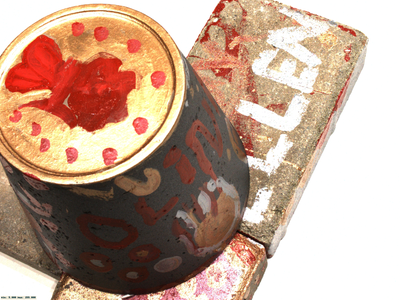
\includegraphics[width=0.15\textwidth]{images/qualitatives/00_keyviews/0.png} & 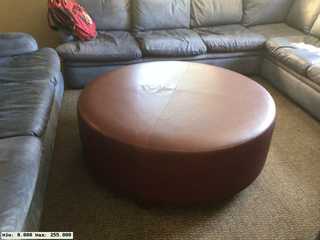
\includegraphics[width=0.15\textwidth]{images/qualitatives/00_keyviews/20.png} & 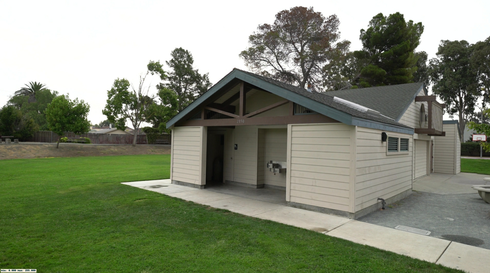
\includegraphics[width=0.15\textwidth, trim={5cm 0 0 0},clip]{images/qualitatives/00_keyviews/6.png} & 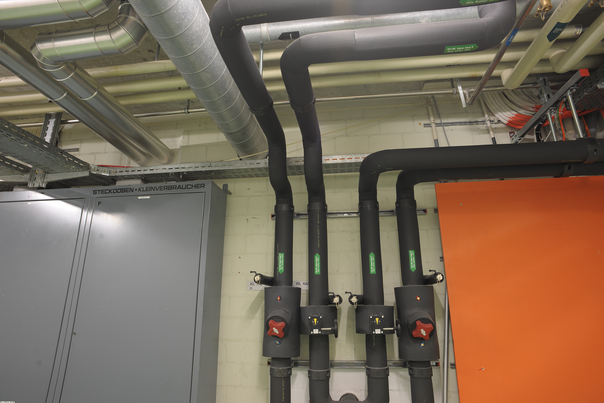
\includegraphics[width=0.15\textwidth]{images/qualitatives/00_keyviews/62.png} & 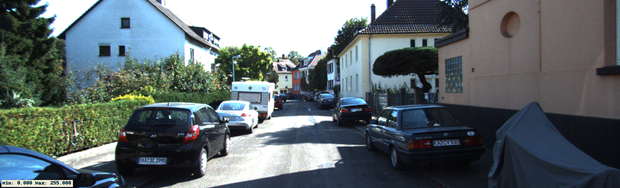
\includegraphics[width=0.15\textwidth, trim={5cm 0 7.5cm 0},clip]{images/qualitatives/00_keyviews/83.png}\\ 
            GT Depth & 
\includegraphics[width=0.15\textwidth]{images/qualitatives/01_depthmaps/0.png} & 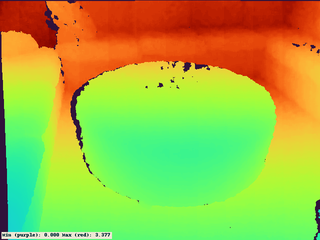
\includegraphics[width=0.15\textwidth]{images/qualitatives/01_depthmaps/20.png} & 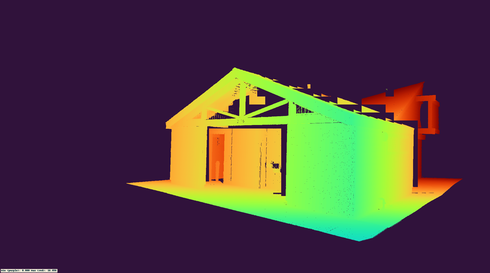
\includegraphics[width=0.15\textwidth, trim={5cm 0 0 0},clip]{images/qualitatives/01_depthmaps/6.png} & 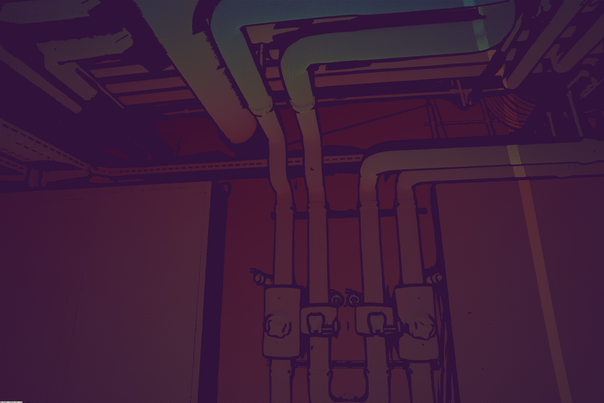
\includegraphics[width=0.15\textwidth]{images/qualitatives/01_depthmaps/62.png} & 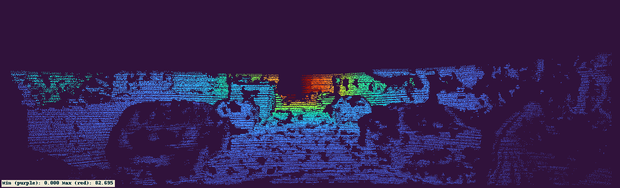
\includegraphics[width=0.15\textwidth, trim={5cm 0 7.5cm 0},clip]{images/qualitatives/01_depthmaps/83.png}\\ 
            {\mvsn} Base\newline $(V=2, D=256)$ \(\star\) & 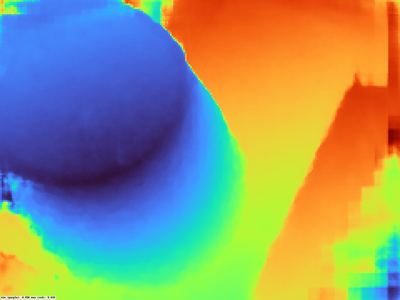
\includegraphics[width=0.15\textwidth]{images/qualitatives/02_mvsn256base/0000000-pred_depth.png} & 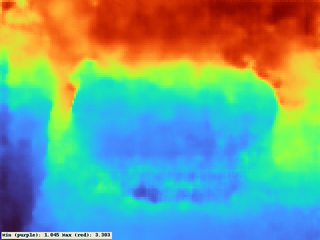
\includegraphics[width=0.15\textwidth]{images/qualitatives/02_mvsn256base/0000020-pred_depth.png} & 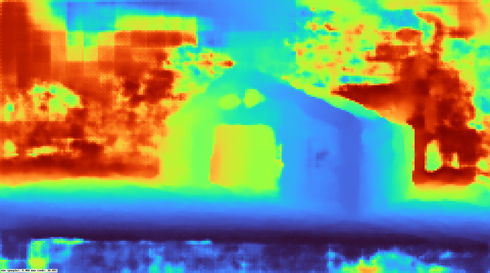
\includegraphics[width=0.15\textwidth, trim={5cm 0 0 0},clip]{images/qualitatives/02_mvsn256base/0000006-pred_depth.png} & 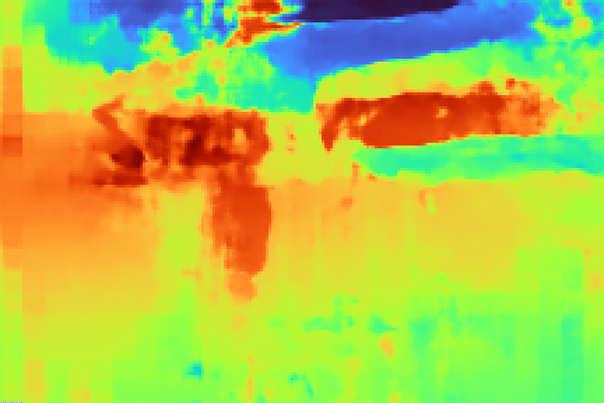
\includegraphics[width=0.15\textwidth]{images/qualitatives/02_mvsn256base/0000062-pred_depth.png} & 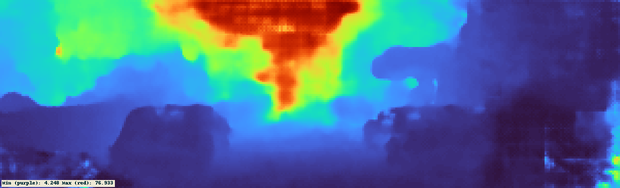
\includegraphics[width=0.15\textwidth, trim={5cm 0 7.5cm 0},clip]{images/qualitatives/02_mvsn256base/0000083-pred_depth.png}\\ 
            {\mvsn} Base\newline $(V=2, D=128)$& 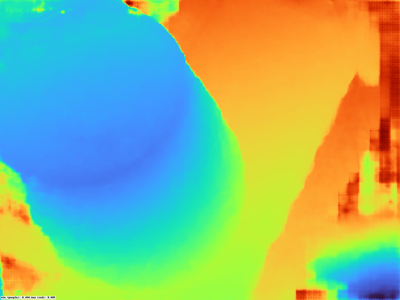
\includegraphics[width=0.15\textwidth]{images/qualitatives/03_mvsn128base/0000000-pred_depth.png} & \includegraphics[width=0.15\textwidth]{images/qualitatives/03_mvsn128base/0000020-pred_depth.png} & 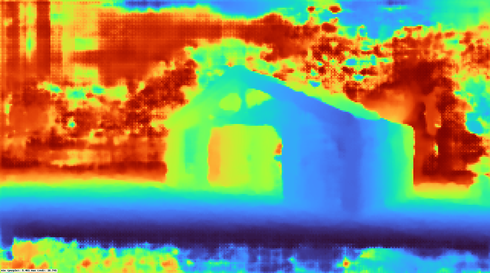
\includegraphics[width=0.15\textwidth, trim={5cm 0 0 0},clip]{images/qualitatives/03_mvsn128base/0000006-pred_depth.png} & 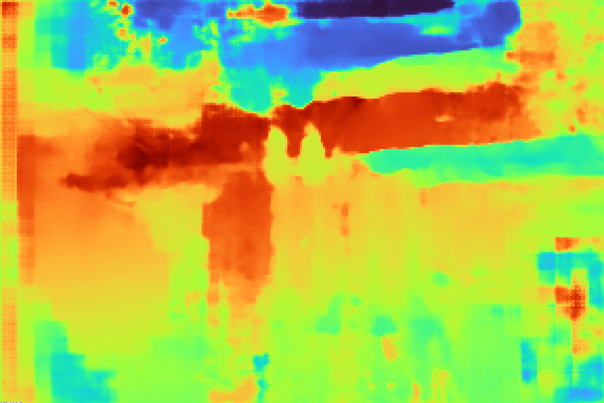
\includegraphics[width=0.15\textwidth]{images/qualitatives/03_mvsn128base/0000062-pred_depth.png} & 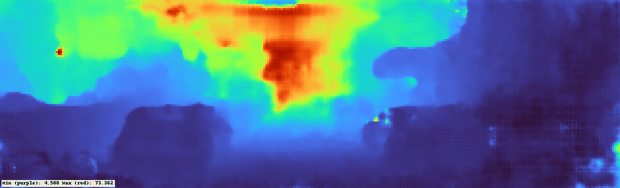
\includegraphics[width=0.15\textwidth, trim={5cm 0 7.5cm 0},clip]{images/qualitatives/03_mvsn128base/0000083-pred_depth.png}\\ 
            {\mvsn} Base\newline $(V=2, D=128)$ \(\star\) & 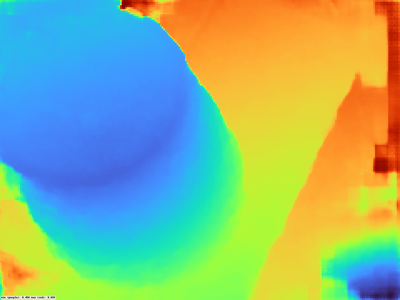
\includegraphics[width=0.15\textwidth]{images/qualitatives/04_mvsn128base_star/0000000-pred_depth.png} & \includegraphics[width=0.15\textwidth]{images/qualitatives/04_mvsn128base_star/0000020-pred_depth.png} & 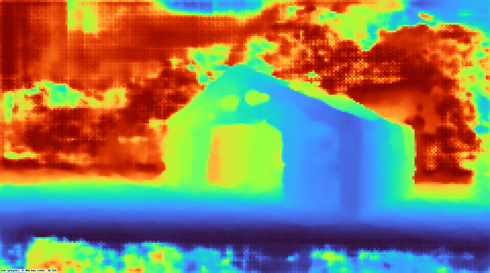
\includegraphics[width=0.15\textwidth, trim={5cm 0 0 0},clip]{images/qualitatives/04_mvsn128base_star/0000006-pred_depth.png} & 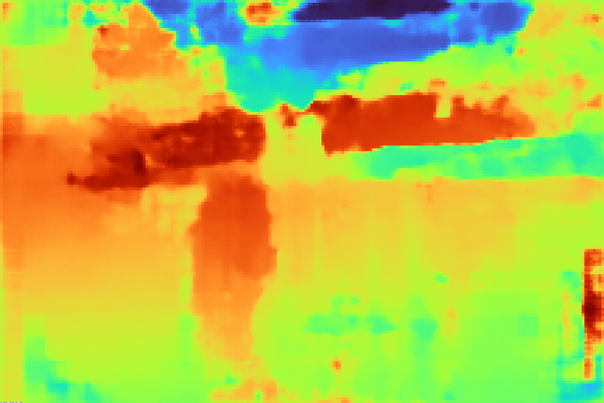
\includegraphics[width=0.15\textwidth]{images/qualitatives/04_mvsn128base_star/0000062-pred_depth.png} & 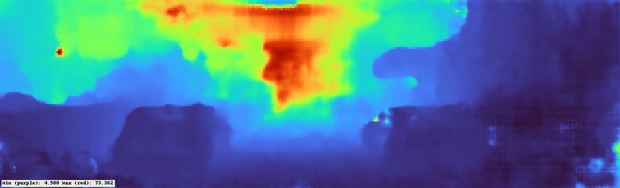
\includegraphics[width=0.15\textwidth, trim={5cm 0 7.5cm 0},clip]{images/qualitatives/04_mvsn128base_star/0000083-pred_depth.png}\\ 
            {\mvsn} Base\newline $(V=2, D=128)$\newline$H=480, W=640$ & 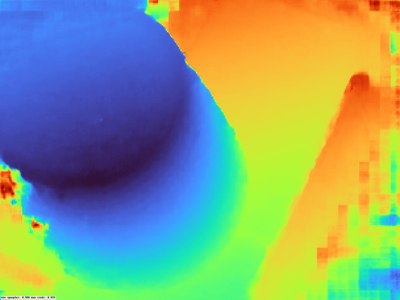
\includegraphics[width=0.15\textwidth]{images/qualitatives/05_mvsn128_sbase/0000000-pred_depth.png} & 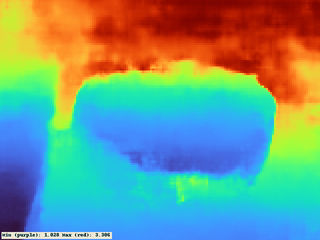
\includegraphics[width=0.15\textwidth]{images/qualitatives/05_mvsn128_sbase/0000020-pred_depth.png} & 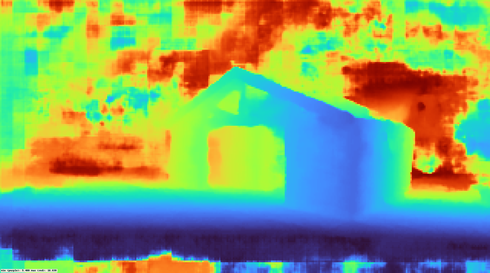
\includegraphics[width=0.15\textwidth, trim={5cm 0 0 0},clip]{images/qualitatives/05_mvsn128_sbase/0000006-pred_depth.png} & 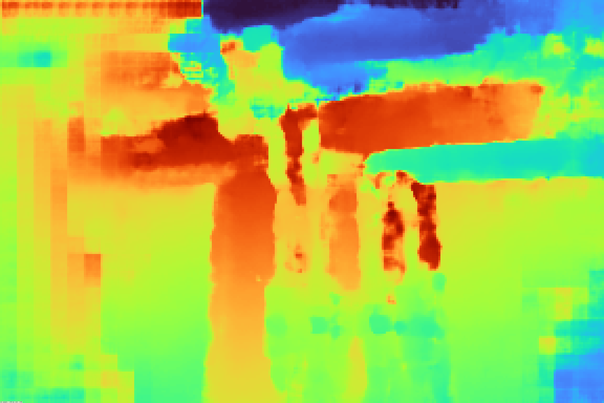
\includegraphics[width=0.15\textwidth]{images/qualitatives/05_mvsn128_sbase/0000062-pred_depth.png} & \includegraphics[width=0.15\textwidth, trim={5cm 0 7.5cm 0},clip]{images/qualitatives/05_mvsn128_sbase/0000083-pred_depth.png}\\ 
            {\mvsn} Base\newline $(V=2, D=128)$\newline$H=480, W=640$ \(\star\) & 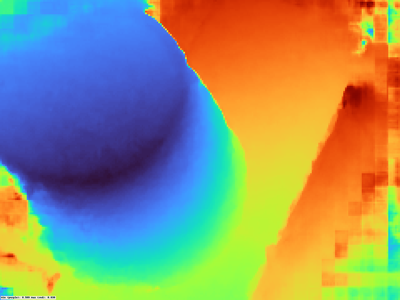
\includegraphics[width=0.15\textwidth]{images/qualitatives/06_mvsn128_sbase_star/0000000-pred_depth.png} & 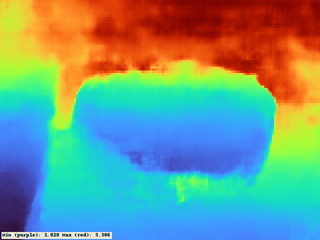
\includegraphics[width=0.15\textwidth]{images/qualitatives/06_mvsn128_sbase_star/0000020-pred_depth.png} & 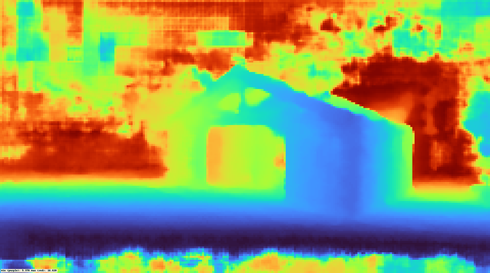
\includegraphics[width=0.15\textwidth, trim={5cm 0 0 0},clip]{images/qualitatives/06_mvsn128_sbase_star/0000006-pred_depth.png} & 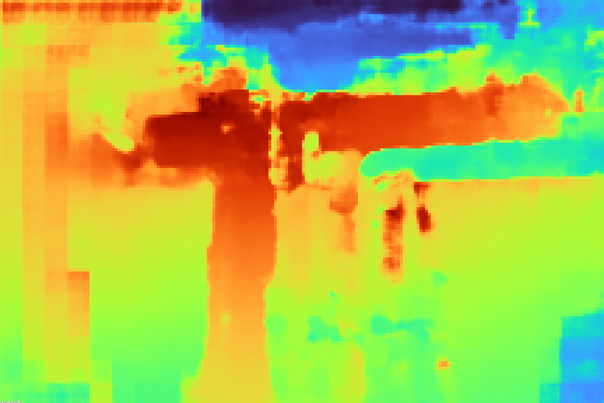
\includegraphics[width=0.15\textwidth]{images/qualitatives/06_mvsn128_sbase_star/0000062-pred_depth.png} & \includegraphics[width=0.15\textwidth, trim={5cm 0 7.5cm 0},clip]{images/qualitatives/06_mvsn128_sbase_star/0000083-pred_depth.png}\\ 
            {\rmvd} Base\newline{\brs}\newline$(V=4 , B=4)$\newline(Baseline from \cite{schroeppel2022benchmark} & 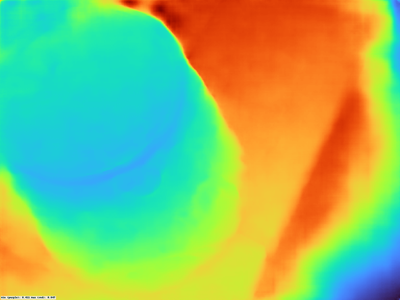
\includegraphics[width=0.15\textwidth]{images/qualitatives/07_rmvdbase/0000000-pred_depth.png} & 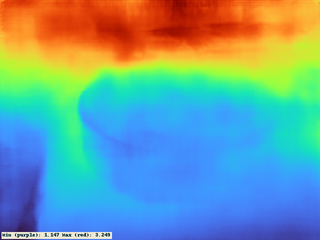
\includegraphics[width=0.15\textwidth]{images/qualitatives/07_rmvdbase/0000020-pred_depth.png} & 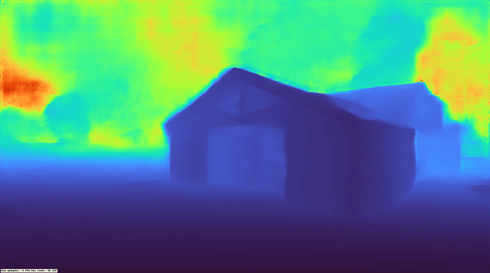
\includegraphics[width=0.15\textwidth, trim={5cm 0 0 0},clip]{images/qualitatives/07_rmvdbase/0000006-pred_depth.png} & 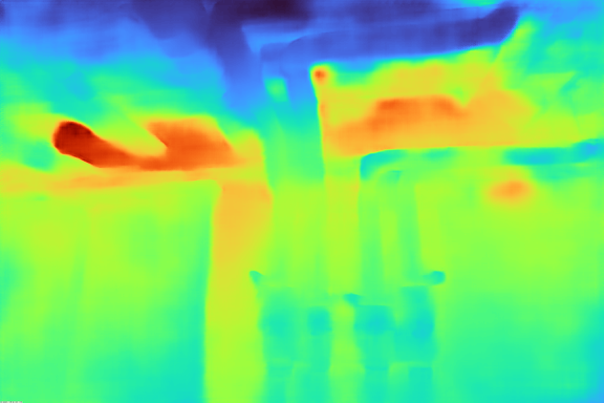
\includegraphics[width=0.15\textwidth]{images/qualitatives/07_rmvdbase/0000062-pred_depth.png} & 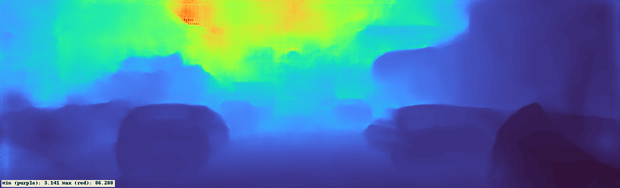
\includegraphics[width=0.15\textwidth, trim={5cm 0 7.5cm 0},clip]{images/qualitatives/07_rmvdbase/0000083-pred_depth.png}\\ 
            {\rmvd} Base\newline{\bms}\newline$(V=2 , B=1)$ & 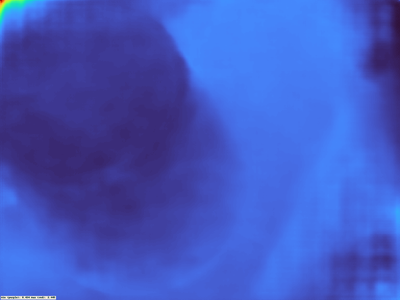
\includegraphics[width=0.15\textwidth]{images/qualitatives/08_rmvd2viewbase/0000000-pred_depth.png} & 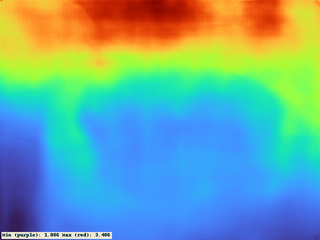
\includegraphics[width=0.15\textwidth]{images/qualitatives/08_rmvd2viewbase/0000020-pred_depth.png} & 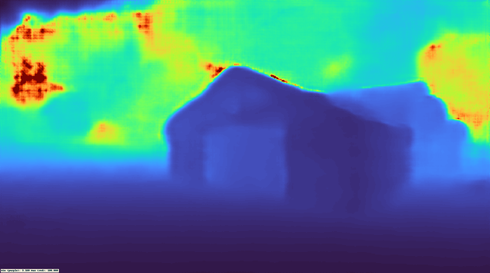
\includegraphics[width=0.15\textwidth, trim={5cm 0 0 0},clip]{images/qualitatives/08_rmvd2viewbase/0000006-pred_depth.png} & \includegraphics[width=0.15\textwidth]{images/qualitatives/08_rmvd2viewbase/0000062-pred_depth.png} & \includegraphics[width=0.15\textwidth, trim={5cm 0 7.5cm 0},clip]{images/qualitatives/08_rmvd2viewbase/0000083-pred_depth.png}\\ 
            {\rmvd} Base\newline{\bms}\newline$(V=2 , B=1)$ \(\star\) & \includegraphics[width=0.15\textwidth]{images/qualitatives/09_rmvd2viewbase_star/0000000-pred_depth.png} & \includegraphics[width=0.15\textwidth]{images/qualitatives/09_rmvd2viewbase_star/0000020-pred_depth.png} & \includegraphics[width=0.15\textwidth, trim={5cm 0 0 0},clip]{images/qualitatives/09_rmvd2viewbase_star/0000006-pred_depth.png} & \includegraphics[width=0.15\textwidth]{images/qualitatives/09_rmvd2viewbase_star/0000062-pred_depth.png} & \includegraphics[width=0.15\textwidth, trim={5cm 0 7.5cm 0},clip]{images/qualitatives/09_rmvd2viewbase_star/0000083-pred_depth.png}\\ 
            MVSNet-pl wrapped\newline(Baseline from \cite{Yao2018}) & \includegraphics[width=0.15\textwidth]{images/qualitatives/10_mvsnplbase/0000000-pred_depth.png} & \includegraphics[width=0.15\textwidth]{images/qualitatives/10_mvsnplbase/0000020-pred_depth.png} & \includegraphics[width=0.15\textwidth, trim={5cm 0 0 0},clip]{images/qualitatives/10_mvsnplbase/0000006-pred_depth.png} & \includegraphics[width=0.15\textwidth]{images/qualitatives/10_mvsnplbase/0000062-pred_depth.png} & \includegraphics[width=0.15\textwidth, trim={5cm 0 7.5cm 0},clip]{images/qualitatives/10_mvsnplbase/0000083-pred_depth.png}\\ 
            MVSNet-pl wrapped \(\star\) & \includegraphics[width=0.15\textwidth]{images/qualitatives/11_mvsnplbase_star/0000000-pred_depth.png} & \includegraphics[width=0.15\textwidth]{images/qualitatives/11_mvsnplbase_star/0000020-pred_depth.png} & \includegraphics[width=0.15\textwidth, trim={5cm 0 0 0},clip]{images/qualitatives/11_mvsnplbase_star/0000006-pred_depth.png} & \includegraphics[width=0.15\textwidth]{images/qualitatives/11_mvsnplbase_star/0000062-pred_depth.png} & \includegraphics[width=0.15\textwidth, trim={5cm 0 7.5cm 0},clip]{images/qualitatives/11_mvsnplbase_star/0000083-pred_depth.png}\\ 
            Vis-MVSNet wrapped\newline(Baseline from \cite{Zhang2020}) & \includegraphics[width=0.15\textwidth]{images/qualitatives/12_vismvsnbase/0000000-pred_depth.png} & \includegraphics[width=0.15\textwidth]{images/qualitatives/12_vismvsnbase/0000020-pred_depth.png} & \includegraphics[width=0.15\textwidth, trim={5cm 0 0 0},clip]{images/qualitatives/12_vismvsnbase/0000006-pred_depth.png} & \includegraphics[width=0.15\textwidth]{images/qualitatives/12_vismvsnbase/0000062-pred_depth.png} & \includegraphics[width=0.15\textwidth, trim={5cm 0 7.5cm 0},clip]{images/qualitatives/12_vismvsnbase/0000083-pred_depth.png}\\ 
            {\mvsn} with\newline DispNet FE\newline$(V=2, D=128)$ & \includegraphics[width=0.15\textwidth]{images/qualitatives/13_mvsn_dispfe/0000000-pred_depth.png} & \includegraphics[width=0.15\textwidth]{images/qualitatives/13_mvsn_dispfe/0000020-pred_depth.png} & \includegraphics[width=0.15\textwidth, trim={5cm 0 0 0},clip]{images/qualitatives/13_mvsn_dispfe/0000006-pred_depth.png} & \includegraphics[width=0.15\textwidth]{images/qualitatives/13_mvsn_dispfe/0000062-pred_depth.png} & \includegraphics[width=0.15\textwidth, trim={5cm 0 7.5cm 0},clip]{images/qualitatives/13_mvsn_dispfe/0000083-pred_depth.png}\\ 
            {\mvsn} with\newline FPN FE\newline$(V=2, D=128)$ & \includegraphics[width=0.15\textwidth]{images/qualitatives/14_mvsn_fpnfe/0000000-pred_depth.png} & \includegraphics[width=0.15\textwidth]{images/qualitatives/14_mvsn_fpnfe/0000020-pred_depth.png} & \includegraphics[width=0.15\textwidth, trim={5cm 0 0 0},clip]{images/qualitatives/14_mvsn_fpnfe/0000006-pred_depth.png} & \includegraphics[width=0.15\textwidth]{images/qualitatives/14_mvsn_fpnfe/0000062-pred_depth.png} & \includegraphics[width=0.15\textwidth, trim={5cm 0 7.5cm 0},clip]{images/qualitatives/14_mvsn_fpnfe/0000083-pred_depth.png}\\ 
            {\mvsn} with\newline UNet FE\newline$(V=2, D=128)$ \(\star\) & \includegraphics[width=0.15\textwidth]{images/qualitatives/15_mvsn_unetfe/0000000-pred_depth.png} & \includegraphics[width=0.15\textwidth]{images/qualitatives/15_mvsn_unetfe/0000020-pred_depth.png} & \includegraphics[width=0.15\textwidth, trim={5cm 0 0 0},clip]{images/qualitatives/15_mvsn_unetfe/0000006-pred_depth.png} & \includegraphics[width=0.15\textwidth]{images/qualitatives/15_mvsn_unetfe/0000062-pred_depth.png} & \includegraphics[width=0.15\textwidth, trim={5cm 0 7.5cm 0},clip]{images/qualitatives/15_mvsn_unetfe/0000083-pred_depth.png}\\ 
            {\mvsn} with\newline DINO ViT FE\newline\((\frac{H}{2}, \frac{W}{2})\)\newline $(H=480, W=640)$ \(\star\) & \includegraphics[width=0.15\textwidth]{images/qualitatives/16_mvsn_dinohalffe/0000000-pred_depth.png} & \includegraphics[width=0.15\textwidth]{images/qualitatives/16_mvsn_dinohalffe/0000020-pred_depth.png} & \includegraphics[width=0.15\textwidth, trim={5cm 0 0 0},clip]{images/qualitatives/16_mvsn_dinohalffe/0000006-pred_depth.png} & \includegraphics[width=0.15\textwidth]{images/qualitatives/16_mvsn_dinohalffe/0000062-pred_depth.png} & \includegraphics[width=0.15\textwidth, trim={5cm 0 7.5cm 0},clip]{images/qualitatives/16_mvsn_dinohalffe/0000083-pred_depth.png}\\ 
            {\mvsn} with\newline DINO ViT FE\newline\((H,W)\)\newline $(H=480, W=640)$ \(\star\) & \includegraphics[width=0.15\textwidth]{images/qualitatives/17_mvsn_dinofullfe/0000000-pred_depth.png} & \includegraphics[width=0.15\textwidth]{images/qualitatives/17_mvsn_dinofullfe/0000020-pred_depth.png} & \includegraphics[width=0.15\textwidth, trim={5cm 0 0 0},clip]{images/qualitatives/17_mvsn_dinofullfe/0000006-pred_depth.png} & \includegraphics[width=0.15\textwidth]{images/qualitatives/17_mvsn_dinofullfe/0000062-pred_depth.png} & \includegraphics[width=0.15\textwidth, trim={5cm 0 7.5cm 0},clip]{images/qualitatives/17_mvsn_dinofullfe/0000083-pred_depth.png}\\ 
            {\rmvd} train on\newline{\brs}\newline{\mvsn} FE\newline($V=4 , B=4$) & \includegraphics[width=0.15\textwidth]{images/qualitatives/18_rmvd_mvsnfe4view/0000000-pred_depth.png} & \includegraphics[width=0.15\textwidth]{images/qualitatives/18_rmvd_mvsnfe4view/0000020-pred_depth.png} & \includegraphics[width=0.15\textwidth, trim={5cm 0 0 0},clip]{images/qualitatives/18_rmvd_mvsnfe4view/0000006-pred_depth.png} & \includegraphics[width=0.15\textwidth]{images/qualitatives/18_rmvd_mvsnfe4view/0000062-pred_depth.png} & \includegraphics[width=0.15\textwidth, trim={5cm 0 7.5cm 0},clip]{images/qualitatives/18_rmvd_mvsnfe4view/0000083-pred_depth.png}\\ 
            {\rmvd} train on\newline{\bms}\newline{\mvsn} FE\newline($V=2 , B=1$) & \includegraphics[width=0.15\textwidth]{images/qualitatives/19_rmvd_mvsnfe2view/0000000-pred_depth.png} & \includegraphics[width=0.15\textwidth]{images/qualitatives/19_rmvd_mvsnfe2view/0000020-pred_depth.png} & \includegraphics[width=0.15\textwidth, trim={5cm 0 0 0},clip]{images/qualitatives/19_rmvd_mvsnfe2view/0000006-pred_depth.png} & \includegraphics[width=0.15\textwidth]{images/qualitatives/19_rmvd_mvsnfe2view/0000062-pred_depth.png} & \includegraphics[width=0.15\textwidth, trim={5cm 0 7.5cm 0},clip]{images/qualitatives/19_rmvd_mvsnfe2view/0000083-pred_depth.png}\\ 
            {\mvsn} with\newline{\gwc}\newline\((G=4)\) & \includegraphics[width=0.15\textwidth]{images/qualitatives/20_mvsn_gwc4_corr/0000000-pred_depth.png} & \includegraphics[width=0.15\textwidth]{images/qualitatives/20_mvsn_gwc4_corr/0000020-pred_depth.png} & \includegraphics[width=0.15\textwidth, trim={5cm 0 0 0},clip]{images/qualitatives/20_mvsn_gwc4_corr/0000006-pred_depth.png} & \includegraphics[width=0.15\textwidth]{images/qualitatives/20_mvsn_gwc4_corr/0000062-pred_depth.png} & \includegraphics[width=0.15\textwidth, trim={5cm 0 7.5cm 0},clip]{images/qualitatives/20_mvsn_gwc4_corr/0000083-pred_depth.png}\\ 
            {\mvsn} with\newline{\gwc}\newline\((G=4)\)\newline and Warp Only & \includegraphics[width=0.15\textwidth]{images/qualitatives/21_mvsn_multicorr/0000000-pred_depth.png} & \includegraphics[width=0.15\textwidth]{images/qualitatives/21_mvsn_multicorr/0000020-pred_depth.png} & \includegraphics[width=0.15\textwidth, trim={5cm 0 0 0},clip]{images/qualitatives/21_mvsn_multicorr/0000006-pred_depth.png} & \includegraphics[width=0.15\textwidth]{images/qualitatives/21_mvsn_multicorr/0000062-pred_depth.png} & \includegraphics[width=0.15\textwidth, trim={5cm 0 7.5cm 0},clip]{images/qualitatives/21_mvsn_multicorr/0000083-pred_depth.png}\\ 
            {\rmvd} with\newline{\gwc}\newline\((G=4)\)\newline(600k iterations) & \includegraphics[width=0.15\textwidth]{images/qualitatives/22_rmvd_gwc4_600k/0000000-pred_depth.png} & \includegraphics[width=0.15\textwidth]{images/qualitatives/22_rmvd_gwc4_600k/0000020-pred_depth.png} & \includegraphics[width=0.15\textwidth, trim={5cm 0 0 0},clip]{images/qualitatives/22_rmvd_gwc4_600k/0000006-pred_depth.png} & \includegraphics[width=0.15\textwidth]{images/qualitatives/22_rmvd_gwc4_600k/0000062-pred_depth.png} & \includegraphics[width=0.15\textwidth, trim={5cm 0 7.5cm 0},clip]{images/qualitatives/22_rmvd_gwc4_600k/0000083-pred_depth.png}\\ 
            {\rmvd} with\newline{\gwc}\newline\((G=4)\)\newline(1000k iterations) & \includegraphics[width=0.15\textwidth]{images/qualitatives/23_rmvd_gwc4_1000k/0000000-pred_depth.png} & \includegraphics[width=0.15\textwidth]{images/qualitatives/23_rmvd_gwc4_1000k/0000020-pred_depth.png} & \includegraphics[width=0.15\textwidth, trim={5cm 0 0 0},clip]{images/qualitatives/23_rmvd_gwc4_1000k/0000006-pred_depth.png} & \includegraphics[width=0.15\textwidth]{images/qualitatives/23_rmvd_gwc4_1000k/0000062-pred_depth.png} & \includegraphics[width=0.15\textwidth, trim={5cm 0 7.5cm 0},clip]{images/qualitatives/23_rmvd_gwc4_1000k/0000083-pred_depth.png}\\ 
            {\rmvd} with\newline{\gwc}\newline\((G=4)\) and \newline Full Correlation & \includegraphics[width=0.15\textwidth]{images/qualitatives/24_rmvd_multicorr/0000000-pred_depth.png} & \includegraphics[width=0.15\textwidth]{images/qualitatives/24_rmvd_multicorr/0000020-pred_depth.png} & \includegraphics[width=0.15\textwidth, trim={5cm 0 0 0},clip]{images/qualitatives/24_rmvd_multicorr/0000006-pred_depth.png} & \includegraphics[width=0.15\textwidth]{images/qualitatives/24_rmvd_multicorr/0000062-pred_depth.png} & \includegraphics[width=0.15\textwidth, trim={5cm 0 7.5cm 0},clip]{images/qualitatives/24_rmvd_multicorr/0000083-pred_depth.png}\\ 
            {\mvsn} with\newline Learned Fusion & \includegraphics[width=0.15\textwidth]{images/qualitatives/25_mvsn_learnedfuse/0000000-pred_depth.png} & \includegraphics[width=0.15\textwidth]{images/qualitatives/25_mvsn_learnedfuse/0000020-pred_depth.png} & \includegraphics[width=0.15\textwidth, trim={5cm 0 0 0},clip]{images/qualitatives/25_mvsn_learnedfuse/0000006-pred_depth.png} & \includegraphics[width=0.15\textwidth]{images/qualitatives/25_mvsn_learnedfuse/0000062-pred_depth.png} & \includegraphics[width=0.15\textwidth, trim={5cm 0 7.5cm 0},clip]{images/qualitatives/25_mvsn_learnedfuse/0000083-pred_depth.png}\\ 
            {\mvsn} with\newline Average Fusion & \includegraphics[width=0.15\textwidth]{images/qualitatives/26_mvsn_avgfuse/0000000-pred_depth.png} & \includegraphics[width=0.15\textwidth]{images/qualitatives/26_mvsn_avgfuse/0000020-pred_depth.png} & \includegraphics[width=0.15\textwidth, trim={5cm 0 0 0},clip]{images/qualitatives/26_mvsn_avgfuse/0000006-pred_depth.png} & \includegraphics[width=0.15\textwidth]{images/qualitatives/26_mvsn_avgfuse/0000062-pred_depth.png} & \includegraphics[width=0.15\textwidth, trim={5cm 0 7.5cm 0},clip]{images/qualitatives/26_mvsn_avgfuse/0000083-pred_depth.png}\\ 
            {\rmvd} train on\newline{\brs}\newline with Average Fusion & \includegraphics[width=0.15\textwidth]{images/qualitatives/27_rmvd_avgfuse/0000000-pred_depth.png} & \includegraphics[width=0.15\textwidth]{images/qualitatives/27_rmvd_avgfuse/0000020-pred_depth.png} & \includegraphics[width=0.15\textwidth, trim={5cm 0 0 0},clip]{images/qualitatives/27_rmvd_avgfuse/0000006-pred_depth.png} & \includegraphics[width=0.15\textwidth]{images/qualitatives/27_rmvd_avgfuse/0000062-pred_depth.png} & \includegraphics[width=0.15\textwidth, trim={5cm 0 7.5cm 0},clip]{images/qualitatives/27_rmvd_avgfuse/0000083-pred_depth.png}\\ 
            {\mvsn} with\newline 2D DispNet Decoder & \includegraphics[width=0.15\textwidth]{images/qualitatives/28_mvsn_dispdec_cvr/0000000-pred_depth.png} & \includegraphics[width=0.15\textwidth]{images/qualitatives/28_mvsn_dispdec_cvr/0000020-pred_depth.png} & \includegraphics[width=0.15\textwidth, trim={5cm 0 0 0},clip]{images/qualitatives/28_mvsn_dispdec_cvr/0000006-pred_depth.png} & \includegraphics[width=0.15\textwidth]{images/qualitatives/28_mvsn_dispdec_cvr/0000062-pred_depth.png} & \includegraphics[width=0.15\textwidth, trim={5cm 0 7.5cm 0},clip]{images/qualitatives/28_mvsn_dispdec_cvr/0000083-pred_depth.png}\\ 
            {\mvsn} with\newline Stacked Hourglass\newline Cost Vol Reg & \includegraphics[width=0.15\textwidth]{images/qualitatives/29_mvsn_stacked_cvr/0000000-pred_depth.png} & \includegraphics[width=0.15\textwidth]{images/qualitatives/29_mvsn_stacked_cvr/0000020-pred_depth.png} & \includegraphics[width=0.15\textwidth, trim={5cm 0 0 0},clip]{images/qualitatives/29_mvsn_stacked_cvr/0000006-pred_depth.png} & \includegraphics[width=0.15\textwidth]{images/qualitatives/29_mvsn_stacked_cvr/0000062-pred_depth.png} & \includegraphics[width=0.15\textwidth, trim={5cm 0 7.5cm 0},clip]{images/qualitatives/29_mvsn_stacked_cvr/0000083-pred_depth.png}\\ 
            {\mvsn}\newline Coarse-to-Fine with\newline FPN FE& \includegraphics[width=0.15\textwidth]{images/qualitatives/30_mvsn_c2f_fpn/0000000-pred_depth.png} & \includegraphics[width=0.15\textwidth]{images/qualitatives/30_mvsn_c2f_fpn/0000020-pred_depth.png} & \includegraphics[width=0.15\textwidth, trim={5cm 0 0 0},clip]{images/qualitatives/30_mvsn_c2f_fpn/0000006-pred_depth.png} & \includegraphics[width=0.15\textwidth]{images/qualitatives/30_mvsn_c2f_fpn/0000062-pred_depth.png} & \includegraphics[width=0.15\textwidth, trim={5cm 0 7.5cm 0},clip]{images/qualitatives/30_mvsn_c2f_fpn/0000083-pred_depth.png}\\ 
            {\mvsn}\newline Coarse-to-Fine with\newline UNet FE& \includegraphics[width=0.15\textwidth]{images/qualitatives/31_mvsn_c2f_unet/0000000-pred_depth.png} & \includegraphics[width=0.15\textwidth]{images/qualitatives/31_mvsn_c2f_unet/0000020-pred_depth.png} & \includegraphics[width=0.15\textwidth, trim={5cm 0 0 0},clip]{images/qualitatives/31_mvsn_c2f_unet/0000006-pred_depth.png} & \includegraphics[width=0.15\textwidth]{images/qualitatives/31_mvsn_c2f_unet/0000062-pred_depth.png} & \includegraphics[width=0.15\textwidth, trim={5cm 0 7.5cm 0},clip]{images/qualitatives/31_mvsn_c2f_unet/0000083-pred_depth.png}\\ 
            {\mvsn} train\newline on {\dtu}\newline\((V=2, D=128)\) & \includegraphics[width=0.15\textwidth]{images/qualitatives/32_mvsn128_dtu_dat/0000000-pred_depth.png} & \includegraphics[width=0.15\textwidth]{images/qualitatives/32_mvsn128_dtu_dat/0000020-pred_depth.png} & \includegraphics[width=0.15\textwidth, trim={5cm 0 0 0},clip]{images/qualitatives/32_mvsn128_dtu_dat/0000006-pred_depth.png} & \includegraphics[width=0.15\textwidth]{images/qualitatives/32_mvsn128_dtu_dat/0000062-pred_depth.png} & \includegraphics[width=0.15\textwidth, trim={5cm 0 7.5cm 0},clip]{images/qualitatives/32_mvsn128_dtu_dat/0000083-pred_depth.png}\\ 
            {\rmvd} train\newline on {\dtu}\newline\((V=2, B=1)\) & \includegraphics[width=0.15\textwidth]{images/qualitatives/33_rmvd_dtu_dat/0000000-pred_depth.png} & \includegraphics[width=0.15\textwidth]{images/qualitatives/33_rmvd_dtu_dat/0000020-pred_depth.png} & \includegraphics[width=0.15\textwidth, trim={5cm 0 0 0},clip]{images/qualitatives/33_rmvd_dtu_dat/0000006-pred_depth.png} & \includegraphics[width=0.15\textwidth]{images/qualitatives/33_rmvd_dtu_dat/0000062-pred_depth.png} & \includegraphics[width=0.15\textwidth, trim={5cm 0 7.5cm 0},clip]{images/qualitatives/33_rmvd_dtu_dat/0000083-pred_depth.png}\\ 
            {\mvsn} with\newline Scale Augmentation & \includegraphics[width=0.15\textwidth]{images/qualitatives/34_mvsn_scale_dat/0000000-pred_depth.png} & \includegraphics[width=0.15\textwidth]{images/qualitatives/34_mvsn_scale_dat/0000020-pred_depth.png} & \includegraphics[width=0.15\textwidth, trim={5cm 0 0 0},clip]{images/qualitatives/34_mvsn_scale_dat/0000006-pred_depth.png} & \includegraphics[width=0.15\textwidth]{images/qualitatives/34_mvsn_scale_dat/0000062-pred_depth.png} & \includegraphics[width=0.15\textwidth, trim={5cm 0 7.5cm 0},clip]{images/qualitatives/34_mvsn_scale_dat/0000083-pred_depth.png}\\ 
            {\rmvd} train on\newline{\brs}\newline without\newline Scale Augmentation & \includegraphics[width=0.15\textwidth]{images/qualitatives/35_rmvd_noscale_dat/0000000-pred_depth.png} & \includegraphics[width=0.15\textwidth]{images/qualitatives/35_rmvd_noscale_dat/0000020-pred_depth.png} & \includegraphics[width=0.15\textwidth, trim={5cm 0 0 0},clip]{images/qualitatives/35_rmvd_noscale_dat/0000006-pred_depth.png} & \includegraphics[width=0.15\textwidth]{images/qualitatives/35_rmvd_noscale_dat/0000062-pred_depth.png} & \includegraphics[width=0.15\textwidth, trim={5cm 0 7.5cm 0},clip]{images/qualitatives/35_rmvd_noscale_dat/0000083-pred_depth.png}\\ 
            {\mvsn} with\newline \((V=4)\)\newline Best Matching Views & \includegraphics[width=0.15\textwidth]{images/qualitatives/36_mvsn_4view_dat/0000000-pred_depth.png} & \includegraphics[width=0.15\textwidth]{images/qualitatives/36_mvsn_4view_dat/0000020-pred_depth.png} & \includegraphics[width=0.15\textwidth, trim={5cm 0 0 0},clip]{images/qualitatives/36_mvsn_4view_dat/0000006-pred_depth.png} & \includegraphics[width=0.15\textwidth]{images/qualitatives/36_mvsn_4view_dat/0000062-pred_depth.png} & \includegraphics[width=0.15\textwidth, trim={5cm 0 7.5cm 0},clip]{images/qualitatives/36_mvsn_4view_dat/0000083-pred_depth.png}\\ 
            {\mvsn} with\newline \((V=2)\)\newline All Combinations - \newline Random Selection & \includegraphics[width=0.15\textwidth]{images/qualitatives/37_mvsn_allcomb_dat/0000000-pred_depth.png} & \includegraphics[width=0.15\textwidth]{images/qualitatives/37_mvsn_allcomb_dat/0000020-pred_depth.png} & \includegraphics[width=0.15\textwidth, trim={5cm 0 0 0},clip]{images/qualitatives/37_mvsn_allcomb_dat/0000006-pred_depth.png} & \includegraphics[width=0.15\textwidth]{images/qualitatives/37_mvsn_allcomb_dat/0000062-pred_depth.png} & \includegraphics[width=0.15\textwidth, trim={5cm 0 7.5cm 0},clip]{images/qualitatives/37_mvsn_allcomb_dat/0000083-pred_depth.png}\\ 
            {\rmvd} with\newline \((V=4)\)\newline Best Matching Views & \includegraphics[width=0.15\textwidth]{images/qualitatives/38_rmvd_best4_dat/0000000-pred_depth.png} & \includegraphics[width=0.15\textwidth]{images/qualitatives/38_rmvd_best4_dat/0000020-pred_depth.png} & \includegraphics[width=0.15\textwidth, trim={5cm 0 0 0},clip]{images/qualitatives/38_rmvd_best4_dat/0000006-pred_depth.png} & \includegraphics[width=0.15\textwidth]{images/qualitatives/38_rmvd_best4_dat/0000062-pred_depth.png} & \includegraphics[width=0.15\textwidth, trim={5cm 0 7.5cm 0},clip]{images/qualitatives/38_rmvd_best4_dat/0000083-pred_depth.png}\\ 
            {\mvsn} with\newline{\gwc}\newline\((G=32)\) & \includegraphics[width=0.15\textwidth]{images/qualitatives/39_mvsn_gwc32_hyp/0000000-pred_depth.png} & \includegraphics[width=0.15\textwidth]{images/qualitatives/39_mvsn_gwc32_hyp/0000020-pred_depth.png} & \includegraphics[width=0.15\textwidth, trim={5cm 0 0 0},clip]{images/qualitatives/39_mvsn_gwc32_hyp/0000006-pred_depth.png} & \includegraphics[width=0.15\textwidth]{images/qualitatives/39_mvsn_gwc32_hyp/0000062-pred_depth.png} & \includegraphics[width=0.15\textwidth, trim={5cm 0 7.5cm 0},clip]{images/qualitatives/39_mvsn_gwc32_hyp/0000083-pred_depth.png}\\ 
            {\mvsn} with \newline Feature Normalization & \includegraphics[width=0.15\textwidth]{images/qualitatives/40_mvsn_128_normt_hyp/0000000-pred_depth.png} & \includegraphics[width=0.15\textwidth]{images/qualitatives/40_mvsn_128_normt_hyp/0000020-pred_depth.png} & \includegraphics[width=0.15\textwidth, trim={5cm 0 0 0},clip]{images/qualitatives/40_mvsn_128_normt_hyp/0000006-pred_depth.png} & \includegraphics[width=0.15\textwidth]{images/qualitatives/40_mvsn_128_normt_hyp/0000062-pred_depth.png} & \includegraphics[width=0.15\textwidth, trim={5cm 0 7.5cm 0},clip]{images/qualitatives/40_mvsn_128_normt_hyp/0000083-pred_depth.png}\\ 
            {\mvsn} with\newline{\gwc}\newline\((G=4)\) and \newline Feature Normalization & \includegraphics[width=0.15\textwidth]{images/qualitatives/41_mvsn_gwc4_normt_hyp/0000000-pred_depth.png} & \includegraphics[width=0.15\textwidth]{images/qualitatives/41_mvsn_gwc4_normt_hyp/0000020-pred_depth.png} & \includegraphics[width=0.15\textwidth, trim={5cm 0 0 0},clip]{images/qualitatives/41_mvsn_gwc4_normt_hyp/0000006-pred_depth.png} & \includegraphics[width=0.15\textwidth]{images/qualitatives/41_mvsn_gwc4_normt_hyp/0000062-pred_depth.png} & \includegraphics[width=0.15\textwidth, trim={5cm 0 7.5cm 0},clip]{images/qualitatives/41_mvsn_gwc4_normt_hyp/0000083-pred_depth.png}\\ 
            {\rmvd} Base\newline \textbf{without} \newline Feature Normalization & \includegraphics[width=0.15\textwidth]{images/qualitatives/42_rmvd_normf_hyp/0000000-pred_depth.png} & \includegraphics[width=0.15\textwidth]{images/qualitatives/42_rmvd_normf_hyp/0000020-pred_depth.png} & \includegraphics[width=0.15\textwidth, trim={5cm 0 0 0},clip]{images/qualitatives/42_rmvd_normf_hyp/0000006-pred_depth.png} & \includegraphics[width=0.15\textwidth]{images/qualitatives/42_rmvd_normf_hyp/0000062-pred_depth.png} & \includegraphics[width=0.15\textwidth, trim={5cm 0 7.5cm 0},clip]{images/qualitatives/42_rmvd_normf_hyp/0000083-pred_depth.png}\\ 

            

        \caption[Qualitative Analysis: Depth Predictions]{\textbf{Qualitative Analysis: Depth Predictions} These depth maps correspond to the quantitative results in the \hyperref[chap:experiments]{Experiments} chapter. We have maintained the same order as that of the experiments to facilitate easier comparison. The pixels shaded in red are farther away compared to the nearby pixels, which are shaded in blue. }
        \label{tab:qual_depth}
    \end{longtable}
\section*{Qualitatives: Uncertainty}

\setlength{\tabcolsep}{0.5pt}
        \begin{longtable}{>{\tiny}M{25mm}M{26mm}M{26mm}M{26mm}M{26mm}M{26mm}}
           
             & {\dtu} & {\scannet} & {\tanksandtemplesshort} & {\ethd} & {\kitti} \\

            Keyviews & \includegraphics[width=0.15\textwidth]{images/qualitatives/00_keyviews/0.png} & \includegraphics[width=0.15\textwidth]{images/qualitatives/00_keyviews/20.png} & \includegraphics[width=0.15\textwidth, trim={5cm 0 0 0},clip]{images/qualitatives/00_keyviews/6.png} & \includegraphics[width=0.15\textwidth]{images/qualitatives/00_keyviews/62.png} & \includegraphics[width=0.15\textwidth, trim={5cm 0 7.5cm 0},clip]{images/qualitatives/00_keyviews/83.png}\\ 
            GT Depth & \includegraphics[width=0.15\textwidth]{images/qualitatives/01_depthmaps/0.png} & \includegraphics[width=0.15\textwidth]{images/qualitatives/01_depthmaps/20.png} & \includegraphics[width=0.15\textwidth, trim={5cm 0 0 0},clip]{images/qualitatives/01_depthmaps/6.png} & \includegraphics[width=0.15\textwidth]{images/qualitatives/01_depthmaps/62.png} & \includegraphics[width=0.15\textwidth, trim={5cm 0 7.5cm 0},clip]{images/qualitatives/01_depthmaps/83.png}\\ 
            {\mvsn} Base\newline $(V=2, D=256)$ \(\star\) & \includegraphics[width=0.15\textwidth]{images/qualitatives/02_mvsn256base/0000000-pred_depth_uncertainty.png} & \includegraphics[width=0.15\textwidth]{images/qualitatives/02_mvsn256base/0000020-pred_depth_uncertainty.png} & \includegraphics[width=0.15\textwidth, trim={5cm 0 0 0},clip]{images/qualitatives/02_mvsn256base/0000006-pred_depth_uncertainty.png} & \includegraphics[width=0.15\textwidth]{images/qualitatives/02_mvsn256base/0000062-pred_depth_uncertainty.png} & \includegraphics[width=0.15\textwidth, trim={5cm 0 7.5cm 0},clip]{images/qualitatives/02_mvsn256base/0000083-pred_depth_uncertainty.png}\\ 
            {\mvsn} Base\newline $(V=2, D=128)$& \includegraphics[width=0.15\textwidth]{images/qualitatives/03_mvsn128base/0000000-pred_depth_uncertainty.png} & \includegraphics[width=0.15\textwidth]{images/qualitatives/03_mvsn128base/0000020-pred_depth_uncertainty.png} & \includegraphics[width=0.15\textwidth, trim={5cm 0 0 0},clip]{images/qualitatives/03_mvsn128base/0000006-pred_depth_uncertainty.png} & \includegraphics[width=0.15\textwidth]{images/qualitatives/03_mvsn128base/0000062-pred_depth_uncertainty.png} & \includegraphics[width=0.15\textwidth, trim={5cm 0 7.5cm 0},clip]{images/qualitatives/03_mvsn128base/0000083-pred_depth_uncertainty.png}\\ 
            {\mvsn} Base\newline $(V=2, D=128)$ \(\star\) & \includegraphics[width=0.15\textwidth]{images/qualitatives/04_mvsn128base_star/0000000-pred_depth_uncertainty.png} & \includegraphics[width=0.15\textwidth]{images/qualitatives/04_mvsn128base_star/0000020-pred_depth_uncertainty.png} & \includegraphics[width=0.15\textwidth, trim={5cm 0 0 0},clip]{images/qualitatives/04_mvsn128base_star/0000006-pred_depth_uncertainty.png} & \includegraphics[width=0.15\textwidth]{images/qualitatives/04_mvsn128base_star/0000062-pred_depth_uncertainty.png} & \includegraphics[width=0.15\textwidth, trim={5cm 0 7.5cm 0},clip]{images/qualitatives/04_mvsn128base_star/0000083-pred_depth_uncertainty.png}\\ 
            {\mvsn} Base\newline $(V=2, D=128)$\newline$H=480, W=640$ & \includegraphics[width=0.15\textwidth]{images/qualitatives/05_mvsn128_sbase/0000000-pred_depth_uncertainty.png} & \includegraphics[width=0.15\textwidth]{images/qualitatives/05_mvsn128_sbase/0000020-pred_depth_uncertainty.png} & \includegraphics[width=0.15\textwidth, trim={5cm 0 0 0},clip]{images/qualitatives/05_mvsn128_sbase/0000006-pred_depth_uncertainty.png} & \includegraphics[width=0.15\textwidth]{images/qualitatives/05_mvsn128_sbase/0000062-pred_depth_uncertainty.png} & \includegraphics[width=0.15\textwidth, trim={5cm 0 7.5cm 0},clip]{images/qualitatives/05_mvsn128_sbase/0000083-pred_depth_uncertainty.png}\\ 
            {\mvsn} Base\newline $(V=2, D=128)$\newline$H=480, W=640$ \(\star\) & \includegraphics[width=0.15\textwidth]{images/qualitatives/06_mvsn128_sbase_star/0000000-pred_depth_uncertainty.png} & \includegraphics[width=0.15\textwidth]{images/qualitatives/06_mvsn128_sbase_star/0000020-pred_depth_uncertainty.png} & \includegraphics[width=0.15\textwidth, trim={5cm 0 0 0},clip]{images/qualitatives/06_mvsn128_sbase_star/0000006-pred_depth_uncertainty.png} & \includegraphics[width=0.15\textwidth]{images/qualitatives/06_mvsn128_sbase_star/0000062-pred_depth_uncertainty.png} & \includegraphics[width=0.15\textwidth, trim={5cm 0 7.5cm 0},clip]{images/qualitatives/06_mvsn128_sbase_star/0000083-pred_depth_uncertainty.png}\\ 
            {\rmvd} Base\newline{\brs}\newline$(V=4 , B=4)$\newline(Baseline from \cite{schroeppel2022benchmark} & \includegraphics[width=0.15\textwidth]{images/qualitatives/07_rmvdbase/0000000-pred_depth_uncertainty.png} & \includegraphics[width=0.15\textwidth]{images/qualitatives/07_rmvdbase/0000020-pred_depth_uncertainty.png} & \includegraphics[width=0.15\textwidth, trim={5cm 0 0 0},clip]{images/qualitatives/07_rmvdbase/0000006-pred_depth_uncertainty.png} & \includegraphics[width=0.15\textwidth]{images/qualitatives/07_rmvdbase/0000062-pred_depth_uncertainty.png} & \includegraphics[width=0.15\textwidth, trim={5cm 0 7.5cm 0},clip]{images/qualitatives/07_rmvdbase/0000083-pred_depth_uncertainty.png}\\ 
            {\rmvd} Base\newline{\bms}\newline$(V=2 , B=1)$ & \includegraphics[width=0.15\textwidth]{images/qualitatives/08_rmvd2viewbase/0000000-pred_depth_uncertainty.png} & \includegraphics[width=0.15\textwidth]{images/qualitatives/08_rmvd2viewbase/0000020-pred_depth_uncertainty.png} & \includegraphics[width=0.15\textwidth, trim={5cm 0 0 0},clip]{images/qualitatives/08_rmvd2viewbase/0000006-pred_depth_uncertainty.png} & \includegraphics[width=0.15\textwidth]{images/qualitatives/08_rmvd2viewbase/0000062-pred_depth_uncertainty.png} & \includegraphics[width=0.15\textwidth, trim={5cm 0 7.5cm 0},clip]{images/qualitatives/08_rmvd2viewbase/0000083-pred_depth_uncertainty.png}\\ 
            {\rmvd} Base\newline{\bms}\newline$(V=2 , B=1)$ \(\star\) & \includegraphics[width=0.15\textwidth]{images/qualitatives/09_rmvd2viewbase_star/0000000-pred_depth_uncertainty.png} & \includegraphics[width=0.15\textwidth]{images/qualitatives/09_rmvd2viewbase_star/0000020-pred_depth_uncertainty.png} & \includegraphics[width=0.15\textwidth, trim={5cm 0 0 0},clip]{images/qualitatives/09_rmvd2viewbase_star/0000006-pred_depth_uncertainty.png} & \includegraphics[width=0.15\textwidth]{images/qualitatives/09_rmvd2viewbase_star/0000062-pred_depth_uncertainty.png} & \includegraphics[width=0.15\textwidth, trim={5cm 0 7.5cm 0},clip]{images/qualitatives/09_rmvd2viewbase_star/0000083-pred_depth_uncertainty.png}\\ 
            MVSNet-pl wrapped\newline(Baseline from \cite{Yao2018}) & \includegraphics[width=0.15\textwidth]{images/qualitatives/10_mvsnplbase/0000000-pred_depth_uncertainty.png} & \includegraphics[width=0.15\textwidth]{images/qualitatives/10_mvsnplbase/0000020-pred_depth_uncertainty.png} & \includegraphics[width=0.15\textwidth, trim={5cm 0 0 0},clip]{images/qualitatives/10_mvsnplbase/0000006-pred_depth_uncertainty.png} & \includegraphics[width=0.15\textwidth]{images/qualitatives/10_mvsnplbase/0000062-pred_depth_uncertainty.png} & \includegraphics[width=0.15\textwidth, trim={5cm 0 7.5cm 0},clip]{images/qualitatives/10_mvsnplbase/0000083-pred_depth_uncertainty.png}\\ 
            MVSNet-pl wrapped \(\star\) & \includegraphics[width=0.15\textwidth]{images/qualitatives/11_mvsnplbase_star/0000000-pred_depth_uncertainty.png} & \includegraphics[width=0.15\textwidth]{images/qualitatives/11_mvsnplbase_star/0000020-pred_depth_uncertainty.png} & \includegraphics[width=0.15\textwidth, trim={5cm 0 0 0},clip]{images/qualitatives/11_mvsnplbase_star/0000006-pred_depth_uncertainty.png} & \includegraphics[width=0.15\textwidth]{images/qualitatives/11_mvsnplbase_star/0000062-pred_depth_uncertainty.png} & \includegraphics[width=0.15\textwidth, trim={5cm 0 7.5cm 0},clip]{images/qualitatives/11_mvsnplbase_star/0000083-pred_depth_uncertainty.png}\\ 
            Vis-MVSNet wrapped\newline(Baseline from \cite{Zhang2020}) & \includegraphics[width=0.15\textwidth]{images/qualitatives/12_vismvsnbase/0000000-pred_depth_uncertainty.png} & \includegraphics[width=0.15\textwidth]{images/qualitatives/12_vismvsnbase/0000020-pred_depth_uncertainty.png} & \includegraphics[width=0.15\textwidth, trim={5cm 0 0 0},clip]{images/qualitatives/12_vismvsnbase/0000006-pred_depth_uncertainty.png} & \includegraphics[width=0.15\textwidth]{images/qualitatives/12_vismvsnbase/0000062-pred_depth_uncertainty.png} & \includegraphics[width=0.15\textwidth, trim={5cm 0 7.5cm 0},clip]{images/qualitatives/12_vismvsnbase/0000083-pred_depth_uncertainty.png}\\ 
            {\mvsn} with\newline DispNet FE\newline$(V=2, D=128)$ & \includegraphics[width=0.15\textwidth]{images/qualitatives/13_mvsn_dispfe/0000000-pred_depth_uncertainty.png} & \includegraphics[width=0.15\textwidth]{images/qualitatives/13_mvsn_dispfe/0000020-pred_depth_uncertainty.png} & \includegraphics[width=0.15\textwidth, trim={5cm 0 0 0},clip]{images/qualitatives/13_mvsn_dispfe/0000006-pred_depth_uncertainty.png} & \includegraphics[width=0.15\textwidth]{images/qualitatives/13_mvsn_dispfe/0000062-pred_depth_uncertainty.png} & \includegraphics[width=0.15\textwidth, trim={5cm 0 7.5cm 0},clip]{images/qualitatives/13_mvsn_dispfe/0000083-pred_depth_uncertainty.png}\\ 
            {\mvsn} with\newline FPN FE\newline$(V=2, D=128)$ & \includegraphics[width=0.15\textwidth]{images/qualitatives/14_mvsn_fpnfe/0000000-pred_depth_uncertainty.png} & \includegraphics[width=0.15\textwidth]{images/qualitatives/14_mvsn_fpnfe/0000020-pred_depth_uncertainty.png} & \includegraphics[width=0.15\textwidth, trim={5cm 0 0 0},clip]{images/qualitatives/14_mvsn_fpnfe/0000006-pred_depth_uncertainty.png} & \includegraphics[width=0.15\textwidth]{images/qualitatives/14_mvsn_fpnfe/0000062-pred_depth_uncertainty.png} & \includegraphics[width=0.15\textwidth, trim={5cm 0 7.5cm 0},clip]{images/qualitatives/14_mvsn_fpnfe/0000083-pred_depth_uncertainty.png}\\ 
            {\mvsn} with\newline UNet FE\newline$(V=2, D=128)$ \(\star\) & \includegraphics[width=0.15\textwidth]{images/qualitatives/15_mvsn_unetfe/0000000-pred_depth_uncertainty.png} & \includegraphics[width=0.15\textwidth]{images/qualitatives/15_mvsn_unetfe/0000020-pred_depth_uncertainty.png} & \includegraphics[width=0.15\textwidth, trim={5cm 0 0 0},clip]{images/qualitatives/15_mvsn_unetfe/0000006-pred_depth_uncertainty.png} & \includegraphics[width=0.15\textwidth]{images/qualitatives/15_mvsn_unetfe/0000062-pred_depth_uncertainty.png} & \includegraphics[width=0.15\textwidth, trim={5cm 0 7.5cm 0},clip]{images/qualitatives/15_mvsn_unetfe/0000083-pred_depth_uncertainty.png}\\ 
            {\mvsn} with\newline DINO ViT FE\newline\((\frac{H}{2}, \frac{W}{2})\)\newline $(H=480, W=640)$ \(\star\) & \includegraphics[width=0.15\textwidth]{images/qualitatives/16_mvsn_dinohalffe/0000000-pred_depth_uncertainty.png} & \includegraphics[width=0.15\textwidth]{images/qualitatives/16_mvsn_dinohalffe/0000020-pred_depth_uncertainty.png} & \includegraphics[width=0.15\textwidth, trim={5cm 0 0 0},clip]{images/qualitatives/16_mvsn_dinohalffe/0000006-pred_depth_uncertainty.png} & \includegraphics[width=0.15\textwidth]{images/qualitatives/16_mvsn_dinohalffe/0000062-pred_depth_uncertainty.png} & \includegraphics[width=0.15\textwidth, trim={5cm 0 7.5cm 0},clip]{images/qualitatives/16_mvsn_dinohalffe/0000083-pred_depth_uncertainty.png}\\ 
            {\mvsn} with\newline DINO ViT FE\newline\((H,W)\)\newline $(H=480, W=640)$ \(\star\) & \includegraphics[width=0.15\textwidth]{images/qualitatives/17_mvsn_dinofullfe/0000000-pred_depth_uncertainty.png} & \includegraphics[width=0.15\textwidth]{images/qualitatives/17_mvsn_dinofullfe/0000020-pred_depth_uncertainty.png} & \includegraphics[width=0.15\textwidth, trim={5cm 0 0 0},clip]{images/qualitatives/17_mvsn_dinofullfe/0000006-pred_depth_uncertainty.png} & \includegraphics[width=0.15\textwidth]{images/qualitatives/17_mvsn_dinofullfe/0000062-pred_depth_uncertainty.png} & \includegraphics[width=0.15\textwidth, trim={5cm 0 7.5cm 0},clip]{images/qualitatives/17_mvsn_dinofullfe/0000083-pred_depth_uncertainty.png}\\ 
            {\rmvd} train on\newline{\brs}\newline{\mvsn} FE\newline($V=4 , B=4$) & \includegraphics[width=0.15\textwidth]{images/qualitatives/18_rmvd_mvsnfe4view/0000000-pred_depth_uncertainty.png} & \includegraphics[width=0.15\textwidth]{images/qualitatives/18_rmvd_mvsnfe4view/0000020-pred_depth_uncertainty.png} & \includegraphics[width=0.15\textwidth, trim={5cm 0 0 0},clip]{images/qualitatives/18_rmvd_mvsnfe4view/0000006-pred_depth_uncertainty.png} & \includegraphics[width=0.15\textwidth]{images/qualitatives/18_rmvd_mvsnfe4view/0000062-pred_depth_uncertainty.png} & \includegraphics[width=0.15\textwidth, trim={5cm 0 7.5cm 0},clip]{images/qualitatives/18_rmvd_mvsnfe4view/0000083-pred_depth_uncertainty.png}\\ 
            {\rmvd} train on\newline{\bms}\newline{\mvsn} FE\newline($V=2 , B=1$) & \includegraphics[width=0.15\textwidth]{images/qualitatives/19_rmvd_mvsnfe2view/0000000-pred_depth_uncertainty.png} & \includegraphics[width=0.15\textwidth]{images/qualitatives/19_rmvd_mvsnfe2view/0000020-pred_depth_uncertainty.png} & \includegraphics[width=0.15\textwidth, trim={5cm 0 0 0},clip]{images/qualitatives/19_rmvd_mvsnfe2view/0000006-pred_depth_uncertainty.png} & \includegraphics[width=0.15\textwidth]{images/qualitatives/19_rmvd_mvsnfe2view/0000062-pred_depth_uncertainty.png} & \includegraphics[width=0.15\textwidth, trim={5cm 0 7.5cm 0},clip]{images/qualitatives/19_rmvd_mvsnfe2view/0000083-pred_depth_uncertainty.png}\\ 
            {\mvsn} with\newline{\gwc}\newline\((G=4)\) & \includegraphics[width=0.15\textwidth]{images/qualitatives/20_mvsn_gwc4_corr/0000000-pred_depth_uncertainty.png} & \includegraphics[width=0.15\textwidth]{images/qualitatives/20_mvsn_gwc4_corr/0000020-pred_depth_uncertainty.png} & \includegraphics[width=0.15\textwidth, trim={5cm 0 0 0},clip]{images/qualitatives/20_mvsn_gwc4_corr/0000006-pred_depth_uncertainty.png} & \includegraphics[width=0.15\textwidth]{images/qualitatives/20_mvsn_gwc4_corr/0000062-pred_depth_uncertainty.png} & \includegraphics[width=0.15\textwidth, trim={5cm 0 7.5cm 0},clip]{images/qualitatives/20_mvsn_gwc4_corr/0000083-pred_depth_uncertainty.png}\\ 
            {\mvsn} with\newline{\gwc}\newline\((G=4)\)\newline and Warp Only & \includegraphics[width=0.15\textwidth]{images/qualitatives/21_mvsn_multicorr/0000000-pred_depth_uncertainty.png} & \includegraphics[width=0.15\textwidth]{images/qualitatives/21_mvsn_multicorr/0000020-pred_depth_uncertainty.png} & \includegraphics[width=0.15\textwidth, trim={5cm 0 0 0},clip]{images/qualitatives/21_mvsn_multicorr/0000006-pred_depth_uncertainty.png} & \includegraphics[width=0.15\textwidth]{images/qualitatives/21_mvsn_multicorr/0000062-pred_depth_uncertainty.png} & \includegraphics[width=0.15\textwidth, trim={5cm 0 7.5cm 0},clip]{images/qualitatives/21_mvsn_multicorr/0000083-pred_depth_uncertainty.png}\\ 
            {\rmvd} with\newline{\gwc}\newline\((G=4)\)\newline(600k iterations) & \includegraphics[width=0.15\textwidth]{images/qualitatives/22_rmvd_gwc4_600k/0000000-pred_depth_uncertainty.png} & \includegraphics[width=0.15\textwidth]{images/qualitatives/22_rmvd_gwc4_600k/0000020-pred_depth_uncertainty.png} & \includegraphics[width=0.15\textwidth, trim={5cm 0 0 0},clip]{images/qualitatives/22_rmvd_gwc4_600k/0000006-pred_depth_uncertainty.png} & \includegraphics[width=0.15\textwidth]{images/qualitatives/22_rmvd_gwc4_600k/0000062-pred_depth_uncertainty.png} & \includegraphics[width=0.15\textwidth, trim={5cm 0 7.5cm 0},clip]{images/qualitatives/22_rmvd_gwc4_600k/0000083-pred_depth_uncertainty.png}\\ 
            {\rmvd} with\newline{\gwc}\newline\((G=4)\)\newline(1000k iterations) & \includegraphics[width=0.15\textwidth]{images/qualitatives/23_rmvd_gwc4_1000k/0000000-pred_depth_uncertainty.png} & \includegraphics[width=0.15\textwidth]{images/qualitatives/23_rmvd_gwc4_1000k/0000020-pred_depth_uncertainty.png} & \includegraphics[width=0.15\textwidth, trim={5cm 0 0 0},clip]{images/qualitatives/23_rmvd_gwc4_1000k/0000006-pred_depth_uncertainty.png} & \includegraphics[width=0.15\textwidth]{images/qualitatives/23_rmvd_gwc4_1000k/0000062-pred_depth_uncertainty.png} & \includegraphics[width=0.15\textwidth, trim={5cm 0 7.5cm 0},clip]{images/qualitatives/23_rmvd_gwc4_1000k/0000083-pred_depth_uncertainty.png}\\ 
            {\rmvd} with\newline{\gwc}\newline\((G=4)\) and \newline Full Correlation & \includegraphics[width=0.15\textwidth]{images/qualitatives/24_rmvd_multicorr/0000000-pred_depth_uncertainty.png} & \includegraphics[width=0.15\textwidth]{images/qualitatives/24_rmvd_multicorr/0000020-pred_depth_uncertainty.png} & \includegraphics[width=0.15\textwidth, trim={5cm 0 0 0},clip]{images/qualitatives/24_rmvd_multicorr/0000006-pred_depth_uncertainty.png} & \includegraphics[width=0.15\textwidth]{images/qualitatives/24_rmvd_multicorr/0000062-pred_depth_uncertainty.png} & \includegraphics[width=0.15\textwidth, trim={5cm 0 7.5cm 0},clip]{images/qualitatives/24_rmvd_multicorr/0000083-pred_depth_uncertainty.png}\\ 
            {\mvsn} with\newline Learned Fusion & \includegraphics[width=0.15\textwidth]{images/qualitatives/25_mvsn_learnedfuse/0000000-pred_depth_uncertainty.png} & \includegraphics[width=0.15\textwidth]{images/qualitatives/25_mvsn_learnedfuse/0000020-pred_depth_uncertainty.png} & \includegraphics[width=0.15\textwidth, trim={5cm 0 0 0},clip]{images/qualitatives/25_mvsn_learnedfuse/0000006-pred_depth_uncertainty.png} & \includegraphics[width=0.15\textwidth]{images/qualitatives/25_mvsn_learnedfuse/0000062-pred_depth_uncertainty.png} & \includegraphics[width=0.15\textwidth, trim={5cm 0 7.5cm 0},clip]{images/qualitatives/25_mvsn_learnedfuse/0000083-pred_depth_uncertainty.png}\\ 
            {\mvsn} with\newline Average Fusion & \includegraphics[width=0.15\textwidth]{images/qualitatives/26_mvsn_avgfuse/0000000-pred_depth_uncertainty.png} & \includegraphics[width=0.15\textwidth]{images/qualitatives/26_mvsn_avgfuse/0000020-pred_depth_uncertainty.png} & \includegraphics[width=0.15\textwidth, trim={5cm 0 0 0},clip]{images/qualitatives/26_mvsn_avgfuse/0000006-pred_depth_uncertainty.png} & \includegraphics[width=0.15\textwidth]{images/qualitatives/26_mvsn_avgfuse/0000062-pred_depth_uncertainty.png} & \includegraphics[width=0.15\textwidth, trim={5cm 0 7.5cm 0},clip]{images/qualitatives/26_mvsn_avgfuse/0000083-pred_depth_uncertainty.png}\\ 
            {\rmvd} train on\newline{\brs}\newline with Average Fusion & \includegraphics[width=0.15\textwidth]{images/qualitatives/27_rmvd_avgfuse/0000000-pred_depth_uncertainty.png} & \includegraphics[width=0.15\textwidth]{images/qualitatives/27_rmvd_avgfuse/0000020-pred_depth_uncertainty.png} & \includegraphics[width=0.15\textwidth, trim={5cm 0 0 0},clip]{images/qualitatives/27_rmvd_avgfuse/0000006-pred_depth_uncertainty.png} & \includegraphics[width=0.15\textwidth]{images/qualitatives/27_rmvd_avgfuse/0000062-pred_depth_uncertainty.png} & \includegraphics[width=0.15\textwidth, trim={5cm 0 7.5cm 0},clip]{images/qualitatives/27_rmvd_avgfuse/0000083-pred_depth_uncertainty.png}\\ 
            {\mvsn} with\newline 2D DispNet Decoder & \includegraphics[width=0.15\textwidth]{images/qualitatives/28_mvsn_dispdec_cvr/0000000-pred_depth_uncertainty.png} & \includegraphics[width=0.15\textwidth]{images/qualitatives/28_mvsn_dispdec_cvr/0000020-pred_depth_uncertainty.png} & \includegraphics[width=0.15\textwidth, trim={5cm 0 0 0},clip]{images/qualitatives/28_mvsn_dispdec_cvr/0000006-pred_depth_uncertainty.png} & \includegraphics[width=0.15\textwidth]{images/qualitatives/28_mvsn_dispdec_cvr/0000062-pred_depth_uncertainty.png} & \includegraphics[width=0.15\textwidth, trim={5cm 0 7.5cm 0},clip]{images/qualitatives/28_mvsn_dispdec_cvr/0000083-pred_depth_uncertainty.png}\\ 
            {\mvsn} with\newline Stacked Hourglass\newline Cost Vol Reg & \includegraphics[width=0.15\textwidth]{images/qualitatives/29_mvsn_stacked_cvr/0000000-pred_depth_uncertainty.png} & \includegraphics[width=0.15\textwidth]{images/qualitatives/29_mvsn_stacked_cvr/0000020-pred_depth_uncertainty.png} & \includegraphics[width=0.15\textwidth, trim={5cm 0 0 0},clip]{images/qualitatives/29_mvsn_stacked_cvr/0000006-pred_depth_uncertainty.png} & \includegraphics[width=0.15\textwidth]{images/qualitatives/29_mvsn_stacked_cvr/0000062-pred_depth_uncertainty.png} & \includegraphics[width=0.15\textwidth, trim={5cm 0 7.5cm 0},clip]{images/qualitatives/29_mvsn_stacked_cvr/0000083-pred_depth_uncertainty.png}\\ 
            {\mvsn}\newline Coarse-to-Fine with\newline FPN FE& \includegraphics[width=0.15\textwidth]{images/qualitatives/30_mvsn_c2f_fpn/0000000-pred_depth_uncertainty.png} & \includegraphics[width=0.15\textwidth]{images/qualitatives/30_mvsn_c2f_fpn/0000020-pred_depth_uncertainty.png} & \includegraphics[width=0.15\textwidth, trim={5cm 0 0 0},clip]{images/qualitatives/30_mvsn_c2f_fpn/0000006-pred_depth_uncertainty.png} & \includegraphics[width=0.15\textwidth]{images/qualitatives/30_mvsn_c2f_fpn/0000062-pred_depth_uncertainty.png} & \includegraphics[width=0.15\textwidth, trim={5cm 0 7.5cm 0},clip]{images/qualitatives/30_mvsn_c2f_fpn/0000083-pred_depth_uncertainty.png}\\ 
            {\mvsn}\newline Coarse-to-Fine with\newline UNet FE& \includegraphics[width=0.15\textwidth]{images/qualitatives/31_mvsn_c2f_unet/0000000-pred_depth_uncertainty.png} & \includegraphics[width=0.15\textwidth]{images/qualitatives/31_mvsn_c2f_unet/0000020-pred_depth_uncertainty.png} & \includegraphics[width=0.15\textwidth, trim={5cm 0 0 0},clip]{images/qualitatives/31_mvsn_c2f_unet/0000006-pred_depth_uncertainty.png} & \includegraphics[width=0.15\textwidth]{images/qualitatives/31_mvsn_c2f_unet/0000062-pred_depth_uncertainty.png} & \includegraphics[width=0.15\textwidth, trim={5cm 0 7.5cm 0},clip]{images/qualitatives/31_mvsn_c2f_unet/0000083-pred_depth_uncertainty.png}\\ 
            {\mvsn} train\newline on {\dtu}\newline\((V=2, D=128)\) & \includegraphics[width=0.15\textwidth]{images/qualitatives/32_mvsn128_dtu_dat/0000000-pred_depth_uncertainty.png} & \includegraphics[width=0.15\textwidth]{images/qualitatives/32_mvsn128_dtu_dat/0000020-pred_depth_uncertainty.png} & \includegraphics[width=0.15\textwidth, trim={5cm 0 0 0},clip]{images/qualitatives/32_mvsn128_dtu_dat/0000006-pred_depth_uncertainty.png} & \includegraphics[width=0.15\textwidth]{images/qualitatives/32_mvsn128_dtu_dat/0000062-pred_depth_uncertainty.png} & \includegraphics[width=0.15\textwidth, trim={5cm 0 7.5cm 0},clip]{images/qualitatives/32_mvsn128_dtu_dat/0000083-pred_depth_uncertainty.png}\\ 
            {\rmvd} train\newline on {\dtu}\newline\((V=2, B=1)\) & \includegraphics[width=0.15\textwidth]{images/qualitatives/33_rmvd_dtu_dat/0000000-pred_depth_uncertainty.png} & \includegraphics[width=0.15\textwidth]{images/qualitatives/33_rmvd_dtu_dat/0000020-pred_depth_uncertainty.png} & \includegraphics[width=0.15\textwidth, trim={5cm 0 0 0},clip]{images/qualitatives/33_rmvd_dtu_dat/0000006-pred_depth_uncertainty.png} & \includegraphics[width=0.15\textwidth]{images/qualitatives/33_rmvd_dtu_dat/0000062-pred_depth_uncertainty.png} & \includegraphics[width=0.15\textwidth, trim={5cm 0 7.5cm 0},clip]{images/qualitatives/33_rmvd_dtu_dat/0000083-pred_depth_uncertainty.png}\\ 
            {\mvsn} with\newline Scale Augmentation & \includegraphics[width=0.15\textwidth]{images/qualitatives/34_mvsn_scale_dat/0000000-pred_depth_uncertainty.png} & \includegraphics[width=0.15\textwidth]{images/qualitatives/34_mvsn_scale_dat/0000020-pred_depth_uncertainty.png} & \includegraphics[width=0.15\textwidth, trim={5cm 0 0 0},clip]{images/qualitatives/34_mvsn_scale_dat/0000006-pred_depth_uncertainty.png} & \includegraphics[width=0.15\textwidth]{images/qualitatives/34_mvsn_scale_dat/0000062-pred_depth_uncertainty.png} & \includegraphics[width=0.15\textwidth, trim={5cm 0 7.5cm 0},clip]{images/qualitatives/34_mvsn_scale_dat/0000083-pred_depth_uncertainty.png}\\ 
            {\rmvd} train on\newline{\brs}\newline without\newline Scale Augmentation & \includegraphics[width=0.15\textwidth]{images/qualitatives/35_rmvd_noscale_dat/0000000-pred_depth_uncertainty.png} & \includegraphics[width=0.15\textwidth]{images/qualitatives/35_rmvd_noscale_dat/0000020-pred_depth_uncertainty.png} & \includegraphics[width=0.15\textwidth, trim={5cm 0 0 0},clip]{images/qualitatives/35_rmvd_noscale_dat/0000006-pred_depth_uncertainty.png} & \includegraphics[width=0.15\textwidth]{images/qualitatives/35_rmvd_noscale_dat/0000062-pred_depth_uncertainty.png} & \includegraphics[width=0.15\textwidth, trim={5cm 0 7.5cm 0},clip]{images/qualitatives/35_rmvd_noscale_dat/0000083-pred_depth_uncertainty.png}\\ 
            {\mvsn} with\newline \((V=4)\)\newline Best Matching Views & \includegraphics[width=0.15\textwidth]{images/qualitatives/36_mvsn_4view_dat/0000000-pred_depth_uncertainty.png} & \includegraphics[width=0.15\textwidth]{images/qualitatives/36_mvsn_4view_dat/0000020-pred_depth_uncertainty.png} & \includegraphics[width=0.15\textwidth, trim={5cm 0 0 0},clip]{images/qualitatives/36_mvsn_4view_dat/0000006-pred_depth_uncertainty.png} & \includegraphics[width=0.15\textwidth]{images/qualitatives/36_mvsn_4view_dat/0000062-pred_depth_uncertainty.png} & \includegraphics[width=0.15\textwidth, trim={5cm 0 7.5cm 0},clip]{images/qualitatives/36_mvsn_4view_dat/0000083-pred_depth_uncertainty.png}\\ 
            {\mvsn} with\newline \((V=2)\)\newline All Combinations - \newline Random Selection & \includegraphics[width=0.15\textwidth]{images/qualitatives/37_mvsn_allcomb_dat/0000000-pred_depth_uncertainty.png} & \includegraphics[width=0.15\textwidth]{images/qualitatives/37_mvsn_allcomb_dat/0000020-pred_depth_uncertainty.png} & \includegraphics[width=0.15\textwidth, trim={5cm 0 0 0},clip]{images/qualitatives/37_mvsn_allcomb_dat/0000006-pred_depth_uncertainty.png} & \includegraphics[width=0.15\textwidth]{images/qualitatives/37_mvsn_allcomb_dat/0000062-pred_depth_uncertainty.png} & \includegraphics[width=0.15\textwidth, trim={5cm 0 7.5cm 0},clip]{images/qualitatives/37_mvsn_allcomb_dat/0000083-pred_depth_uncertainty.png}\\ 
            {\rmvd} with\newline \((V=4)\)\newline Best Matching Views & \includegraphics[width=0.15\textwidth]{images/qualitatives/38_rmvd_best4_dat/0000000-pred_depth_uncertainty.png} & \includegraphics[width=0.15\textwidth]{images/qualitatives/38_rmvd_best4_dat/0000020-pred_depth_uncertainty.png} & \includegraphics[width=0.15\textwidth, trim={5cm 0 0 0},clip]{images/qualitatives/38_rmvd_best4_dat/0000006-pred_depth_uncertainty.png} & \includegraphics[width=0.15\textwidth]{images/qualitatives/38_rmvd_best4_dat/0000062-pred_depth_uncertainty.png} & \includegraphics[width=0.15\textwidth, trim={5cm 0 7.5cm 0},clip]{images/qualitatives/38_rmvd_best4_dat/0000083-pred_depth_uncertainty.png}\\ 
            {\mvsn} with\newline{\gwc}\newline\((G=32)\) & \includegraphics[width=0.15\textwidth]{images/qualitatives/39_mvsn_gwc32_hyp/0000000-pred_depth_uncertainty.png} & \includegraphics[width=0.15\textwidth]{images/qualitatives/39_mvsn_gwc32_hyp/0000020-pred_depth_uncertainty.png} & \includegraphics[width=0.15\textwidth, trim={5cm 0 0 0},clip]{images/qualitatives/39_mvsn_gwc32_hyp/0000006-pred_depth_uncertainty.png} & \includegraphics[width=0.15\textwidth]{images/qualitatives/39_mvsn_gwc32_hyp/0000062-pred_depth_uncertainty.png} & \includegraphics[width=0.15\textwidth, trim={5cm 0 7.5cm 0},clip]{images/qualitatives/39_mvsn_gwc32_hyp/0000083-pred_depth_uncertainty.png}\\ 
            {\mvsn} with \newline Feature Normalization & \includegraphics[width=0.15\textwidth]{images/qualitatives/40_mvsn_128_normt_hyp/0000000-pred_depth_uncertainty.png} & \includegraphics[width=0.15\textwidth]{images/qualitatives/40_mvsn_128_normt_hyp/0000020-pred_depth_uncertainty.png} & \includegraphics[width=0.15\textwidth, trim={5cm 0 0 0},clip]{images/qualitatives/40_mvsn_128_normt_hyp/0000006-pred_depth_uncertainty.png} & \includegraphics[width=0.15\textwidth]{images/qualitatives/40_mvsn_128_normt_hyp/0000062-pred_depth_uncertainty.png} & \includegraphics[width=0.15\textwidth, trim={5cm 0 7.5cm 0},clip]{images/qualitatives/40_mvsn_128_normt_hyp/0000083-pred_depth_uncertainty.png}\\ 
            {\mvsn} with\newline{\gwc}\newline\((G=4)\) and \newline Feature Normalization & \includegraphics[width=0.15\textwidth]{images/qualitatives/41_mvsn_gwc4_normt_hyp/0000000-pred_depth_uncertainty.png} & \includegraphics[width=0.15\textwidth]{images/qualitatives/41_mvsn_gwc4_normt_hyp/0000020-pred_depth_uncertainty.png} & \includegraphics[width=0.15\textwidth, trim={5cm 0 0 0},clip]{images/qualitatives/41_mvsn_gwc4_normt_hyp/0000006-pred_depth_uncertainty.png} & \includegraphics[width=0.15\textwidth]{images/qualitatives/41_mvsn_gwc4_normt_hyp/0000062-pred_depth_uncertainty.png} & \includegraphics[width=0.15\textwidth, trim={5cm 0 7.5cm 0},clip]{images/qualitatives/41_mvsn_gwc4_normt_hyp/0000083-pred_depth_uncertainty.png}\\ 
            {\rmvd} Base\newline \textbf{without} \newline Feature Normalization & \includegraphics[width=0.15\textwidth]{images/qualitatives/42_rmvd_normf_hyp/0000000-pred_depth_uncertainty.png} & \includegraphics[width=0.15\textwidth]{images/qualitatives/42_rmvd_normf_hyp/0000020-pred_depth_uncertainty.png} & \includegraphics[width=0.15\textwidth, trim={5cm 0 0 0},clip]{images/qualitatives/42_rmvd_normf_hyp/0000006-pred_depth_uncertainty.png} & \includegraphics[width=0.15\textwidth]{images/qualitatives/42_rmvd_normf_hyp/0000062-pred_depth_uncertainty.png} & \includegraphics[width=0.15\textwidth, trim={5cm 0 7.5cm 0},clip]{images/qualitatives/42_rmvd_normf_hyp/0000083-pred_depth_uncertainty.png}\\ 

            

        \caption[Qualitative Analysis: Uncertainty Estimates]{\textbf{Qualitative Analysis: Uncertainty Estimates}. These uncertainty maps correspond to the quantitative results in the \hyperref[chap:experiments]{Experiments} chapter. We have maintained the same order as that of the experiments to facilitate easier comparison. The pixels shaded in red indicate a high level of uncertainty, and blue indicates a low uncertainty.}
        \label{tab:qual_uncert}
    \end{longtable}

    % bibliography is not in the table of contents per default, add it manually
    \addcontentsline{toc}{chapter}{Bibliography}
    \bibliographystyle{ieeetr}
    \bibliography{bib/thesis}


\end{document}
